%%%%%%%%%%%%%%%%%%%%%%%%%%%%%%%%%%%%%%%%%%%%%%%%%%%%%%%%%%%%%%%%%%%%%%
% Quantum-Safe Cryptography Report: Building & Installing New Signature Algorithm
%%%%%%%%%%%%%%%%%%%%%%%%%%%%%%%%%%%%%%%%%%%%%%%%%%%%%%%%%%%%%%%%%%%%%%

\documentclass[11pt,a4paper]{report}
\usepackage{kotex}
%-------------------------
% Package Imports
%-------------------------
\usepackage[margin=1in]{geometry}            % Page margins
\usepackage{graphicx}                        % Images and logos
\usepackage{titlesec}                        % Custom section formatting
\usepackage{fancyhdr}                        % Headers and footers
\usepackage{setspace}                        % Line spacing
\usepackage{hyperref}                        % Hyperlinks
\bibliographystyle{alpha}
\usepackage{enumitem}                        % Customized lists
\usepackage{lmodern}                         % Enhanced fonts
\usepackage{xcolor}                          % Color definitions
\usepackage{array}                           % Table formatting
\usepackage{listings}                        % For code listings
\usepackage{forest}

\usepackage{multicol}

\usepackage{dirtree}
% adjust the indent size if you like:
%\renewcommand{\DTbaselinestretch}{1.1}
%\setcounter{DTlinenosize}{0}6

\usepackage{tikz}
\usetikzlibrary{arrows.meta,calc,positioning}
\usetikzlibrary{arrows}			%% Include regular arrows
% alternative * arrow
\pgfarrowsdeclare{* new}{* new}
{
  \ifdim\pgfgetarrowoptions{* new}<0pt%
    \pgfutil@tempdima=0.4pt%
    \advance\pgfutil@tempdima by.2\pgflinewidth%
    \pgfutil@tempdimb=5.5\pgfutil@tempdima%
    \advance\pgfutil@tempdimb by\pgflinewidth%
    \pgfarrowsleftextend{+-\pgfutil@tempdimb}
    \pgfutil@tempdimb=1.5\pgfutil@tempdima%
    \advance\pgfutil@tempdimb by.5\pgflinewidth%
    \pgfarrowsrightextend{+\pgfutil@tempdimb}
  \else
    \pgfutil@tempdima=\pgfgetarrowoptions{* new}%
    \advance\pgfutil@tempdima by -0.5\pgflinewidth%
    \pgfarrowsleftextend{+-0.5\pgflinewidth}
    \pgfarrowsrightextend{+\pgfutil@tempdima}
  \fi
}
{
  \pgfsetdash{}{+0pt}
  \ifdim\pgfgetarrowoptions{* new}<0pt%
    \pgfutil@tempdima=0.4pt%
    \advance\pgfutil@tempdima by.2\pgflinewidth%  
    \pgfpathcircle{\pgfqpoint{-3\pgfutil@tempdima}{0pt}}{+4.5\pgfutil@tempdima}
    \pgfusepathqfillstroke
  \else
    \pgfutil@tempdima=\pgfgetarrowoptions{* new}%
    \advance\pgfutil@tempdima by -\pgflinewidth%
    \divide\pgfutil@tempdima by 2%
    \pgfpathcircle{\pgfqpoint{\pgfutil@tempdima}{0pt}}{\pgfutil@tempdima}
    \pgfusepathqfillstroke
  \fi
}

% alternative round bracket arrow
\pgfarrowsdeclare{( new}{) new}
{
  \ifdim\pgfgetarrowoptions{) new}<0pt%
    \pgfutil@tempdima=2pt%
    \advance\pgfutil@tempdima by1.5\pgflinewidth%
    \pgfutil@tempdimb=0.0625\pgfutil@tempdima%
    \advance\pgfutil@tempdimb by.5\pgflinewidth%
    \pgfarrowsrightextend{+\pgfutil@tempdimb}
    \pgfutil@tempdimb=0.5\pgfutil@tempdima%
    \advance\pgfutil@tempdimb by.5\pgflinewidth%
    \pgfarrowsleftextend{+-\pgfutil@tempdimb}
  \else
    \pgfutil@tempdima=\pgfgetarrowoptions{) new}%
    \pgfutil@tempdima=0.28125\pgfutil@tempdima%
    \advance\pgfutil@tempdima by 0.21875\pgflinewidth%
    \pgfarrowsleftextend{+-\pgfutil@tempdima}
    \pgfarrowsrightextend{+0.5\pgflinewidth}  
  \fi
}
{
  \ifdim\pgfgetarrowoptions{) new}<0pt%
    \pgfutil@tempdima=2pt%
    \advance\pgfutil@tempdima by1.5\pgflinewidth%
  \else
    \pgfutil@tempdima=\pgfgetarrowoptions{) new}%
    \advance\pgfutil@tempdima by -\pgflinewidth%
    \divide\pgfutil@tempdima by 2%
    \pgftransformxshift{-0.0625\pgfutil@tempdima}
  \fi
  \pgfsetdash{}{+0pt}
  \pgfsetroundcap
  \pgfpathmoveto{\pgfqpoint{-.5\pgfutil@tempdima}{-1\pgfutil@tempdima}}
  \pgfpathcurveto
    {\pgfqpoint{.25\pgfutil@tempdima}{-.5\pgfutil@tempdima}}
    {\pgfqpoint{.25\pgfutil@tempdima}{.5\pgfutil@tempdima}}
    {\pgfqpoint{-.5\pgfutil@tempdima}{\pgfutil@tempdima}}
  \pgfusepathqstroke
}

% alternative round bracket reversed arrow
\pgfarrowsdeclarereversed{) new}{( new}{( new}{) new}

% alternative square bracket arrow. Use with {[ new}-{] new}
\pgfarrowsdeclare{[ new}{] new}
{
  \pgfutil@tempdima=1pt%
  \advance\pgfutil@tempdima by1.25\pgflinewidth%
  \pgfarrowsleftextend{+-\pgfutil@tempdima}
  \pgfarrowsrightextend{+.5\pgflinewidth}
}
{
  \pgfutil@tempdima=2pt%
  \advance\pgfutil@tempdima by1.5\pgflinewidth%
  \pgfutil@tempdimb=\pgfutil@tempdima%
  \advance\pgfutil@tempdimb by\pgflinewidth%
  \unless\ifdim\pgfgetarrowoptions{] new}<0pt%
    \pgfutil@tempdima=\pgfgetarrowoptions{] new}%
    \advance\pgfutil@tempdima by -\pgflinewidth%
    \divide\pgfutil@tempdima by 2%
  \fi
  \pgfsetdash{}{+0pt}
  \pgfsetmiterjoin
  \pgfsetbuttcap
  \pgfpathmoveto{\pgfqpoint{-.5\pgfutil@tempdimb}{-1\pgfutil@tempdima}}
  \pgfpathlineto{\pgfqpoint{0pt}{-1\pgfutil@tempdima}}
  \pgfpathlineto{\pgfqpoint{0pt}{\pgfutil@tempdima}}
  \pgfpathlineto{\pgfqpoint{-.5\pgfutil@tempdimb}{\pgfutil@tempdima}}
  \pgfusepathqstroke
}

% alternative square bracket reversed arrow. Use with {] new}-{[ new}
\pgfarrowsdeclarereversed{] new}{[ new}{[ new}{] new}

% alternative | arrow
\pgfarrowsdeclare{| new}{| new}
{
  \pgfarrowsleftextend{+-0.25\pgflinewidth}
  \pgfarrowsrightextend{+.75\pgflinewidth}
}
{
  \ifdim\pgfgetarrowoptions{| new}<0pt%
    \pgfutil@tempdima=2pt%
    \advance\pgfutil@tempdima by1.5\pgflinewidth%
  \else
    \pgfutil@tempdima=\pgfgetarrowoptions{| new}%
    \advance\pgfutil@tempdima by -\pgflinewidth% due to rect line cap
    \divide\pgfutil@tempdima by 2%
  \fi
  \pgfsetdash{}{+0pt}
  \pgfsetrectcap
  \pgfpathmoveto{\pgfqpoint{0.25\pgflinewidth}{-\pgfutil@tempdima}}
  \pgfpathlineto{\pgfqpoint{0.25\pgflinewidth}{\pgfutil@tempdima}}
  \pgfusepathqstroke
}

% alternative angle 45 arrow
\pgfarrowsdeclare{angle 45 new}{angle 45 new}
{
  \ifdim\pgfgetarrowoptions{angle 45 new}<0pt%
    \pgfutil@tempdima=0.3pt%
    \advance\pgfutil@tempdima by.25\pgflinewidth%
    \pgfutil@tempdimb=8.705\pgfutil@tempdima%
    \advance\pgfutil@tempdimb by.5\pgflinewidth%
    \pgfarrowsleftextend{+-\pgfutil@tempdimb}
    \pgfutil@tempdimb=.5\pgfutil@tempdima%
    \advance\pgfutil@tempdimb by1.28\pgflinewidth%
    \pgfarrowsrightextend{+\pgfutil@tempdimb}
  \else
    \pgfutil@tempdima=\pgfgetarrowoptions{angle 45 new}%
    \advance\pgfutil@tempdima by -1.30656\pgflinewidth% 0.5*cosec(\alpha/2)
    \pgfarrowsleftextend{+-\pgfutil@tempdima}
    \pgfarrowsrightextend{+1.30656\pgflinewidth}  
  \fi
}
{
  \pgfsetdash{}{+0pt}
  \pgfsetroundcap
  \pgfsetmiterjoin
  \ifdim\pgfgetarrowoptions{angle 45 new}<0pt%
    \pgfutil@tempdima=0.3pt%
    \advance\pgfutil@tempdima by.25\pgflinewidth%
    \pgfpathmoveto{\pgfpointadd{\pgfqpoint{0.5\pgfutil@tempdima}{0pt}}
                               {\pgfqpointpolar{157}{10\pgfutil@tempdima}}}
    \pgfpathlineto{\pgfqpoint{0.5\pgfutil@tempdima}{0\pgfutil@tempdima}}
    \pgfpathlineto{\pgfpointadd{\pgfqpoint{0.5\pgfutil@tempdima}{0pt}}
                               {\pgfqpointpolar{-157}{10\pgfutil@tempdima}}}
    \pgfusepathqstroke
  \else
    \pgfutil@tempdima=\pgfgetarrowoptions{angle 45 new}%
    \advance\pgfutil@tempdima by -1.80656\pgflinewidth% -(1.30656+0.5)
    \pgfmathsetlength{\pgfutil@tempdima}{\pgfutil@tempdima/cos(22.5)} 
    \pgfpathmoveto{\pgfqpointpolar{157.5}{\pgfutil@tempdima}}
    \pgfpathlineto{\pgfpointorigin}
    \pgfpathlineto{\pgfqpointpolar{-157.5}{\pgfutil@tempdima}}
    \pgfusepathqstroke
  \fi
}

% alternative angle 45 reversed arrow
\pgfarrowsdeclarereversed{angle 45 new reversed}{angle 45 new reversed}{angle 45 new}{angle 45 new}

% alternative angle 60 arrow
\pgfarrowsdeclare{angle 60 new}{angle 60 new}
{
  \ifdim\pgfgetarrowoptions{angle 60 new}<0pt%
    \pgfutil@tempdima=0.3pt%
    \advance\pgfutil@tempdima by.25\pgflinewidth%
    \pgfutil@tempdimb=7.29\pgfutil@tempdima%
    \advance\pgfutil@tempdimb by.5\pgflinewidth%
    \pgfarrowsleftextend{+-\pgfutil@tempdimb}
    \pgfutil@tempdimb=.5\pgfutil@tempdima%
    \advance\pgfutil@tempdimb by\pgflinewidth%
    \pgfarrowsrightextend{+\pgfutil@tempdimb}
  \else
    \pgfutil@tempdima=\pgfgetarrowoptions{angle 60 new}%
    \advance\pgfutil@tempdima by -\pgflinewidth%
    \pgfarrowsleftextend{+-\pgfutil@tempdima}
    \pgfarrowsrightextend{+\pgflinewidth}
  \fi
}
{
  \pgfsetdash{}{+0pt}
  \pgfsetroundcap
  \pgfsetmiterjoin
  \ifdim\pgfgetarrowoptions{angle 60 new}<0pt%
    \pgfutil@tempdima=0.3pt%
    \advance\pgfutil@tempdima by.25\pgflinewidth%
    \pgfpathmoveto{\pgfpointadd{\pgfqpoint{0.5\pgfutil@tempdima}{0pt}}
                               {\pgfqpointpolar{150}{9\pgfutil@tempdima}}}
    \pgfpathlineto{\pgfqpoint{0.5\pgfutil@tempdima}{0pt}}
    \pgfpathlineto{\pgfpointadd{\pgfqpoint{0.5\pgfutil@tempdima}{0pt}}
                               {\pgfqpointpolar{-150}{9\pgfutil@tempdima}}}
    \pgfusepathqstroke
  \else
    \pgfutil@tempdima=\pgfgetarrowoptions{angle 60 new}%
    \advance\pgfutil@tempdima by -1.5\pgflinewidth% -(1+0.5)
    \pgfmathsetlength{\pgfutil@tempdima}{\pgfutil@tempdima/cos(30)}    
    \pgfpathmoveto{\pgfqpointpolar{150}{\pgfutil@tempdima}}
    \pgfpathlineto{\pgfpointorigin}
    \pgfpathlineto{\pgfqpointpolar{-150}{\pgfutil@tempdima}}
    \pgfusepathqstroke
  \fi
}

% alternative angle 60 reversed arrow
\pgfarrowsdeclarereversed{angle 60 new reversed}{angle 60 new reversed}{angle 60 new}{angle 60 new}

% alternative angle 90 arrow
\pgfarrowsdeclare{angle 90 new}{angle 90 new}
{
  \ifdim\pgfgetarrowoptions{angle 90 new}<0pt%
    \pgfutil@tempdima=0.3pt%
    \advance\pgfutil@tempdima by.25\pgflinewidth%
    \pgfutil@tempdimb=5.5\pgfutil@tempdima%
    \advance\pgfutil@tempdimb by.5\pgflinewidth%
    \pgfarrowsleftextend{+-\pgfutil@tempdimb}
    \pgfutil@tempdimb=.5\pgfutil@tempdima%
    \advance\pgfutil@tempdimb by0.707\pgflinewidth%
    \pgfarrowsrightextend{+\pgfutil@tempdimb}
  \else
    \pgfutil@tempdima=\pgfgetarrowoptions{angle 90 new}%
    \advance\pgfutil@tempdima by -0.70711\pgflinewidth%
    \pgfarrowsleftextend{+-\pgfutil@tempdima}
    \pgfarrowsrightextend{+0.70711\pgflinewidth}  
  \fi
}
{
  \pgfsetdash{}{+0pt}
  \pgfsetroundcap
  \pgfsetmiterjoin
  \ifdim\pgfgetarrowoptions{angle 90 new}<0pt%
    \pgfutil@tempdima=0.3pt%
    \advance\pgfutil@tempdima by.25\pgflinewidth%
    \pgfpathmoveto{\pgfqpoint{-5.5\pgfutil@tempdima}{-6\pgfutil@tempdima}}
    \pgfpathlineto{\pgfqpoint{0.5\pgfutil@tempdima}{0\pgfutil@tempdima}}
    \pgfpathlineto{\pgfqpoint{-5.5\pgfutil@tempdima}{6\pgfutil@tempdima}}
    \pgfusepathqstroke
  \else
    \pgfutil@tempdima=\pgfgetarrowoptions{angle 90 new}%
    \advance\pgfutil@tempdima by -1.20711\pgflinewidth% -(0.70711+0.5)
    \pgfpathmoveto{\pgfqpoint{-\pgfutil@tempdima}{\pgfutil@tempdima}}
    \pgfpathlineto{\pgfpointorigin}
    \pgfpathlineto{\pgfqpoint{-\pgfutil@tempdima}{-\pgfutil@tempdima}}
    \pgfusepathqstroke
  \fi    
}

% alternative angle 90 reversed arrow
\pgfarrowsdeclarereversed{angle 90 new reversed}{angle 90 new reversed}{angle 90 new}{angle 90 new}

% original butt cap arrow (just for completeness)
\pgfarrowsdeclare{butt cap new}{butt cap new}
{
  \pgfarrowsleftextend{+-.1\pgflinewidth}
  \pgfarrowsrightextend{+.5\pgflinewidth}
}
{
  \pgfsetdash{}{+0pt}
  \pgfsetbuttcap
  \pgfpathmoveto{\pgfqpoint{-.1\pgflinewidth}{0pt}}
  \pgfpathlineto{\pgfqpoint{0.5\pgflinewidth}{0pt}}
  \pgfusepathqstroke
}

% alternative diamond arrow
\pgfarrowsdeclare{diamond new}{diamond new}
{
  \ifdim\pgfgetarrowoptions{diamond new}<0pt%
    \pgfutil@tempdima=0.4pt%
    \advance\pgfutil@tempdima by.275\pgflinewidth%
    \pgfutil@tempdimb=13\pgfutil@tempdima%
    \advance\pgfutil@tempdimb by.5\pgflinewidth%
    \pgfarrowsleftextend{+-\pgfutil@tempdimb}
    \pgfutil@tempdimb=1\pgfutil@tempdima%
    \advance\pgfutil@tempdimb by.5\pgflinewidth%
    \pgfarrowsrightextend{+\pgfutil@tempdimb}
  \else
    \pgfutil@tempdima=\pgfgetarrowoptions{diamond new}%
    \advance\pgfutil@tempdima by -0.5\pgflinewidth%
    \pgfarrowsleftextend{+-0.5\pgflinewidth}% due to the round cap
    \pgfarrowsrightextend{+\pgfutil@tempdima}
  \fi
}
{
  \ifdim\pgfgetarrowoptions{diamond new}<0pt%
    \pgfutil@tempdima=0.4pt%
    \advance\pgfutil@tempdima by.275\pgflinewidth%
  \else
    \pgfutil@tempdima=\pgfgetarrowoptions{diamond new}%
    \advance\pgfutil@tempdima by -\pgflinewidth%
    \divide\pgfutil@tempdima by 14%
    \pgftransformxshift{13\pgfutil@tempdima}
  \fi
  \pgfsetdash{}{+0pt}
  \pgfsetroundjoin
  \pgfpathmoveto{\pgfqpoint{1\pgfutil@tempdima}{0\pgfutil@tempdima}}
  \pgfpathlineto{\pgfqpoint{-6\pgfutil@tempdima}{4\pgfutil@tempdima}}
  \pgfpathlineto{\pgfqpoint{-13\pgfutil@tempdima}{0\pgfutil@tempdima}}
  \pgfpathlineto{\pgfqpoint{-6\pgfutil@tempdima}{-4\pgfutil@tempdima}}
  \pgfpathclose
  \pgfusepathqfillstroke
}

% original fast cap arrow (just for completeness)
\pgfarrowsdeclare{fast cap new}{fast cap new}
{
  \pgfarrowsleftextend{+-.1\pgflinewidth}
  \pgfarrowsrightextend{+2\pgflinewidth}
}
{
  \pgfpathmoveto{\pgfqpoint{-.1\pgflinewidth}{0.5\pgflinewidth}}
  \pgfpathlineto{\pgfqpoint{.5\pgflinewidth}{.5\pgflinewidth}}
  \pgfpathlineto{\pgfqpoint{1\pgflinewidth}{0\pgflinewidth}}
  \pgfpathlineto{\pgfqpoint{.5\pgflinewidth}{-.5\pgflinewidth}}
  \pgfpathlineto{\pgfqpoint{-.1\pgflinewidth}{-0.5\pgflinewidth}}
  \pgfpathclose
  \pgfpathmoveto{\pgfqpoint{1\pgflinewidth}{0.5\pgflinewidth}}
  \pgfpathlineto{\pgfqpoint{1.5\pgflinewidth}{0.5\pgflinewidth}}
  \pgfpathlineto{\pgfqpoint{2\pgflinewidth}{0\pgflinewidth}}
  \pgfpathlineto{\pgfqpoint{1.5\pgflinewidth}{-.5\pgflinewidth}}
  \pgfpathlineto{\pgfqpoint{1\pgflinewidth}{-0.5\pgflinewidth}}
  \pgfpathlineto{\pgfqpoint{1.5\pgflinewidth}{0\pgflinewidth}}
  \pgfpathclose
  \pgfusepathqfill
}

% original fast cap reversed arrow (just for completeness)
\pgfarrowsdeclare{fast cap new reversed}{fast cap new reversed}
{
  \pgfarrowsleftextend{+-.1\pgflinewidth}
  \pgfarrowsrightextend{+2\pgflinewidth}
}
{
  \pgfpathmoveto{\pgfqpoint{-.1\pgflinewidth}{0.5\pgflinewidth}}
  \pgfpathlineto{\pgfqpoint{1\pgflinewidth}{.5\pgflinewidth}}
  \pgfpathlineto{\pgfqpoint{.5\pgflinewidth}{0\pgflinewidth}}
  \pgfpathlineto{\pgfqpoint{1\pgflinewidth}{-.5\pgflinewidth}}
  \pgfpathlineto{\pgfqpoint{-.1\pgflinewidth}{-0.5\pgflinewidth}}
  \pgfpathclose
  \pgfpathmoveto{\pgfqpoint{1.5\pgflinewidth}{0.5\pgflinewidth}}
  \pgfpathlineto{\pgfqpoint{2\pgflinewidth}{0.5\pgflinewidth}}
  \pgfpathlineto{\pgfqpoint{1.5\pgflinewidth}{0\pgflinewidth}}
  \pgfpathlineto{\pgfqpoint{2\pgflinewidth}{-.5\pgflinewidth}}
  \pgfpathlineto{\pgfqpoint{1.5\pgflinewidth}{-0.5\pgflinewidth}}
  \pgfpathlineto{\pgfqpoint{1\pgflinewidth}{0\pgflinewidth}}
  \pgfpathclose
  \pgfusepathqfill
}

% alternative hooks arrow
\pgfarrowsdeclare{hooks new}{hooks new}
{
  \pgfarrowsleftextend{+-.5\pgflinewidth}
  \ifdim\pgfgetarrowoptions{hooks new}<0pt%
    \pgfutil@tempdima=0.4pt%
    \advance\pgfutil@tempdima by.2\pgflinewidth%
    \pgfutil@tempdimb=3.75\pgfutil@tempdima%
    \advance\pgfutil@tempdimb by0.5\pgflinewidth%
    \pgfarrowsrightextend{+\pgfutil@tempdimb}
  \else
    \pgfutil@tempdima=\pgfgetarrowoptions{hooks new}%
    \pgfutil@tempdima=0.3125\pgfutil@tempdima%
    \advance\pgfutil@tempdima by 0.1875\pgflinewidth%
    \pgfarrowsrightextend{+\pgfutil@tempdima}%
  \fi
}
{
  \ifdim\pgfgetarrowoptions{hooks new}<0pt%
    \pgfutil@tempdima=0.4pt%
    \advance\pgfutil@tempdima by.2\pgflinewidth%
  \else
    \pgfutil@tempdima=\pgfgetarrowoptions{hooks new}%
    \advance\pgfutil@tempdima by -\pgflinewidth%
    \divide\pgfutil@tempdima by 12%
  \fi
  \pgfsetdash{}{+0pt}
  \pgfsetroundcap
  \pgfpathmoveto{\pgfqpoint{0\pgfutil@tempdima}{0\pgfutil@tempdima}}
  \pgfpathlineto{\pgfqpoint{0.75\pgfutil@tempdima}{0\pgfutil@tempdima}}
  \pgfpathcurveto
    {\pgfqpoint{2.415\pgfutil@tempdima}{0\pgfutil@tempdima}}
    {\pgfqpoint{3.75\pgfutil@tempdima}{1.665\pgfutil@tempdima}}
    {\pgfqpoint{3.75\pgfutil@tempdima}{3\pgfutil@tempdima}}
  \pgfpathcurveto
    {\pgfqpoint{3.75\pgfutil@tempdima}{4.665\pgfutil@tempdima}}
    {\pgfqpoint{2.415\pgfutil@tempdima}{6\pgfutil@tempdima}}
    {\pgfqpoint{0.75\pgfutil@tempdima}{6\pgfutil@tempdima}}
  \pgfpathmoveto{\pgfqpoint{0.75\pgfutil@tempdima}{0\pgfutil@tempdima}}
  \pgfpathcurveto
    {\pgfqpoint{2.415\pgfutil@tempdima}{0\pgfutil@tempdima}}
    {\pgfqpoint{3.75\pgfutil@tempdima}{-1.665\pgfutil@tempdima}}
    {\pgfqpoint{3.75\pgfutil@tempdima}{-3\pgfutil@tempdima}}
  \pgfpathcurveto
    {\pgfqpoint{3.75\pgfutil@tempdima}{-4.665\pgfutil@tempdima}}
    {\pgfqpoint{2.415\pgfutil@tempdima}{-6\pgfutil@tempdima}}
    {\pgfqpoint{0.75\pgfutil@tempdima}{-6\pgfutil@tempdima}}
  \pgfusepathqstroke%
}

% alternative hooks reversed arrow
\pgfarrowsdeclarereversed{hooks new reversed}{hooks new reversed}{hooks new}{hooks new}

% original implies arrow (just for completeness)
\pgfarrowsdeclare{implies new}{implies new}
{
  \pgfmathsetlength{\pgfutil@tempdima}{.25\pgflinewidth+.25*\pgfinnerlinewidth}%
  \pgfmathsetlength{\pgfutil@tempdimb}{.5\pgflinewidth-.5*\pgfinnerlinewidth}%
  \pgfarrowsrightextend{2\pgfutil@tempdima+.5\pgfutil@tempdimb}
  \pgfarrowsleftextend{1.3\pgfutil@tempdima+.5\pgfutil@tempdimb}
}
{
  \pgfmathsetlength{\pgfutil@tempdima}{.25\pgflinewidth+.25*\pgfinnerlinewidth}%
  \pgfmathsetlength{\pgfutil@tempdimb}{.5\pgflinewidth-.5*\pgfinnerlinewidth}%
  \pgfsetlinewidth{\pgfutil@tempdimb}
  \pgfsetdash{}{+0pt}
  \pgfsetroundcap
  \pgfsetroundjoin
  \pgfpathmoveto{\pgfpoint{-1.4\pgfutil@tempdima}{2.65\pgfutil@tempdima}}
  \pgfpathcurveto
  {\pgfpoint{-0.75\pgfutil@tempdima}{1.25\pgfutil@tempdima}}
  {\pgfpoint{1\pgfutil@tempdima}{0.05\pgfutil@tempdima}}
  {\pgfpoint{2\pgfutil@tempdima}{0pt}}
  \pgfpathcurveto
  {\pgfpoint{1\pgfutil@tempdima}{-0.05\pgfutil@tempdima}}
  {\pgfpoint{-.75\pgfutil@tempdima}{-1.25\pgfutil@tempdima}}
  {\pgfpoint{-1.4\pgfutil@tempdima}{-2.65\pgfutil@tempdima}}
  \pgfusepathqstroke
}

% alternative latex arrow
\pgfarrowsdeclare{latex new}{latex new}
{
  \ifdim\pgfgetarrowoptions{latex new}<0pt%
    \pgfutil@tempdima=0.28pt%
    \pgfutil@tempdimb=\pgflinewidth%
    \ifdim\pgfinnerlinewidth>0pt%
      \pgfmathsetlength\pgfutil@tempdimb{.6\pgflinewidth-.4*\pgfinnerlinewidth}%
    \fi
    \advance\pgfutil@tempdima by.3\pgfutil@tempdimb%
    \pgfarrowsleftextend{+-1\pgfutil@tempdima}
    \pgfarrowsrightextend{+9\pgfutil@tempdima}
  \else
     \pgfutil@tempdima=\pgfgetarrowoptions{latex new}%
     \advance\pgfutil@tempdima by -0.5pt% to minimize the arrow shaft
     \pgfarrowsleftextend{+-0.5pt}
     \pgfarrowsrightextend{\pgfutil@tempdima}
  \fi
}
{
  \ifdim\pgfgetarrowoptions{latex new}<0pt%
    \pgfutil@tempdima=0.28pt%
    \pgfutil@tempdimb=\pgflinewidth%
    \ifdim\pgfinnerlinewidth>0pt%
      \pgfmathsetlength\pgfutil@tempdimb{.6\pgflinewidth-.4*\pgfinnerlinewidth}%
    \fi
    \advance\pgfutil@tempdima by.3\pgfutil@tempdimb%
  \else
    \pgfutil@tempdima=\pgfgetarrowoptions{latex new}%
    \divide\pgfutil@tempdima by 10%
    \pgfutil@tempdimb=\pgfutil@tempdima%
    \advance\pgfutil@tempdimb by -0.5pt%
    \pgftransformxshift{\pgfutil@tempdimb}% to minimize the arrow shaft
  \fi
  \pgfpathmoveto{\pgfqpoint{9\pgfutil@tempdima}{0pt}}
  \pgfpathcurveto
    {\pgfqpoint{6.3333\pgfutil@tempdima}{.5\pgfutil@tempdima}}
    {\pgfqpoint{2\pgfutil@tempdima}{2\pgfutil@tempdima}}
    {\pgfqpoint{-1\pgfutil@tempdima}{3.75\pgfutil@tempdima}}
  \pgfpathlineto{\pgfqpoint{-1\pgfutil@tempdima}{-3.75\pgfutil@tempdima}}
  \pgfpathcurveto
    {\pgfqpoint{2\pgfutil@tempdima}{-2\pgfutil@tempdima}}
    {\pgfqpoint{6.3333\pgfutil@tempdima}{-.5\pgfutil@tempdima}}
    {\pgfqpoint{9\pgfutil@tempdima}{0pt}}
  \pgfusepathqfill
}

% alternative latex reversed arrow
\pgfarrowsdeclarereversed{latex new reversed}{latex new reversed}{latex new}{latex new}

% alternative latex' arrow
\pgfarrowsdeclare{latex' new}{latex' new}
{
  \ifdim\pgfgetarrowoptions{latex' new}<0pt%
    \pgfutil@tempdima=0.28pt%
    \advance\pgfutil@tempdima by.3\pgflinewidth%
    \pgfarrowsleftextend{+-4\pgfutil@tempdima}
    \pgfarrowsrightextend{+6\pgfutil@tempdima}
  \else
    \pgfutil@tempdima=\pgfgetarrowoptions{latex' new}%
    \pgfutil@tempdimb=0.8125\pgfutil@tempdima%
    \advance\pgfutil@tempdimb by -0.5pt%
    \advance\pgfutil@tempdima by -\pgfutil@tempdimb%
    \pgfarrowsleftextend{+-\pgfutil@tempdima}% to minimize the arrow shaft
    \pgfarrowsrightextend{+\pgfutil@tempdimb}%
  \fi
}
{
  \ifdim\pgfgetarrowoptions{latex' new}<0pt%
    \pgfutil@tempdima=0.28pt%
    \advance\pgfutil@tempdima by.3\pgflinewidth%
  \else
    \pgfutil@tempdima=\pgfgetarrowoptions{latex' new}%
    \divide\pgfutil@tempdima by 10%
    \pgfutil@tempdimb=2.125\pgfutil@tempdima%
    \advance\pgfutil@tempdimb by -0.5pt%
    \pgftransformxshift{\pgfutil@tempdimb}% to minimize the arrow shaft
  \fi
  \pgfpathmoveto{\pgfqpoint{6\pgfutil@tempdima}{0\pgfutil@tempdima}}
  \pgfpathcurveto
    {\pgfqpoint{3.5\pgfutil@tempdima}{.5\pgfutil@tempdima}}
    {\pgfqpoint{-1\pgfutil@tempdima}{1.5\pgfutil@tempdima}}
    {\pgfqpoint{-4\pgfutil@tempdima}{3.75\pgfutil@tempdima}}
  \pgfpathcurveto
    {\pgfqpoint{-1.5\pgfutil@tempdima}{1\pgfutil@tempdima}}
    {\pgfqpoint{-1.5\pgfutil@tempdima}{-1\pgfutil@tempdima}}
    {\pgfqpoint{-4\pgfutil@tempdima}{-3.75\pgfutil@tempdima}}
  \pgfpathcurveto
    {\pgfqpoint{-1\pgfutil@tempdima}{-1.5\pgfutil@tempdima}}
    {\pgfqpoint{3.5\pgfutil@tempdima}{-.5\pgfutil@tempdima}}
    {\pgfqpoint{6\pgfutil@tempdima}{0\pgfutil@tempdima}}
  \pgfusepathqfill
}

% alternative latex' reversed arrow
\pgfarrowsdeclarereversed{latex' new reversed}{latex' new reversed}{latex' new}{latex' new}

% alternative left hook arrow
\pgfarrowsdeclare{left hook new}{left hook new}
{
  \pgfarrowsleftextend{+-.5\pgflinewidth}
  \ifdim\pgfgetarrowoptions{left hook new}<0pt%
    \pgfutil@tempdima=0.4pt%
    \advance\pgfutil@tempdima by.2\pgflinewidth%
    \pgfutil@tempdimb=3.75\pgfutil@tempdima%
    \advance\pgfutil@tempdimb by0.5\pgflinewidth%
    \pgfarrowsrightextend{+\pgfutil@tempdimb}
  \else
    \pgfutil@tempdima=\pgfgetarrowoptions{left hook new}%
    \pgfutil@tempdima=0.3125\pgfutil@tempdima%
    \advance\pgfutil@tempdima by 0.1875\pgflinewidth%
    \pgfarrowsrightextend{+\pgfutil@tempdima}
  \fi
}
{
  \ifdim\pgfgetarrowoptions{left hook new}<0pt%
    \pgfutil@tempdima=0.4pt%
    \advance\pgfutil@tempdima by.2\pgflinewidth%
  \else
    \pgfutil@tempdima=\pgfgetarrowoptions{left hook new}%
    \advance\pgfutil@tempdima by -\pgflinewidth%
    \divide\pgfutil@tempdima by 12%
  \fi
  \pgfsetdash{}{+0pt}
  \pgfsetroundcap
  \pgfpathmoveto{\pgfqpoint{0\pgfutil@tempdima}{0\pgfutil@tempdima}}
  \pgfpathlineto{\pgfqpoint{0.75\pgfutil@tempdima}{0\pgfutil@tempdima}}
  \pgfpathcurveto
    {\pgfqpoint{2.415\pgfutil@tempdima}{0\pgfutil@tempdima}}
    {\pgfqpoint{3.75\pgfutil@tempdima}{1.665\pgfutil@tempdima}}
    {\pgfqpoint{3.75\pgfutil@tempdima}{3\pgfutil@tempdima}}
  \pgfpathcurveto
    {\pgfqpoint{3.75\pgfutil@tempdima}{4.665\pgfutil@tempdima}}
    {\pgfqpoint{2.415\pgfutil@tempdima}{6\pgfutil@tempdima}}
    {\pgfqpoint{0.75\pgfutil@tempdima}{6\pgfutil@tempdima}}
  \pgfusepathqstroke%
}

% alternative left hook reversed arrow
\pgfarrowsdeclarereversed{left hook new reversed}{left hook new reversed}{left hook new}{left hook new}

% alternative left to arrow
\pgfarrowsdeclare{left to new}{left to new}
{
  \ifdim\pgfgetarrowoptions{left to new}<0pt%
    \pgfutil@tempdima=-0.84pt%
    \advance\pgfutil@tempdima by-1.3\pgflinewidth%
    \pgfutil@tempdimb=0.21pt%
    \advance\pgfutil@tempdimb by.625\pgflinewidth%
    \pgfarrowsleftextend{+\pgfutil@tempdima}
    \pgfarrowsrightextend{+\pgfutil@tempdimb}
  \else
    \pgfutil@tempdima=\pgfgetarrowoptions{left to new}%
    \advance\pgfutil@tempdima by -0.8\pgflinewidth% arbitrary value (2*0.5*0.8\pgflinewidth)
    \pgfarrowsleftextend{+-\pgfutil@tempdima}
    \pgfarrowsrightextend{+0.8\pgflinewidth}%
  \fi
}
{
  \ifdim\pgfgetarrowoptions{left to new}<0pt%
    \pgfutil@tempdima=0.28pt%
    \advance\pgfutil@tempdima by.3\pgflinewidth%
    \pgfutil@tempdimb=0pt%
  \else
    \pgfutil@tempdima=\pgfgetarrowoptions{left to new}%
    \advance\pgfutil@tempdima by -0.8\pgflinewidth% because thickness is set to 0.8\pgflinewidth
    \divide\pgfutil@tempdima by 15%
    \multiply\pgfutil@tempdima by 4%
    \pgfutil@tempdimb=0.75\pgfutil@tempdima%
    \advance\pgfutil@tempdimb by -0.4\pgflinewidth% arbitrary value (0.5*0.8\pgflinewidth)
    \pgftransformxshift{-\pgfutil@tempdimb}
  \fi  
  \pgfsetlinewidth{0.8\pgflinewidth}
  \pgfsetdash{}{+0pt}
  \pgfsetroundcap
  \pgfsetroundjoin
  \pgfpathmoveto{\pgfqpoint{-3\pgfutil@tempdima}{4\pgfutil@tempdima}}
  \pgfpathcurveto
    {\pgfqpoint{-2.75\pgfutil@tempdima}{2.5\pgfutil@tempdima}}
    {\pgfqpoint{0pt}{0.25\pgfutil@tempdima}}
    {\pgfqpoint{0.75\pgfutil@tempdima}{0pt}}
  \pgfpathcurveto
    {\pgfqpoint{0.55\pgfutil@tempdima}{-0.125\pgflinewidth}}
    {\pgfqpoint{0.5\pgfutil@tempdima}{-0.125\pgflinewidth}}
    {\pgfqpoint{0.5\pgfutil@tempdima}{-0.125\pgflinewidth}} 
  \pgfpathlineto{\pgfqpoint{\pgfutil@tempdimb}{-0.125\pgflinewidth}}
  \pgfusepathqstroke
}

% alternative left to reversed arrow
\pgfarrowsdeclare{left to new reversed}{left to new reversed}
{
  \pgfarrowsleftextend{+-.1\pgflinewidth}
  \ifdim\pgfgetarrowoptions{left to new reversed}<0pt%
    \pgfutil@tempdima=0.28pt%
    \advance\pgfutil@tempdima by.3\pgflinewidth% 
    \pgfutil@tempdimb=3.75\pgfutil@tempdima%
    \advance\pgfutil@tempdimb by0.9\pgflinewidth%
    \pgfarrowsrightextend{+\pgfutil@tempdimb}
  \else
    \pgfutil@tempdima=\pgfgetarrowoptions{left to new reversed}%
    \advance\pgfutil@tempdima by 0.1\pgflinewidth%
    \pgfarrowsrightextend{+\pgfutil@tempdima}
  \fi
}
{
  \ifdim\pgfgetarrowoptions{left to new reversed}<0pt%
    \pgfutil@tempdima=0.28pt%
    \advance\pgfutil@tempdima by.3\pgflinewidth%
  \else
    \pgfutil@tempdima=\pgfgetarrowoptions{left to new reversed}%
    \advance\pgfutil@tempdima by -0.8\pgflinewidth% because thickness is set to 0.8\pgflinewidth
    \divide\pgfutil@tempdima by 15%    
    \multiply\pgfutil@tempdima by 4%
  \fi
  \pgfsetdash{}{+0pt}
  \pgfsetroundjoin
  \pgfsetbuttcap
  \pgfpathmoveto{\pgfqpoint{0.5\pgflinewidth}{0pt}}
  \pgfpathlineto{\pgfqpoint{-0.1\pgflinewidth}{0pt}}
  \pgfusepathqstroke
  \pgfsetroundcap
  \pgfsetlinewidth{.8\pgflinewidth}
  {\pgftransformxshift{0.625\pgflinewidth}
    \pgfpathmoveto{\pgfqpoint{3.75\pgfutil@tempdima}{4\pgfutil@tempdima}}
    \pgfpathcurveto
      {\pgfqpoint{3.5\pgfutil@tempdima}{2.5\pgfutil@tempdima}}
      {\pgfqpoint{0.75\pgfutil@tempdima}{0.25\pgfutil@tempdima}}
      {\pgfqpoint{0pt}{0.125\pgflinewidth}}
    \pgfpathmoveto{\pgfqpoint{3.75\pgfutil@tempdima}{4\pgfutil@tempdima}}
    \pgfpathcurveto
      {\pgfqpoint{3.5\pgfutil@tempdima}{2.5\pgfutil@tempdima}}
      {\pgfqpoint{0.75\pgfutil@tempdima}{0.25\pgfutil@tempdima}}
      {\pgfqpoint{0pt}{-0.125\pgflinewidth}}
  }
  \pgfusepathqstroke
}

% alternative o arrow
\pgfarrowsdeclare{o new}{o new}
{
  \pgfarrowsleftextend{+-.5\pgflinewidth}
  \ifdim\pgfgetarrowoptions{o new}<0pt%
    \pgfutil@tempdima=0.4pt%
    \advance\pgfutil@tempdima by.2\pgflinewidth%
    \pgfutil@tempdimb=9\pgfutil@tempdima%
    \advance\pgfutil@tempdimb by.5\pgflinewidth%
    \pgfarrowsrightextend{+\pgfutil@tempdimb}
  \else
    \pgfutil@tempdima=\pgfgetarrowoptions{o new}%
    \advance\pgfutil@tempdima by -0.5\pgflinewidth%
    \pgfarrowsrightextend{+\pgfutil@tempdima}
  \fi
}
{ 
  \ifdim\pgfgetarrowoptions{o new}<0pt%
    \pgfutil@tempdima=0.4pt%
    \advance\pgfutil@tempdima by.2\pgflinewidth%
  \else
    \pgfutil@tempdima=\pgfgetarrowoptions{o new}%
    \advance\pgfutil@tempdima by -\pgflinewidth%
    \divide\pgfutil@tempdima by 9%
  \fi
  \pgfsetdash{}{+0pt}
  \pgfpathcircle{\pgfqpoint{4.5\pgfutil@tempdima}{0pt}}{4.5\pgfutil@tempdima}%
  \pgfusepathqstroke
}

% alternative open diamond arrow
\pgfarrowsdeclare{open diamond new}{open diamond new}
{
  \pgfarrowsleftextend{+-.5\pgflinewidth}% due to the round cap
  \ifdim\pgfgetarrowoptions{open diamond new}<0pt%
    \pgfutil@tempdima=0.4pt%
    \advance\pgfutil@tempdima by.275\pgflinewidth%
    \pgfutil@tempdimb=14\pgfutil@tempdima%
    \advance\pgfutil@tempdimb by.5\pgflinewidth%
    \pgfarrowsrightextend{+\pgfutil@tempdimb}
  \else
    \pgfutil@tempdima=\pgfgetarrowoptions{open diamond new}%
    \advance\pgfutil@tempdima by -0.5\pgflinewidth%
    \pgfarrowsrightextend{+\pgfutil@tempdima}
  \fi
}
{
  \ifdim\pgfgetarrowoptions{open diamond new}<0pt%
    \pgfutil@tempdima=0.4pt%
    \advance\pgfutil@tempdima by.275\pgflinewidth%
  \else
    \pgfutil@tempdima=\pgfgetarrowoptions{open diamond new}%
    \advance\pgfutil@tempdima by -\pgflinewidth%
    \divide\pgfutil@tempdima by 14%
  \fi
  \pgfsetdash{}{+0pt}
  \pgfsetroundjoin
  \pgfpathmoveto{\pgfqpoint{14\pgfutil@tempdima}{0\pgfutil@tempdima}}
  \pgfpathlineto{\pgfqpoint{7\pgfutil@tempdima}{4\pgfutil@tempdima}}
  \pgfpathlineto{\pgfqpoint{0\pgfutil@tempdima}{0\pgfutil@tempdima}}
  \pgfpathlineto{\pgfqpoint{7\pgfutil@tempdima}{-4\pgfutil@tempdima}}
  \pgfpathclose
  \pgfusepathqstroke
}

% alternative open square arrow
\pgfarrowsdeclare{open square new}{open square new}
{
  \ifdim\pgfgetarrowoptions{open square new}<0pt%
    \pgfutil@tempdima=0.4pt%
    \advance\pgfutil@tempdima by.275\pgflinewidth%
    \advance\pgfutil@tempdima by7\pgfutil@tempdima%
    \advance\pgfutil@tempdima by.5\pgflinewidth%
  \else
    \pgfutil@tempdima=\pgfgetarrowoptions{open square new}%
    \advance\pgfutil@tempdima by -0.5\pgflinewidth%
  \fi
  \pgfarrowsleftextend{+-.5\pgflinewidth}
  \pgfarrowsrightextend{+\pgfutil@tempdima}
}
{
  \ifdim\pgfgetarrowoptions{open square new}<0pt%
    \pgfutil@tempdima=0.4pt%
    \advance\pgfutil@tempdima by.275\pgflinewidth%
  \else
    \pgfutil@tempdima=\pgfgetarrowoptions{open square new}%
    \advance\pgfutil@tempdima by -\pgflinewidth%
    \divide\pgfutil@tempdima by 8%
  \fi
  \pgfsetdash{}{+0pt}
  \pgfsetroundjoin
  \pgfpathmoveto{\pgfqpoint{8\pgfutil@tempdima}{4\pgfutil@tempdima}}
  \pgfpathlineto{\pgfqpoint{0\pgfutil@tempdima}{4\pgfutil@tempdima}}
  \pgfpathlineto{\pgfqpoint{0\pgfutil@tempdima}{-4\pgfutil@tempdima}}
  \pgfpathlineto{\pgfqpoint{8\pgfutil@tempdima}{-4\pgfutil@tempdima}}
  \pgfpathclose
  \pgfusepathqstroke
}

% alternative open triangle 45 arrow
\pgfarrowsdeclare{open triangle 45 new}{open triangle 45 new}
{
  \ifdim\pgfgetarrowoptions{open triangle 45 new}<0pt%
    \pgfutil@tempdima=0.5pt%
    \advance\pgfutil@tempdima by.25\pgflinewidth%
    \pgfutil@tempdimb=9.205\pgfutil@tempdima%
    \advance\pgfutil@tempdimb by1.28\pgflinewidth%
  \else
    \pgfutil@tempdimb=\pgfgetarrowoptions{open triangle 45 new}%
    \advance\pgfutil@tempdimb by -0.5\pgflinewidth%
  \fi
    \pgfarrowsleftextend{+-.5\pgflinewidth}
    \pgfarrowsrightextend{+\pgfutil@tempdimb}
}
{
  \pgfsetdash{}{+0pt}
  \pgfsetmiterjoin  
  \ifdim\pgfgetarrowoptions{open triangle 45 new}<0pt%
    \pgfutil@tempdima=0.5pt%
    \advance\pgfutil@tempdima by.25\pgflinewidth%
    \pgfpathmoveto{\pgfpointadd{\pgfqpoint{9.205\pgfutil@tempdima}{0pt}}
                               {\pgfqpointpolar{157}{10\pgfutil@tempdima}}}
    \pgfpathlineto{\pgfqpoint{9.205\pgfutil@tempdima}{0pt}}
    \pgfpathlineto{\pgfpointadd{\pgfqpoint{9.205\pgfutil@tempdima}{0pt}}
                               {\pgfqpointpolar{-157}{10\pgfutil@tempdima}}}
    \pgfpathclose
    \pgfusepathqstroke
  \else
    \pgfutil@tempdima=\pgfgetarrowoptions{open triangle 45 new}%
    \advance\pgfutil@tempdima by -1.80656\pgflinewidth% -(1.30656+0.5)
    \pgftransformxshift{\pgfutil@tempdima}
    \pgfmathsetlength{\pgfutil@tempdima}{\pgfutil@tempdima/cos(22.5)}    
    \pgfpathmoveto{\pgfqpointpolar{157.5}{\pgfutil@tempdima}}
    \pgfpathlineto{\pgfpointorigin}
    \pgfpathlineto{\pgfqpointpolar{-157.5}{\pgfutil@tempdima}}
    \pgfpathclose
    \pgfusepathqstroke
  \fi    
}

% alternative open triangle 45 reversed arrow
\pgfarrowsdeclare{open triangle 45 new reversed}{open triangle 45 new reversed}
{
  \ifdim\pgfgetarrowoptions{open triangle 45 new reversed}<0pt%
    \pgfutil@tempdima=0.5pt%
    \advance\pgfutil@tempdima by.25\pgflinewidth%
    \pgfarrowsleftextend{+-1.28\pgflinewidth}
    \pgfutil@tempdimb=9.205\pgfutil@tempdima%
    \advance\pgfutil@tempdimb by0.5\pgflinewidth%
  \else
    \pgfarrowsleftextend{+-1.30656\pgflinewidth}%
    \pgfutil@tempdimb=\pgfgetarrowoptions{open triangle 45 new reversed}%
    \advance\pgfutil@tempdimb by -1.30656\pgflinewidth%
  \fi
  \pgfarrowsrightextend{+\pgfutil@tempdimb}
}
{
  \pgfsetdash{}{+0pt}
  \pgfsetmiterjoin
  \ifdim\pgfgetarrowoptions{open triangle 45 new reversed}<0pt%
    \pgfutil@tempdima=0.5pt%
    \advance\pgfutil@tempdima by.25\pgflinewidth%
    \pgfpathmoveto{\pgfqpointpolar{23}{10\pgfutil@tempdima}}
    \pgfpathlineto{\pgfpointorigin}
    \pgfpathlineto{\pgfqpointpolar{-23}{10\pgfutil@tempdima}}
    \pgfpathclose
    \pgfusepathqstroke
  \else
    \pgfutil@tempdima=\pgfgetarrowoptions{open triangle 45 new reversed}%
    \advance\pgfutil@tempdima by -1.80656\pgflinewidth% -(1.30656+0.5)
    \pgfmathsetlength{\pgfutil@tempdima}{\pgfutil@tempdima/cos(22.5)}    
    \pgfpathmoveto{\pgfqpointpolar{22.5}{\pgfutil@tempdima}}
    \pgfpathlineto{\pgfpointorigin}
    \pgfpathlineto{\pgfqpointpolar{-22.5}{\pgfutil@tempdima}}
    \pgfpathclose
    \pgfusepathqstroke
  \fi  
}

% alternative open triangle 60 arrow
\pgfarrowsdeclare{open triangle 60 new}{open triangle 60 new}
{
  \ifdim\pgfgetarrowoptions{open triangle 60 new}<0pt%
    \pgfutil@tempdima=0.5pt%
    \advance\pgfutil@tempdima by.25\pgflinewidth%
    \pgfutil@tempdimb=7.794\pgfutil@tempdima%
    \advance\pgfutil@tempdimb by\pgflinewidth%
  \else
    \pgfutil@tempdimb=\pgfgetarrowoptions{open triangle 60 new}%
    \advance\pgfutil@tempdimb by -0.5\pgflinewidth%
  \fi
    \pgfarrowsleftextend{+-.5\pgflinewidth}
    \pgfarrowsrightextend{+\pgfutil@tempdimb}
}
{
  \pgfsetdash{}{+0pt}
  \pgfsetmiterjoin
  \ifdim\pgfgetarrowoptions{open triangle 60 new}<0pt%
    \pgfutil@tempdima=0.5pt%
    \advance\pgfutil@tempdima by.25\pgflinewidth%
    \pgfpathmoveto{\pgfpointadd{\pgfqpoint{7.794\pgfutil@tempdima}{0pt}}
                               {\pgfqpointpolar{150}{9\pgfutil@tempdima}}}
    \pgfpathlineto{\pgfqpoint{7.794\pgfutil@tempdima}{0pt}}
    \pgfpathlineto{\pgfpointadd{\pgfqpoint{7.794\pgfutil@tempdima}{0pt}}
                               {\pgfqpointpolar{-150}{9\pgfutil@tempdima}}}
    \pgfpathclose
    \pgfusepathqstroke
  \else
    \pgfutil@tempdima=\pgfgetarrowoptions{open triangle 60 new}%
    \advance\pgfutil@tempdima by -1.5\pgflinewidth% -(1+0.5)
    \pgftransformxshift{\pgfutil@tempdima}
    \pgfmathsetlength{\pgfutil@tempdima}{\pgfutil@tempdima/cos(30)}  
    \pgfpathmoveto{\pgfqpointpolar{150}{\pgfutil@tempdima}}
    \pgfpathlineto{\pgfpointorigin}
    \pgfpathlineto{\pgfqpointpolar{-150}{\pgfutil@tempdima}}
    \pgfpathclose
    \pgfusepathqstroke
  \fi    
}

% alternative open triangle 60 reversed
\pgfarrowsdeclare{open triangle 60 new reversed}{open triangle 60 new reversed}
{
  \ifdim\pgfgetarrowoptions{open triangle 60 new reversed}<0pt%
    \pgfutil@tempdima=0.5pt%
    \advance\pgfutil@tempdima by.25\pgflinewidth%   
    \pgfutil@tempdimb=7.794\pgfutil@tempdima%
    \advance\pgfutil@tempdimb by0.5\pgflinewidth% 
  \else
    \pgfutil@tempdimb=\pgfgetarrowoptions{open triangle 60 new reversed}%
    \advance\pgfutil@tempdimb by -\pgflinewidth%
  \fi
  \pgfarrowsleftextend{+-\pgflinewidth}
  \pgfarrowsrightextend{+\pgfutil@tempdimb}
}
{
  \pgfsetdash{}{+0pt}
  \pgfsetmiterjoin
  \ifdim\pgfgetarrowoptions{open triangle 60 new reversed}<0pt%
    \pgfutil@tempdima=0.5pt%
    \advance\pgfutil@tempdima by.25\pgflinewidth%  
    \pgfpathmoveto{\pgfqpointpolar{30}{9\pgfutil@tempdima}}
    \pgfpathlineto{\pgfpointorigin}
    \pgfpathlineto{\pgfqpointpolar{-30}{9\pgfutil@tempdima}}
    \pgfpathclose
    \pgfusepathqstroke
  \else
    \pgfutil@tempdima=\pgfgetarrowoptions{open triangle 60 new reversed}%
    \advance\pgfutil@tempdima by -1.5\pgflinewidth% -(1+0.5)
    \pgfmathsetlength{\pgfutil@tempdima}{\pgfutil@tempdima/cos(30)}    
    \pgfpathmoveto{\pgfqpointpolar{30}{\pgfutil@tempdima}}
    \pgfpathlineto{\pgfpointorigin}
    \pgfpathlineto{\pgfqpointpolar{-30}{\pgfutil@tempdima}}
    \pgfpathclose
    \pgfusepathqstroke
  \fi  
}

% alternative open triangle 90 arrow
\pgfarrowsdeclare{open triangle 90 new}{open triangle 90 new}
{
  \ifdim\pgfgetarrowoptions{open triangle 90 new}<0pt%
    \pgfutil@tempdima=0.5pt%
    \advance\pgfutil@tempdima by.25\pgflinewidth%
    \pgfutil@tempdimb=6\pgfutil@tempdima%
    \advance\pgfutil@tempdimb by0.707\pgflinewidth%
  \else
    \pgfutil@tempdimb=\pgfgetarrowoptions{open triangle 90 new}%
    \advance\pgfutil@tempdimb by -0.5\pgflinewidth%
  \fi
  \pgfarrowsleftextend{+-.5\pgflinewidth}
  \pgfarrowsrightextend{+\pgfutil@tempdimb}
}
{
  \pgfsetdash{}{+0pt}
  \pgfsetmiterjoin
  \ifdim\pgfgetarrowoptions{open triangle 90 new}<0pt%  
    \pgfutil@tempdima=0.5pt%
    \advance\pgfutil@tempdima by.25\pgflinewidth% 
    \pgfpathmoveto{\pgfqpoint{0\pgfutil@tempdima}{-6\pgfutil@tempdima}}
    \pgfpathlineto{\pgfqpoint{6\pgfutil@tempdima}{0\pgfutil@tempdima}}
    \pgfpathlineto{\pgfqpoint{0\pgfutil@tempdima}{6\pgfutil@tempdima}}
    \pgfpathclose
    \pgfusepathqstroke
  \else
    \pgfutil@tempdima=\pgfgetarrowoptions{open triangle 90 new}%
    \advance\pgfutil@tempdima by -1.20711\pgflinewidth% -(0.70711+0.5)  
    \pgfpathmoveto{\pgfqpoint{0pt}{\pgfutil@tempdima}}
    \pgfpathlineto{\pgfqpoint{\pgfutil@tempdima}{0pt}}
    \pgfpathlineto{\pgfqpoint{0pt}{-\pgfutil@tempdima}}
    \pgfpathclose
    \pgfusepathqstroke
  \fi    
}

% alternative open triangle 90 reversed arrow
\pgfarrowsdeclare{open triangle 90 new reversed}{open triangle 90 new reversed}
{
  \ifdim\pgfgetarrowoptions{open triangle 90 new reversed}<0pt%  
    \pgfutil@tempdima=0.5pt%
    \advance\pgfutil@tempdima by.25\pgflinewidth%
    \pgfarrowsleftextend{+-.707\pgflinewidth}
    \pgfutil@tempdimb=6\pgfutil@tempdima%
    \advance\pgfutil@tempdimb by0.5\pgflinewidth%
    \pgfarrowsrightextend{+\pgfutil@tempdimb}
  \else
    \pgfutil@tempdimb=\pgfgetarrowoptions{open triangle 90 new reversed}%
    \advance\pgfutil@tempdimb by -0.70711\pgflinewidth%
    \pgfarrowsleftextend{+-0.70711\pgflinewidth}
    \pgfarrowsrightextend{+\pgfutil@tempdimb}
  \fi
}
{
  \pgfsetdash{}{+0pt}
  \pgfsetmiterjoin
  \ifdim\pgfgetarrowoptions{open triangle 90 new reversed}<0pt%
    \pgfutil@tempdima=0.5pt%
    \advance\pgfutil@tempdima by.25\pgflinewidth%
    \pgfpathmoveto{\pgfqpoint{6\pgfutil@tempdima}{-6\pgfutil@tempdima}}
    \pgfpathlineto{\pgfqpoint{0\pgfutil@tempdima}{0\pgfutil@tempdima}}
    \pgfpathlineto{\pgfqpoint{6\pgfutil@tempdima}{6\pgfutil@tempdima}}
    \pgfpathclose
    \pgfusepathqstroke
   \else
    \pgfutil@tempdima=\pgfgetarrowoptions{open triangle 90 new reversed}%
    \advance\pgfutil@tempdima by -1.20711\pgflinewidth% -(0.70711+0.5)   
    \pgfpathmoveto{\pgfqpoint{\pgfutil@tempdima}{\pgfutil@tempdima}}
    \pgfpathlineto{\pgfpointorigin}
    \pgfpathlineto{\pgfqpoint{\pgfutil@tempdima}{-\pgfutil@tempdima}}
    \pgfpathclose
    \pgfusepathqstroke
  \fi  
}

% alternative right hook arrow
\pgfarrowsdeclare{right hook new}{right hook new}
{
  \pgfarrowsleftextend{+-.5\pgflinewidth}
  \ifdim\pgfgetarrowoptions{right hook new}<0pt%
    \pgfutil@tempdima=0.4pt%
    \advance\pgfutil@tempdima by.2\pgflinewidth%
    \pgfutil@tempdimb=3.75\pgfutil@tempdima%
    \advance\pgfutil@tempdimb by0.5\pgflinewidth%
    \pgfarrowsrightextend{+\pgfutil@tempdimb}
  \else
    \pgfutil@tempdima=\pgfgetarrowoptions{right hook new}%
    \pgfutil@tempdima=0.3125\pgfutil@tempdima%
    \advance\pgfutil@tempdima by 0.1875\pgflinewidth%
    \pgfarrowsrightextend{+\pgfutil@tempdima}
  \fi
}
{
  \ifdim\pgfgetarrowoptions{right hook new}<0pt%
    \pgfutil@tempdima=0.4pt%
    \advance\pgfutil@tempdima by.2\pgflinewidth%
  \else
    \pgfutil@tempdima=\pgfgetarrowoptions{right hook new}%
    \advance\pgfutil@tempdima by -\pgflinewidth%
    \divide\pgfutil@tempdima by 12%
  \fi
  \pgfsetdash{}{+0pt}
  \pgfsetroundcap
  \pgfpathmoveto{\pgfqpoint{0\pgfutil@tempdima}{0\pgfutil@tempdima}}
  \pgfpathlineto{\pgfqpoint{0.75\pgfutil@tempdima}{0\pgfutil@tempdima}}
  \pgfpathcurveto
    {\pgfqpoint{2.415\pgfutil@tempdima}{0\pgfutil@tempdima}}
    {\pgfqpoint{3.75\pgfutil@tempdima}{-1.665\pgfutil@tempdima}}
    {\pgfqpoint{3.75\pgfutil@tempdima}{-3\pgfutil@tempdima}}
  \pgfpathcurveto
    {\pgfqpoint{3.75\pgfutil@tempdima}{-4.665\pgfutil@tempdima}}
    {\pgfqpoint{2.415\pgfutil@tempdima}{-6\pgfutil@tempdima}}
    {\pgfqpoint{0.75\pgfutil@tempdima}{-6\pgfutil@tempdima}}
  \pgfusepathqstroke
}

% alternative right hook reversed arrow
\pgfarrowsdeclarereversed{right hook new reversed}{right hook new reversed}{right hook new}{right hook new}

% alternative right to arrow
\pgfarrowsdeclare{right to new}{right to new}
{
  \ifdim\pgfgetarrowoptions{right to new}<0pt%
    \pgfutil@tempdima=-0.84pt%
    \advance\pgfutil@tempdima by-1.3\pgflinewidth%
    \pgfutil@tempdimb=0.21pt%
    \advance\pgfutil@tempdimb by.625\pgflinewidth%
    \pgfarrowsleftextend{+\pgfutil@tempdima}
    \pgfarrowsrightextend{+\pgfutil@tempdimb}
  \else
    \pgfutil@tempdima=\pgfgetarrowoptions{right to new}%
    \advance\pgfutil@tempdima by -0.8\pgflinewidth% arbitrary value (2*0.5*0.8\pgflinewidth)
    \pgfarrowsleftextend{+-\pgfutil@tempdima}
    \pgfarrowsrightextend{+0.8\pgflinewidth}
  \fi
}
{
  \ifdim\pgfgetarrowoptions{right to new}<0pt%
    \pgfutil@tempdima=0.28pt%
    \advance\pgfutil@tempdima by.3\pgflinewidth%
    \pgfutil@tempdimb=0pt%
  \else
    \pgfutil@tempdima=\pgfgetarrowoptions{left to new}%
    \advance\pgfutil@tempdima by -0.8\pgflinewidth% because thickness is set to 0.8\pgflinewidth
    \divide\pgfutil@tempdima by 15%    
    \multiply\pgfutil@tempdima by 4%
    \pgfutil@tempdimb=0.75\pgfutil@tempdima%
    \advance\pgfutil@tempdimb by -0.4\pgflinewidth% arbitrary value (0.5*0.8\pgflinewidth)
    \pgftransformxshift{-\pgfutil@tempdimb}
  \fi  
  \pgfsetlinewidth{0.8\pgflinewidth}
  \pgfsetdash{}{+0pt}
  \pgfsetroundcap
  \pgfsetroundjoin
  \pgfpathmoveto{\pgfqpoint{-3\pgfutil@tempdima}{-4\pgfutil@tempdima}}
  \pgfpathcurveto
    {\pgfqpoint{-2.75\pgfutil@tempdima}{-2.5\pgfutil@tempdima}}
    {\pgfqpoint{0pt}{-0.25\pgfutil@tempdima}}
    {\pgfqpoint{0.75\pgfutil@tempdima}{0pt}}
  \pgfpathcurveto
    {\pgfqpoint{0.55\pgfutil@tempdima}{0.125\pgflinewidth}}
    {\pgfqpoint{0.5\pgfutil@tempdima}{0.125\pgflinewidth}}
    {\pgfqpoint{0.5\pgfutil@tempdima}{0.125\pgflinewidth}}
  \pgfpathlineto{\pgfqpoint{\pgfutil@tempdimb}{0.125\pgflinewidth}}
  \pgfusepathqstroke
}

% alternative right to reversed arrow
\pgfarrowsdeclare{right to new reversed}{right to new reversed}
{
 \pgfarrowsleftextend{+-.1\pgflinewidth}
  \ifdim\pgfgetarrowoptions{right to new reversed}<0pt%
    \pgfutil@tempdima=0.28pt%
    \advance\pgfutil@tempdima by.3\pgflinewidth% 
    \pgfutil@tempdimb=3.75\pgfutil@tempdima%
    \advance\pgfutil@tempdimb by0.9\pgflinewidth%
    \pgfarrowsrightextend{+\pgfutil@tempdimb}
  \else
    \pgfutil@tempdima=\pgfgetarrowoptions{right to new reversed}%
    \advance\pgfutil@tempdima by 0.1\pgflinewidth%
    \pgfarrowsrightextend{+\pgfutil@tempdima}
  \fi
}
{
  \ifdim\pgfgetarrowoptions{right to new reversed}<0pt%
    \pgfutil@tempdima=0.28pt%
    \advance\pgfutil@tempdima by.3\pgflinewidth%
  \else
    \pgfutil@tempdima=\pgfgetarrowoptions{right to new reversed}%
    \advance\pgfutil@tempdima by -0.8\pgflinewidth% because thickness is set to 0.8\pgflinewidth 
    \divide\pgfutil@tempdima by 15%    
    \multiply\pgfutil@tempdima by 4%
  \fi
  \pgfsetdash{}{+0pt}
  \pgfsetroundjoin
  \pgfsetbuttcap
  \pgfpathmoveto{\pgfqpoint{0.5\pgflinewidth}{0pt}}
  \pgfpathlineto{\pgfqpoint{-0.1\pgflinewidth}{0pt}}
  \pgfusepathqstroke
  \pgfsetroundcap 
  \pgfsetlinewidth{.8\pgflinewidth}
  {\pgftransformxshift{0.625\pgflinewidth}
    \pgfpathmoveto{\pgfqpoint{3.75\pgfutil@tempdima}{-4\pgfutil@tempdima}}
    \pgfpathcurveto
      {\pgfqpoint{3.5\pgfutil@tempdima}{-2.5\pgfutil@tempdima}}
      {\pgfqpoint{0.75\pgfutil@tempdima}{-0.25\pgfutil@tempdima}}
      {\pgfqpoint{0pt}{-0.125\pgflinewidth}}
    \pgfpathmoveto{\pgfqpoint{3.75\pgfutil@tempdima}{-4\pgfutil@tempdima}}
    \pgfpathcurveto
      {\pgfqpoint{3.5\pgfutil@tempdima}{-2.5\pgfutil@tempdima}}
      {\pgfqpoint{0.75\pgfutil@tempdima}{-0.25\pgfutil@tempdima}}
      {\pgfqpoint{0pt}{0.125\pgflinewidth}}
  }
  \pgfusepathqstroke
}

% original round cap arrow (just for completeness)
\pgfarrowsdeclare{round cap new}{round cap new}
{
  \pgfarrowsleftextend{+0pt}
  \pgfarrowsrightextend{+\pgflinewidth}
}
{
  \pgfsetdash{}{+0pt}
  \pgfsetroundcap
  \pgfpathmoveto{\pgfpointorigin}
  \pgfpathlineto{\pgfqpoint{0.5\pgflinewidth}{0pt}}
  \pgfusepathqstroke
}

% original serif cm arrow (just for completeness)
\pgfarrowsdeclare{serif cm new}{serif cm new}
{
  \pgfutil@tempdima=0.4pt%
  \advance\pgfutil@tempdima by.45\pgflinewidth%
  \pgfarrowsleftextend{+-.75\pgfutil@tempdima}
  \pgfarrowsrightextend{+.04\pgflinewidth}
}
{
  \pgfutil@tempdima=0.4pt%
  \advance\pgfutil@tempdima by.45\pgflinewidth%
  \pgftransformxshift{.04\pgflinewidth}
  \pgfpathmoveto{\pgfqpoint{-.75\pgfutil@tempdima}{.5\pgflinewidth}}
  \pgfpathcurveto
    {\pgfqpoint{-.375\pgfutil@tempdima}{.5\pgflinewidth}}
    {\pgfqpoint{-.375\pgfutil@tempdima}{.7\pgflinewidth}}
    {\pgfqpoint{-.375\pgfutil@tempdima}{1.95\pgfutil@tempdima}}
  \pgfpathlineto{\pgfqpoint{0pt}{1.95\pgfutil@tempdima}}
  \pgfpathcurveto
    {\pgfqpoint{-.04\pgflinewidth}{.5\pgfutil@tempdima}}
    {\pgfqpoint{-.04\pgflinewidth}{-.5\pgfutil@tempdima}}
    {\pgfqpoint{0pt}{-1.95\pgfutil@tempdima}}  
  \pgfpathlineto{\pgfqpoint{-.375\pgfutil@tempdima}{-1.95\pgfutil@tempdima}}  
  \pgfpathcurveto
    {\pgfqpoint{-.375\pgfutil@tempdima}{-.7\pgflinewidth}}
    {\pgfqpoint{-.375\pgfutil@tempdima}{-.5\pgflinewidth}}
    {\pgfqpoint{-.75\pgfutil@tempdima}{-.5\pgflinewidth}}
  \pgfpathclose
  \pgfusepathqfill
}

% original space arrow (just for completeness)
\pgfarrowsdeclare{space new}{space new}
{
  \pgfutil@tempdima=0.88pt%
  \advance\pgfutil@tempdima by.3\pgflinewidth%
  \pgfarrowsleftextend{0pt}
  \pgfarrowsrightextend{\pgfutil@tempdima}
}
{}

% alternative square arrow
\pgfarrowsdeclare{square new}{square new}
{
  \ifdim\pgfgetarrowoptions{square new}<0pt%
    \pgfutil@tempdima=0.4pt%
    \advance\pgfutil@tempdima by.275\pgflinewidth%
    \pgfarrowsleftextend{+-\pgfutil@tempdima}
    \advance\pgfutil@tempdima by.5\pgflinewidth%
    \pgfarrowsrightextend{+\pgfutil@tempdima}
  \else
    \pgfutil@tempdima=\pgfgetarrowoptions{square new}%
    \advance\pgfutil@tempdima by -0.5\pgflinewidth%
    \pgfarrowsleftextend{+-.5\pgflinewidth}
    \pgfarrowsrightextend{+\pgfutil@tempdima}
  \fi
}
{
  \ifdim\pgfgetarrowoptions{square new}<0pt%
    \pgfutil@tempdima=0.4pt%
    \advance\pgfutil@tempdima by.275\pgflinewidth%
  \else
    \pgfutil@tempdima=\pgfgetarrowoptions{square new}%
    \advance\pgfutil@tempdima by -\pgflinewidth%
    \divide\pgfutil@tempdima by 8%
    \pgftransformxshift{7\pgfutil@tempdima}
  \fi
  \pgfsetdash{}{+0pt}
  \pgfsetroundjoin
  \pgfpathmoveto{\pgfqpoint{1\pgfutil@tempdima}{4\pgfutil@tempdima}}
  \pgfpathlineto{\pgfqpoint{-7\pgfutil@tempdima}{4\pgfutil@tempdima}}
  \pgfpathlineto{\pgfqpoint{-7\pgfutil@tempdima}{-4\pgfutil@tempdima}}
  \pgfpathlineto{\pgfqpoint{1\pgfutil@tempdima}{-4\pgfutil@tempdima}}
  \pgfpathclose
  \pgfusepathqfillstroke
}

% alternative stealth arrow
\pgfarrowsdeclare{stealth new}{stealth new}
{
  \ifdim\pgfgetarrowoptions{stealth new}<0pt%
    \pgfutil@tempdima=0.28pt%
    \pgfutil@tempdimb=\pgflinewidth%
    \ifdim\pgfinnerlinewidth>0pt%
      \pgfmathsetlength\pgfutil@tempdimb{.6\pgflinewidth-.4*\pgfinnerlinewidth}%
    \fi
    \advance\pgfutil@tempdima by.3\pgfutil@tempdimb%
  \else
    \pgfutil@tempdima=\pgfgetarrowoptions{stealth new}%
    \divide\pgfutil@tempdima by 8%
  \fi
  \pgfarrowsleftextend{+-3\pgfutil@tempdima}
  \pgfarrowsrightextend{+5\pgfutil@tempdima}
}
{
  \ifdim\pgfgetarrowoptions{stealth new}<0pt%
    \pgfutil@tempdima=0.28pt%
    \pgfutil@tempdimb=\pgflinewidth%
    \ifdim\pgfinnerlinewidth>0pt%
      \pgfmathsetlength\pgfutil@tempdimb{.6\pgflinewidth-.4*\pgfinnerlinewidth}%
    \fi
    \advance\pgfutil@tempdima by.3\pgfutil@tempdimb%
  \else
    \pgfutil@tempdima=\pgfgetarrowoptions{stealth new}%
    \divide\pgfutil@tempdima by 8%
  \fi
  \pgfpathmoveto{\pgfqpoint{5\pgfutil@tempdima}{0pt}}
  \pgfpathlineto{\pgfqpoint{-3\pgfutil@tempdima}{4\pgfutil@tempdima}}
  \pgfpathlineto{\pgfpointorigin}
  \pgfpathlineto{\pgfqpoint{-3\pgfutil@tempdima}{-4\pgfutil@tempdima}}
  \pgfusepathqfill
}

% alternative stealth reversed arrow
\pgfarrowsdeclarereversed{stealth new reversed}{stealth new reversed}{stealth new}{stealth new}

% alternative stealth' arrow
\pgfarrowsdeclare{stealth' new}{stealth' new}
{
  \ifdim\pgfgetarrowoptions{stealth' new}<0pt%
    \pgfutil@tempdima=0.28pt%
    \advance\pgfutil@tempdima by.3\pgflinewidth%
    \pgfutil@tempdimb=6\pgfutil@tempdima%
    \advance\pgfutil@tempdimb by.5\pgflinewidth%
    \pgfarrowsleftextend{+-\pgfutil@tempdimb}
    \pgfutil@tempdimb=2\pgfutil@tempdima%
    \advance\pgfutil@tempdimb by0.5\pgflinewidth%
    \pgfarrowsrightextend{+\pgfutil@tempdimb}
  \else
    \pgfutil@tempdima=\pgfgetarrowoptions{stealth' new}%
    \pgfutil@tempdimb=0.71875\pgfutil@tempdima%
    \advance\pgfutil@tempdimb by -0.21875\pgflinewidth%
    \advance\pgfutil@tempdima by -\pgfutil@tempdimb%
    \pgfarrowsleftextend{+-\pgfutil@tempdima}
    \pgfarrowsrightextend{+\pgfutil@tempdimb}
  \fi  
}
{
  \ifdim\pgfgetarrowoptions{stealth' new}<0pt%
    \pgfutil@tempdima=0.28pt%
    \advance\pgfutil@tempdima by.3\pgflinewidth%
  \else
    \pgfutil@tempdima=\pgfgetarrowoptions{stealth' new}%
    \advance\pgfutil@tempdima by -\pgflinewidth%
    \divide\pgfutil@tempdima by 8%
    \pgftransformxshift{3.75\pgfutil@tempdima}
  \fi
  \pgfsetdash{}{+0pt}
  \pgfsetroundjoin
  \pgfpathmoveto{\pgfqpoint{2\pgfutil@tempdima}{0\pgfutil@tempdima}}
  \pgfpathcurveto
    {\pgfqpoint{-.5\pgfutil@tempdima}{.5\pgfutil@tempdima}}
    {\pgfqpoint{-3\pgfutil@tempdima}{1.5\pgfutil@tempdima}}
    {\pgfqpoint{-6\pgfutil@tempdima}{3.25\pgfutil@tempdima}}
  \pgfpathcurveto
    {\pgfqpoint{-3\pgfutil@tempdima}{1\pgfutil@tempdima}}
    {\pgfqpoint{-3\pgfutil@tempdima}{-1\pgfutil@tempdima}}
    {\pgfqpoint{-6\pgfutil@tempdima}{-3.25\pgfutil@tempdima}}
  \pgfpathcurveto
    {\pgfqpoint{-3\pgfutil@tempdima}{-1.5\pgfutil@tempdima}}
    {\pgfqpoint{-.5\pgfutil@tempdima}{-.5\pgfutil@tempdima}}
    {\pgfqpoint{2\pgfutil@tempdima}{0\pgfutil@tempdima}}
  \pgfpathclose
  \pgfusepathqfillstroke
}

% alternative stealth' reversed arrow
\pgfarrowsdeclarereversed{stealth' new reversed}{stealth' new reversed}{stealth' new}{stealth' new}

% alternative to arrow
\pgfarrowsdeclare{to new}{to new}
{
  \ifdim\pgfgetarrowoptions{to new}<0pt%
    \pgfutil@tempdima=-0.84pt%
    \advance\pgfutil@tempdima by-1.3\pgflinewidth%
    \pgfutil@tempdimb=0.21pt%
    \advance\pgfutil@tempdimb by.625\pgflinewidth%
    \pgfarrowsleftextend{+\pgfutil@tempdima}
    \pgfarrowsrightextend{+\pgfutil@tempdimb}
  \else
    \pgfutil@tempdima=\pgfgetarrowoptions{to new}%
    \advance\pgfutil@tempdima by -0.8\pgflinewidth% arbitrary value (2*0.5*0.8\pgflinewidth)
    \pgfarrowsleftextend{+-\pgfutil@tempdima}
    \pgfarrowsrightextend{+0.8\pgflinewidth}
  \fi
}
{
  \ifdim\pgfgetarrowoptions{to new}<0pt%
    \pgfutil@tempdima=0.28pt%
    \advance\pgfutil@tempdima by.3\pgflinewidth%
  \else
    \pgfutil@tempdima=\pgfgetarrowoptions{to new}%
    \advance\pgfutil@tempdima by -0.8\pgflinewidth% because thickness is set to 0.8\pgflinewidth
    \divide\pgfutil@tempdima by 15%    
    \multiply\pgfutil@tempdima by 4%
    \pgfutil@tempdimb=0.75\pgfutil@tempdima%
    \advance\pgfutil@tempdimb by -0.4\pgflinewidth% arbitrary value (0.5*0.8\pgflinewidth)
    \pgftransformxshift{-\pgfutil@tempdimb}
  \fi
  \pgfsetlinewidth{0.8\pgflinewidth}
  \pgfsetdash{}{+0pt}
  \pgfsetroundcap
  \pgfsetroundjoin
  \pgfpathmoveto{\pgfqpoint{-3\pgfutil@tempdima}{4\pgfutil@tempdima}}
  \pgfpathcurveto
    {\pgfqpoint{-2.75\pgfutil@tempdima}{2.5\pgfutil@tempdima}}
    {\pgfqpoint{0pt}{0.25\pgfutil@tempdima}}
    {\pgfqpoint{0.75\pgfutil@tempdima}{0pt}}
  \pgfpathcurveto
    {\pgfqpoint{0pt}{-0.25\pgfutil@tempdima}}
    {\pgfqpoint{-2.75\pgfutil@tempdima}{-2.5\pgfutil@tempdima}}
    {\pgfqpoint{-3\pgfutil@tempdima}{-4\pgfutil@tempdima}}
  \pgfusepathqstroke
}

% alternative to reversed arrow
\pgfarrowsdeclare{to new reversed}{to new reversed}
{
  \ifdim\pgfgetarrowoptions{to new reversed}<0pt%
    \pgfutil@tempdima=-0.21pt%
    \advance\pgfutil@tempdima by-0.475\pgflinewidth%
    \pgfutil@tempdimb=0.98pt%
    \advance\pgfutil@tempdimb by1.45\pgflinewidth%
    \pgfarrowsleftextend{+\pgfutil@tempdima}
    \pgfarrowsrightextend{+\pgfutil@tempdimb}
  \else
    \pgfutil@tempdima=\pgfgetarrowoptions{to new reversed}%
    \advance\pgfutil@tempdima by -0.8\pgflinewidth% arbitrary value (2*0.5*0.8\pgflinewidth)
    \pgfarrowsleftextend{+-0.8\pgflinewidth}
    \pgfarrowsrightextend{+\pgfutil@tempdima}
  \fi
}
{
  \ifdim\pgfgetarrowoptions{to new reversed}<0pt%
    \pgfutil@tempdima=0.28pt%
    \advance\pgfutil@tempdima by.3\pgflinewidth%
  \else
    \pgfutil@tempdima=\pgfgetarrowoptions{to new reversed}%
    \advance\pgfutil@tempdima by -0.8\pgflinewidth% because thickness is set to 0.8\pgflinewidth
    \divide\pgfutil@tempdima by 15%    
    \multiply\pgfutil@tempdima by 4%
    \pgfutil@tempdimb=0.25\pgfutil@tempdima%  
    \advance\pgfutil@tempdimb by -0.4\pgflinewidth% arbitrary value (0.5*0.8\pgflinewidth)
    \pgftransformxshift{\pgfutil@tempdimb}
  \fi
  \pgfsetdash{}{+0pt}
  \pgfsetroundcap
  \pgfsetroundjoin
  \pgfsetlinewidth{+0.8\pgflinewidth}
  \pgfpathmoveto{\pgfqpoint{3.5\pgfutil@tempdima}{4\pgfutil@tempdima}}
  \pgfpathcurveto
    {\pgfqpoint{3.25\pgfutil@tempdima}{2.5\pgfutil@tempdima}}
    {\pgfqpoint{0.5\pgfutil@tempdima}{0.25\pgfutil@tempdima}}
    {\pgfqpoint{-0.25\pgfutil@tempdima}{0\pgfutil@tempdima}}
  \pgfpathcurveto
    {\pgfqpoint{0.5\pgfutil@tempdima}{-0.25\pgfutil@tempdima}}
    {\pgfqpoint{3.25\pgfutil@tempdima}{-2.5\pgfutil@tempdima}}
    {\pgfqpoint{3.5\pgfutil@tempdima}{-4\pgfutil@tempdima}}
  \pgfusepathqstroke
}

% alternative triangle 45 arrow
\pgfarrowsdeclare{triangle 45 new}{triangle 45 new}
{
  \ifdim\pgfgetarrowoptions{triangle 45 new}<0pt%
    \pgfutil@tempdima=0.5pt%
    \advance\pgfutil@tempdima by.25\pgflinewidth%
    \pgfutil@tempdimb=8.705\pgfutil@tempdima%
    \advance\pgfutil@tempdimb by.5\pgflinewidth%
    \pgfarrowsleftextend{+-\pgfutil@tempdimb}
    \pgfutil@tempdimb=.5\pgfutil@tempdima%
    \advance\pgfutil@tempdimb by1.28\pgflinewidth%
    \pgfarrowsrightextend{+\pgfutil@tempdimb}
  \else
    \pgfarrowsleftextend{+-0.5\pgflinewidth}
    \pgfutil@tempdima=\pgfgetarrowoptions{triangle 45 new}%
    \advance\pgfutil@tempdima by -0.5\pgflinewidth%   
    \pgfarrowsrightextend{+\pgfutil@tempdima}
  \fi
}
{
  \pgfsetdash{}{+0pt}
  \pgfsetmiterjoin
  \ifdim\pgfgetarrowoptions{triangle 45 new}<0pt%
    \pgfutil@tempdima=0.5pt%
    \advance\pgfutil@tempdima by.25\pgflinewidth%
    \pgfpathmoveto{\pgfpointadd{\pgfqpoint{0.5\pgfutil@tempdima}{0pt}}
                  {\pgfqpointpolar{157}{10\pgfutil@tempdima}}}
    \pgfpathlineto{\pgfqpoint{0.5\pgfutil@tempdima}{0\pgfutil@tempdima}}
    \pgfpathlineto{\pgfpointadd{\pgfqpoint{0.5\pgfutil@tempdima}{0pt}}
                               {\pgfqpointpolar{-157}{10\pgfutil@tempdima}}}
    \pgfpathclose
    \pgfusepathqfillstroke
  \else
    \pgfutil@tempdima=\pgfgetarrowoptions{triangle 45 new}%
    \advance\pgfutil@tempdima by -1.80656\pgflinewidth% -(1.30656+0.5)
    \pgftransformxshift{\pgfutil@tempdima}
    \pgfmathsetlength{\pgfutil@tempdima}{\pgfutil@tempdima/cos(22.5)}    
    \pgfpathmoveto{\pgfqpointpolar{157.5}{\pgfutil@tempdima}}
    \pgfpathlineto{\pgfpointorigin}
    \pgfpathlineto{\pgfqpointpolar{-157.5}{\pgfutil@tempdima}}
    \pgfpathclose
    \pgfusepathqfillstroke
  \fi
}

% alternative triangle 45 reversed arrow
\pgfarrowsdeclarereversed{triangle 45 new reversed}{triangle 45 new reversed}{triangle 45 new}{triangle 45 new}

% alternative triangle 60 arrow
\pgfarrowsdeclare{triangle 60 new}{triangle 60 new}
{
  \ifdim\pgfgetarrowoptions{triangle 60 new}<0pt%
    \pgfutil@tempdima=0.5pt%
    \advance\pgfutil@tempdima by.25\pgflinewidth%
    \pgfutil@tempdimb=7.29\pgfutil@tempdima%
    \advance\pgfutil@tempdimb by.5\pgflinewidth%
    \pgfarrowsleftextend{+-\pgfutil@tempdimb}
    \pgfutil@tempdimb=.5\pgfutil@tempdima%
    \advance\pgfutil@tempdimb by\pgflinewidth%
    \pgfarrowsrightextend{+\pgfutil@tempdimb}
  \else
    \pgfarrowsleftextend{+-0.5\pgflinewidth}
    \pgfutil@tempdima=\pgfgetarrowoptions{triangle 60 new}%
    \advance\pgfutil@tempdima by -0.5\pgflinewidth%   
    \pgfarrowsrightextend{+\pgfutil@tempdima}
  \fi
}
{
  \pgfsetdash{}{+0pt}
  \pgfsetmiterjoin
  \ifdim\pgfgetarrowoptions{triangle 60 new}<0pt%
    \pgfutil@tempdima=0.5pt%
    \advance\pgfutil@tempdima by.25\pgflinewidth%   
    \pgfpathmoveto{\pgfpointadd{\pgfqpoint{0.5\pgfutil@tempdima}{0pt}}
                               {\pgfqpointpolar{150}{9\pgfutil@tempdima}}}
    \pgfpathlineto{\pgfqpoint{0.5\pgfutil@tempdima}{0\pgfutil@tempdima}}
    \pgfpathlineto{\pgfpointadd{\pgfqpoint{0.5\pgfutil@tempdima}{0pt}}
                               {\pgfqpointpolar{-150}{9\pgfutil@tempdima}}}
    \pgfpathclose
    \pgfusepathqfillstroke
  \else
    \pgfutil@tempdima=\pgfgetarrowoptions{triangle 60 new}%
    \advance\pgfutil@tempdima by -1.5\pgflinewidth% -(1+0.5)
    \pgftransformxshift{\pgfutil@tempdima}
    \pgfmathsetlength{\pgfutil@tempdima}{\pgfutil@tempdima/cos(30)}    
    \pgfpathmoveto{\pgfqpointpolar{150}{\pgfutil@tempdima}}
    \pgfpathlineto{\pgfpointorigin}
    \pgfpathlineto{\pgfqpointpolar{-150}{\pgfutil@tempdima}}
    \pgfpathclose
    \pgfusepathqfillstroke
  \fi
}

% alternative triangle 60 reversed arrow
\pgfarrowsdeclarereversed{triangle 60 new reversed}{triangle 60 new reversed}{triangle 60 new}{triangle 60 new}

% alternative triangle 90 arrow
\pgfarrowsdeclare{triangle 90 new}{triangle 90 new}
{
  \ifdim\pgfgetarrowoptions{triangle 90 new}<0pt%
    \pgfutil@tempdima=0.5pt%
    \advance\pgfutil@tempdima by.25\pgflinewidth%
    \pgfutil@tempdimb=5.5\pgfutil@tempdima%
    \advance\pgfutil@tempdimb by.5\pgflinewidth%
    \pgfarrowsleftextend{+-\pgfutil@tempdimb}
    \pgfutil@tempdimb=.5\pgfutil@tempdima%
    \advance\pgfutil@tempdimb by0.707\pgflinewidth%
    \pgfarrowsrightextend{+\pgfutil@tempdimb}
  \else
    \pgfarrowsleftextend{+-0.5\pgflinewidth}
    \pgfutil@tempdima=\pgfgetarrowoptions{triangle 90 new}%
    \advance\pgfutil@tempdima by -0.5\pgflinewidth%
    \pgfarrowsrightextend{+\pgfutil@tempdima}
  \fi
}
{
  \pgfsetdash{}{+0pt}
  \pgfsetmiterjoin
  \ifdim\pgfgetarrowoptions{triangle 90 new}<0pt%
    \pgfutil@tempdima=0.5pt%
    \advance\pgfutil@tempdima by.25\pgflinewidth%
    \pgfpathmoveto{\pgfqpoint{-5.5\pgfutil@tempdima}{-6\pgfutil@tempdima}}
    \pgfpathlineto{\pgfqpoint{0.5\pgfutil@tempdima}{0\pgfutil@tempdima}}
    \pgfpathlineto{\pgfqpoint{-5.5\pgfutil@tempdima}{6\pgfutil@tempdima}}
    \pgfpathclose
    \pgfusepathqfillstroke
  \else
    \pgfutil@tempdima=\pgfgetarrowoptions{triangle 90 new}%
    \advance\pgfutil@tempdima by -1.20711\pgflinewidth% -(0.70711+0.5)
    \pgfpathmoveto{\pgfqpoint{0pt}{\pgfutil@tempdima}}
    \pgfpathlineto{\pgfqpoint{\pgfutil@tempdima}{0pt}}
    \pgfpathlineto{\pgfqpoint{0pt}{-\pgfutil@tempdima}}
    \pgfpathclose
    \pgfusepathqfillstroke
  \fi
}

% alternative triangle 90 reversed arrow
\pgfarrowsdeclarereversed{triangle 90 new reversed}{triangle 90 new reversed}{triangle 90 new}{triangle 90 new}

% original triangle 90 cap arrow (just for completeness)
\pgfarrowsdeclare{triangle 90 cap new}{triangle 90 cap new}
{
  \pgfarrowsleftextend{+-.1\pgflinewidth}
  \pgfarrowsrightextend{+\pgflinewidth}
}
{
  \pgfpathmoveto{\pgfqpoint{-.1\pgflinewidth}{0.5\pgflinewidth}}
  \pgfpathlineto{\pgfqpoint{.5\pgflinewidth}{.5\pgflinewidth}}
  \pgfpathlineto{\pgfqpoint{\pgflinewidth}{0pt}}
  \pgfpathlineto{\pgfqpoint{.5\pgflinewidth}{-.5\pgflinewidth}}
  \pgfpathlineto{\pgfqpoint{-.1\pgflinewidth}{-0.5\pgflinewidth}}
  \pgfusepathqfill
}

% original triangle 90 cap reversed arrow (just for completeness)
\pgfarrowsdeclare{triangle 90 cap new reversed}{triangle 90 cap new reversed}
{
  \pgfarrowsleftextend{+-.1\pgflinewidth}
  \pgfarrowsrightextend{+\pgflinewidth}
}
{
  \pgfpathmoveto{\pgfqpoint{1\pgflinewidth}{0.5\pgflinewidth}}
  \pgfpathlineto{\pgfqpoint{-.1\pgflinewidth}{.5\pgflinewidth}}
  \pgfpathlineto{\pgfqpoint{-.1\pgflinewidth}{-.5\pgflinewidth}}
  \pgfpathlineto{\pgfqpoint{1\pgflinewidth}{-.5\pgflinewidth}}
  \pgfpathlineto{\pgfqpoint{0.5\pgflinewidth}{0\pgflinewidth}}
  \pgfusepathqfill
}

% alias alternative to arrow
\pgfarrowsdeclarealias{< new}{> new}{to new}{to new}

% alias alternative to reversed arrow
\pgfarrowsdeclarealias{> new}{< new}{to new reversed}{to new reversed}

% arrow head length code
\pgfsetarrowoptions{* new}{-1pt}
\pgfsetarrowoptions{< new}{-1pt}
\pgfsetarrowoptions{> new}{-1pt}
\pgfsetarrowoptions{) new}{-1pt}
\pgfsetarrowoptions{( new}{-1pt}
\pgfsetarrowoptions{[ new}{-1pt}
\pgfsetarrowoptions{] new}{-1pt}
\pgfsetarrowoptions{| new}{-1pt}
\pgfsetarrowoptions{angle 45 new}{-1pt}
\pgfsetarrowoptions{angle 45 new reversed}{-1pt}
\pgfsetarrowoptions{angle 60 new}{-1pt}
\pgfsetarrowoptions{angle 60 new reversed}{-1pt}
\pgfsetarrowoptions{angle 90 new}{-1pt}
\pgfsetarrowoptions{angle 90 new reversed}{-1pt}
\pgfsetarrowoptions{diamond new}{-1pt}
\pgfsetarrowoptions{hooks new}{-1pt}
\pgfsetarrowoptions{hooks new reversed}{-1pt}
\pgfsetarrowoptions{latex new}{-1pt}
\pgfsetarrowoptions{latex new reversed}{-1pt}
\pgfsetarrowoptions{latex' new}{-1pt}
\pgfsetarrowoptions{latex' new reversed}{-1pt}
\pgfsetarrowoptions{left hook new}{-1pt}
\pgfsetarrowoptions{left hook new reversed}{-1pt}
\pgfsetarrowoptions{left to new}{-1pt}
\pgfsetarrowoptions{left to new reversed}{-1pt}
\pgfsetarrowoptions{o new}{-1pt}
\pgfsetarrowoptions{open diamond new}{-1pt}
\pgfsetarrowoptions{open square new}{-1pt}
\pgfsetarrowoptions{open triangle 45 new}{-1pt}
\pgfsetarrowoptions{open triangle 45 new reversed}{-1pt}
\pgfsetarrowoptions{open triangle 60 new}{-1pt}
\pgfsetarrowoptions{open triangle 60 new reversed}{-1pt}
\pgfsetarrowoptions{open triangle 90 new}{-1pt}
\pgfsetarrowoptions{open triangle 90 new reversed}{-1pt}
\pgfsetarrowoptions{right hook new}{-1pt}
\pgfsetarrowoptions{right hook new reversed}{-1pt}
\pgfsetarrowoptions{right to new}{-1pt}
\pgfsetarrowoptions{right to new reversed}{-1pt}
\pgfsetarrowoptions{square new}{-1pt}
\pgfsetarrowoptions{stealth new}{-1pt}
\pgfsetarrowoptions{stealth new reversed}{-1pt}
\pgfsetarrowoptions{stealth' new}{-1pt}
\pgfsetarrowoptions{stealth' new reversed}{-1pt}
\pgfsetarrowoptions{to new}{-1pt}
\pgfsetarrowoptions{to new reversed}{-1pt}
\pgfsetarrowoptions{triangle 45 new}{-1pt}
\pgfsetarrowoptions{triangle 45 new reversed}{-1pt}
\pgfsetarrowoptions{triangle 60 new}{-1pt}
\pgfsetarrowoptions{triangle 60 new reversed}{-1pt}
\pgfsetarrowoptions{triangle 90 new}{-1pt}
\pgfsetarrowoptions{triangle 90 new reversed}{-1pt}

\pgfkeys{/tikz/.cd, arrow head/.default=-1pt, arrow head/.code={%
  \pgfsetarrowoptions{* new}{#1}%
  \pgfsetarrowoptions{< new}{#1}%
  \pgfsetarrowoptions{> new}{#1}%
  \pgfsetarrowoptions{) new}{#1}%
  \pgfsetarrowoptions{( new}{#1}%
  \pgfsetarrowoptions{[ new}{#1}%
  \pgfsetarrowoptions{] new}{#1}%
  \pgfsetarrowoptions{| new}{#1}%
  \pgfsetarrowoptions{angle 45 new}{#1}%
  \pgfsetarrowoptions{angle 45 new reversed}{#1}%
  \pgfsetarrowoptions{angle 60 new}{#1}%
  \pgfsetarrowoptions{angle 60 new reversed}{#1}%
  \pgfsetarrowoptions{angle 90 new}{#1}%
  \pgfsetarrowoptions{angle 90 new reversed}{#1}%
  \pgfsetarrowoptions{diamond new}{#1}%
  \pgfsetarrowoptions{hooks new}{#1}%
  \pgfsetarrowoptions{hooks new reversed}{#1}%
  \pgfsetarrowoptions{latex new}{#1}%
  \pgfsetarrowoptions{latex new reversed}{#1}%
  \pgfsetarrowoptions{latex' new}{#1}%
  \pgfsetarrowoptions{latex' new reversed}{#1}%
  \pgfsetarrowoptions{left hook new}{#1}%
  \pgfsetarrowoptions{left hook new reversed}{#1}%
  \pgfsetarrowoptions{left to new}{#1}%
  \pgfsetarrowoptions{left to new reversed}{#1}%
  \pgfsetarrowoptions{o new}{#1}%
  \pgfsetarrowoptions{open diamond new}{#1}%
  \pgfsetarrowoptions{open square new}{#1}%
  \pgfsetarrowoptions{open triangle 45 new}{#1}%
  \pgfsetarrowoptions{open triangle 45 new reversed}{#1}%
  \pgfsetarrowoptions{open triangle 60 new}{#1}%
  \pgfsetarrowoptions{open triangle 60 new reversed}{#1}%
  \pgfsetarrowoptions{open triangle 90 new}{#1}%
  \pgfsetarrowoptions{open triangle 90 new reversed}{#1}%
  \pgfsetarrowoptions{right hook new}{#1}%
  \pgfsetarrowoptions{right hook new reversed}{#1}%
  \pgfsetarrowoptions{right to new}{#1}%
  \pgfsetarrowoptions{right to new reversed}{#1}%
  \pgfsetarrowoptions{square new}{#1}%
  \pgfsetarrowoptions{stealth new}{#1}%
  \pgfsetarrowoptions{stealth new reversed}{#1}%
  \pgfsetarrowoptions{stealth' new}{#1}%
  \pgfsetarrowoptions{stealth' new reversed}{#1}%
  \pgfsetarrowoptions{to new}{#1}%
  \pgfsetarrowoptions{to new reversed}{#1}%
  \pgfsetarrowoptions{triangle 45 new}{#1}%
  \pgfsetarrowoptions{triangle 45 new reversed}{#1}%
  \pgfsetarrowoptions{triangle 60 new}{#1}%
  \pgfsetarrowoptions{triangle 60 new reversed}{#1}%
  \pgfsetarrowoptions{triangle 90 new}{#1}%
  \pgfsetarrowoptions{triangle 90 new reversed}{#1}%
}}

\endinput		%% Include custom arrows
\usetikzlibrary{shadows.blur}	%% Include the package to add shadows

%%
%% XOR in TIKZ
%%
\tikzset{XOR/.style={thick,
					draw,
					circle,
					append after command={
					        [shorten >=\pgflinewidth, shorten <=\pgflinewidth,]
					        (\tikzlastnode.north) edge[thick] (\tikzlastnode.south)
					        (\tikzlastnode.east) edge[thick] (\tikzlastnode.west)
        				},
    				},
}

%%
%% ADD in TIKZ
%%
\tikzset{ADD/.style={thick,
					draw,
					rectangle,
					append after command={
					        [shorten >=\pgflinewidth, shorten <=\pgflinewidth,]
					        (\tikzlastnode.north) edge[thick] (\tikzlastnode.south)
					        (\tikzlastnode.east) edge[thick] (\tikzlastnode.west)
				        },
				    },
}

%%
%% MOD ADD in TIKZ
%%
\tikzset{MODADD/.style={thick,
						draw,
						rectangle,
						append after command={
								[shorten >=\pgflinewidth, shorten <=\pgflinewidth,]
								(\tikzlastnode.north) edge[thick] (\tikzlastnode.south)
								(\tikzlastnode.east) edge[thick] (\tikzlastnode.west)
							},
						},
}

%%% Shadows
\tikzset{
		%% XOR node
		shadows/.is choice,
		shadows/yes/.style={
			XOR/.append style={fill=white,blur shadow={shadow blur steps=5}},
			ADD/.append style={blur shadow={shadow blur steps=5}},
			MODADD/.append style={fill=white,blur shadow={shadow blur steps=5}}
		},
		shadows/no/.style={
		},
		%% Default: no shadows
		shadows = no,
}


%%%%%%%%%%%%%%%%%%%%%% AUTHENTICATED ENCRYPTION %%%%%%%%%%%%%%%%%%%%

%%
%% AE: Message block
%%
\tikzset{AE_msg/.style={
		rectangle,
		thick,
		draw,
		fill=blue!20,
		text width=1cm,
		minimum height=0.5cm,
		text centered,
		anchor=north,
	}
}

%%
%% AE: Ciphertext block
%%
\tikzset{AE_ctx/.style={
		rectangle,
		thick,
		draw,
		fill=green!20,
		text width=1cm, 
		minimum height=0.5cm,
		text centered,
		anchor=north,
	}
}

%%
%% AE: Tag block
%%
\tikzset{AE_tag/.style={
		rectangle,
		thick,
		draw,
		fill=red!20,
		text width=1cm, 
		minimum height=0.5cm,
		text centered,
		anchor=north,
	}
}

%%
%% AE: Block cipher call
%%
\tikzset{AE_E/.style={
		rectangle,
		thick,
		draw,
		fill=yellow!20,
		text width=1cm, 
		minimum height=1cm,
		text centered,
		anchor=north,
	}	
}

%%%%%%%%%%%%%%%%%%%%%%%%%% Custom lines or arrows %%%%%%%%%%%%%%%%%%%%%%%%%%

\tikzset{edge/.style={
						-latex new, 
						arrow head=8pt, 
						thick
					},
}

\tikzset{line/.style={
						thick,
						draw, 
						-latex',
						shorten <=1bp,
						shorten >=1bp,
					}
}

\tikzset{doublearrow/.style={
								thick,
								draw, 
								latex-latex,
								shorten <=1bp,
								shorten >=1bp
							}
}

\tikzset{edgee/.style={
						latex new-latex new, 
						arrow head=8pt, 
						thick,
						}
}

\tikzset{Redge/.style={
						latex new-, 
						arrow head=8pt, 
						thick,
						}
}


\usetikzlibrary{shapes.multipart, arrows.meta, positioning, matrix}
\usetikzlibrary{trees}
\usepackage{pgfplots}
\pgfplotsset{compat=1.17}
\usepackage{pgfgantt}
% define your status‐styles once
\tikzset{
	notstarted/.style = {circle,draw,fill=gray!20,minimum size=6mm,inner sep=0pt},
	inprogress/.style = {circle,draw,fill=yellow!60,minimum size=6mm,inner sep=0pt},
	done/.style        = {circle,draw,fill=green!60,minimum size=6mm,inner sep=0pt},
}

\usepackage{amsmath, amssymb, amsfonts, amsthm, mathtools}
\usepackage{commath}
%\usepackage{algorithm, algorithmic}
\usepackage[ruled,linesnumbered]{algorithm2e}

\usepackage{tcolorbox}
\tcbset{colback=white, arc=5pt}
\newcommand{\defbox}[2][]{%
	\begin{tcolorbox}[colframe=black, title={\color{white}\bfseries #1}]
		#2
	\end{tcolorbox}
}

\usepackage{adjustbox}

% Fonts
\usepackage[T1]{fontenc}
\usepackage[utf8]{inputenc}
\usepackage{newpxtext,newpxmath}
\usepackage{sectsty}

% Table
\usepackage{booktabs}
\usepackage{multirow}

%%%%%%%%%%%%%%%%%%%%%%%%%%%%%%%%%%%%%%%%%%%%%%%%%%%%%%%%%%%%%%%%%%%%%%
% Theorem, Definition, and Remark Environments
\newtheorem{theorem}{Theorem}[chapter]
\newtheorem{lemma}[theorem]{Lemma}
\newtheorem{proposition}{Proposition}[chapter]
\newtheorem{corollary}[theorem]{Corollary}
\newtheorem{problem}{Problem}[chapter]

\newtheoremstyle{definitionstyle} % Name of the style
{3pt} % Space above
{3pt} % Space below
{} % Body font
{} % Indent amount
{\bfseries} % Theorem head font
{.} % Punctuation after theorem head
{2.5mm} % Space after theorem head
{} % Theorem head spec
\theoremstyle{definitionstyle}
\newtheorem*{observation}{\textcolor{Magenta}{Observation}}
\newtheorem{definition}{Definition}[chapter] % Definition shares the counter with theorem
\newtheorem{example}{Example}[chapter] % Example shares the counter with theorem
\newtheorem{exercise}{{Exercise}}[chapter] % Example shares the counter with theorem
\newtheorem{remark}{Remark}[chapter] % Remark shares the counter with theorem
%\newtheorem*{note}{Note}[chapter]

%%%%%%%%%%%%%%%%%%%%%%%%%%%%%%%%%%%%%%%%%%%%%%%%%%%%%%%%%%%%%%%%%%%%%%
% Custom Commands for Notation and Symbols
\newcommand{\bit}{\{0,1\}}
\newcommand{\GF}{\operatorname{GF}}
\newcommand{\xor}{\oplus}
\newcommand{\Cons}{\operatorname{Cons}}
\newcommand{\E}{\operatorname{E}}
\newcommand{\Einv}{\operatorname{E}^{-1}}
\newcommand{\PRP}{\operatorname{PRP}}
\newcommand{\KeySpace}{\{0,1\}^k}
\newcommand{\BlockSpace}{\{0,1\}^n}
\newcommand{\Prob}{\mathbb{P}}
\newcommand{\Ex}{\mathbb{E}}
\newcommand{\Var}{\operatorname{Var}}
\newcommand{\supp}{\operatorname{supp}}
\newcommand{\floor}[1]{\lfloor #1 \rfloor}
\newcommand{\ceil}[1]{\lceil #1 \rceil}
\newcommand{\AES}{\textsf{AES}}
\newcommand{\F}{\mathbb{F}}

%-------------------------
% Custom Fonts and Colors
%-------------------------
%\allsectionsfont{\sffamily\bfseries}         % Sans-serif, bold section titles

% Define a rule command for the cover page
\newcommand{\HRule}{\rule{\linewidth}{0.5mm}}

%-------------------------
% Listing Settings
%-------------------------
\usepackage{listings}
\lstset{
	basicstyle=\footnotesize\ttfamily,
	breaklines=true,
	frame=single,
	columns=fullflexible,
	captionpos=b,
	postbreak=\mbox{\textcolor{red}{$\hookrightarrow$}\space}, % Line wrap indicator
	numbers=left
}
%\lstdefinestyle{cstyle}{
%	language=C,
%	tabsize=3,
%	basicstyle=\small\ttfamily,
%	keywordstyle=\bfseries\color{blue},
%	morekeywords={printf, scanf, main, size_t, uint8_t, uint16_t, uint32_t, uint64_t, u8, u32, u64, u128, i32, i64, i128},
%	commentstyle=\itshape\color{teal!70!black},
%	stringstyle=\color{orange!90!black},
%	numbers=left,
%	numbersep=5pt,
%	numberstyle=\tiny\color{gray},
%	columns=fullflexible,
%	showstringspaces=false,
%	breaklines=true,
%	breakatwhitespace=true,
%	escapeinside={(*@}{@*)},
%	postbreak=\mbox{\textcolor{red}{$\hookrightarrow$}\space},
%	frame=single
%}
% Define a professional color scheme
\definecolor{solarized-base03}{HTML}{002B36}
\definecolor{solarized-base01}{HTML}{586E75}
\definecolor{solarized-base1}{HTML}{93A1A1}
\definecolor{solarized-yellow}{HTML}{B58900}
\definecolor{solarized-orange}{HTML}{CB4B16}
\definecolor{solarized-red}{HTML}{DC322F}
\definecolor{solarized-magenta}{HTML}{D33682}
\definecolor{solarized-violet}{HTML}{6C71C4}
\definecolor{solarized-blue}{HTML}{268BD2}
\definecolor{solarized-cyan}{HTML}{2AA198}
\definecolor{solarized-green}{HTML}{859900}
\definecolor{backcolour}{HTML}{FDF6E3} % A very light background

\lstdefinestyle{cstyle}{
    language=C,
%	backgroundcolor=\color{backcolour},
	tabsize=4,
	basicstyle=\small\ttfamily,
	commentstyle=\itshape\color{solarized-green},
	stringstyle=\color{solarized-green},
	directivestyle=\bfseries\color{solarized-magenta},   % Style for #include, #define, etc.
	% Keyword group 1: Standard C Keywords
	keywordstyle=\bfseries\color{solarized-blue},
	% Keyword group 2: Common types and custom structs from libecc
	morekeywords={
		u8, u16, u32, u64, i32, i64,
		uint8_t, uint16_t, uint32_t, uint64_t, size_t,
	},
	keywordstyle=[2]\bfseries\color{solarized-cyan},
	% Keyword group 3: Common library functions
	morekeywords=[2]{
		ec_key_pair, ec_pub_key, hash_context, hash_mapping, ec_alg_type, ec_curve_type,
		word_t, nn_t, nn_src_t, FILE, _hfunc_init, _hfunc_update, _hfunc_finalize, _hfunc_scattered,
		fp_t, fp_src_t, ec_shortw_crv, ec_shortw_crv_t, ec_shortw_crv_src_t,
		prj_pt, prj_pt_t, prj_pt_src_t
	},
	keywordstyle=[3]\color{solarized-red},
	morekeywords=[3]{
		printf, scanf, main, fopen, fclose, fprintf, snprintf, sscanf, strcmp, strlen,
	},
	keywordstyle=[4]\color{orange},
	morekeywords=[4]{
		nn, fp, ec_sign_context, ecdsa_sign_data, ecdsa_verify_data
	},
	keywordstyle=[5]\color{solarized-yellow},
	morekeywords=[5]{
		ec_key_pair_gen, get_hash_by_type,
		ec_sign_hash, ec_verify_hash, nn_init, nn_copy, nn_cmp,
		ec_key_pair_import_priv_key, ec_key_pair_import_pub_key, 
		ec_key_pair_export_priv_key, ec_key_pair_export_pub_key
	},
	keywordstyle=[6]\color{red},
	morekeywords=[6]{
		prj_pt_sensitivity,
	},
	numbers=left,
	numbersep=10pt,
	numberstyle=\tiny\color{solarized-base01},
	columns=fullflexible,
	showstringspaces=false,
	breaklines=true,
	breakatwhitespace=true,
	escapeinside={(*@}{@*)},                           % To escape to LaTeX within code
	postbreak=\mbox{\textcolor{red}{$\hookrightarrow$}\space}, % Line wrap indicator
	frame=tb,                                          % Top and bottom frame lines
	framerule=0.5pt,
	rulecolor=\color{solarized-base03}
%	language=C,
%	backgroundcolor=\color{backcolour},
%	tabsize=4,
%	basicstyle=\small\ttfamily,
%	keywordstyle=\bfseries\color{solarized-blue},      % Standard C keywords (if, else, for...)
%	morekeywords={                                     % Custom types and important structs
%		u8, u16, u32, u64, i32, i64,
%		uint8_t, uint16_t, uint32_t, uint64_t, size_t,
%		ec_key_pair, ec_pub_key, hash_context, hash_mapping, ec_alg_type, ec_curve_type
%	},
%	keywordstyle=[2]\bfseries\color{solarized-cyan},     % Style for 'morekeywords'
%	otherkeywords={printf, scanf, main, fopen, fclose, fprintf, snprintf, sscanf, strcmp, strlen}, % Common functions
%	keywordstyle=[3]\color{solarized-violet},           % Style for 'otherkeywords'
%	commentstyle=\itshape\color{solarized-base01},
%	stringstyle=\color{solarized-green},
%	numbers=left,
%	numbersep=10pt,
%	numberstyle=\tiny\color{solarized-base01},
%	columns=fullflexible,
%	showstringspaces=false,
%	breaklines=true,
%	breakatwhitespace=true,
%	escapeinside={(*@}{@*)},                           % To escape to LaTeX within code
%%	postbreak=\mbox{\color{solarized-red}$\hookrightarrow$ \space}, % Line wrap indicator
%%	frame=tb,                                          % Top and bottom frame lines
%%	framerule=0.5pt,
%%	rulecolor=\color{solarized-base03}
}

\lstdefinestyle{py}{
	language=Python,
%	backgroundcolor=\color{backcolour},
	tabsize=4,
	basicstyle=\small\ttfamily,
	% Keyword group 1: Standard Python Keywords
	keywordstyle=\bfseries\color{solarized-blue},
	% Keyword group 2: Built-in Functions & Types
	morekeywords=[2]{
		print, len, range, dict, list, str, int, float, bool, set, tuple,
		open, file, super, self, True, False, None
	},
	keywordstyle=[2]\color{solarized-violet},
	% Keyword group 3: Decorators and Class definition
	morekeywords=[3]{
		@, class
	},
	keywordstyle=[3]\bfseries\color{solarized-cyan},
	% Keyword group 4: Special "dunder" methods
	morekeywords=[4]{
		__init__, __str__, __repr__, __len__, __getitem__, __setitem__,
		__add__, __sub__, __mul__, __div__, __call__, __enter__, __exit__
	},
	keywordstyle=[4]\color{solarized-orange},
	% Comment and String Styles
	commentstyle=\itshape\color{solarized-base01},
	stringstyle=\color{solarized-green},
	% Docstring style (triple-quoted strings)
	morestring=[b][\color{solarized-base01}\itshape]{"""},
	morestring=[b][\color{solarized-base01}\itshape]{'''},
	% Numbers, Frame, and Layout
	numbers=left,
	numbersep=10pt,
	numberstyle=\tiny\color{solarized-base01},
	columns=fullflexible,
	showstringspaces=false,
	breaklines=true,
	breakatwhitespace=true,
	escapeinside={(*@}{@*)},                           % To escape to LaTeX within code
	postbreak=\mbox{\textcolor{red}{$\hookrightarrow$}\space}, % Line wrap indicator
	frame=tb,                                          % Top and bottom frame lines
	framerule=0.5pt,
	frameround=tttt,
	rulecolor=\color{solarized-base03}
}



\renewcommand{\lstlistingname}{Code}

%-------------------------
% Header & Footer Settings
%-------------------------
\pagestyle{fancy}
\fancyhf{}
\fancyhead[L]{\leftmark}
\fancyhead[R]{\thepage}
\renewcommand{\headrulewidth}{0.4pt}


\usepackage{background}
\backgroundsetup{
	scale=1,  % Scale the image to fit the page
	color=black,  % Keep the image color as is
	opacity=.1,  % Fully opaque background
	angle=0,  % No rotation
	%	position=current page.south,  % Align to bottom of the page
	vshift=1cm,  % Adjust vertical alignment if needed
	%	hshift=0cm,  % Adjust horizontal alignment if needed
	contents={}
}
\newcommand{\setPageBackground}{
	\backgroundsetup{
		contents={
\includegraphics[scale=4]{images/school-logo}
			%		contents={
\includegraphics[width=\paperwidth,height=\paperheight]{images/school-logo}
			} % Replace with your image
		}
	}

%-------------------------
% Title Page Setup
%-------------------------
\begin{document}
\begin{titlepage}
	\setPageBackground
	\centering
	\vspace*{1cm}
	
	% Company logo (optional)
	%\includegraphics[width=0.3\textwidth]{logo.png}\par\vspace{1cm}
	
	\HRule \\[0.4cm]
	{\huge \sffamily \bfseries The Big Data Processing\\ [0.1cm] using Elliptic Curve Cryptography}\\[0.4cm]
	\HRule \\[1.5cm]
	
	{\LARGE  A Report on the Design and Implementation of\\ Secure File and Tamper-Evident Log Processing Utilities}\\[2.5cm]
%	{\large Practical Implementations into High-Throughput ECDSA}\\[2cm]
	
	\begin{flushright}
		\LARGE {\bfseries Ji, Yong-hyeon} \\ 
		\Large{M.S. Student} \\
		{\Large\texttt{hacker3740@kookmin.ac.kr}} \\[1.5cm]
		\large Department of Cyber Security \\
		Kookmin University \\ [1cm]
		\today
	\end{flushright}
	\vfill
	\begin{center}
%		\begin{minipage}{.475\textwidth}\centering
%			\includegraphics[scale=.2]{images/cse}
%		\end{minipage}\hfill
%		\begin{minipage}{.475\textwidth}\centering
%			\includegraphics[scale=.425]{images/nims}
%		\end{minipage}
	\end{center}
	\vfill
\end{titlepage}

%-------------------------
% Table of Contents
%-------------------------
\tableofcontents

\clearpage
\chapter{Introduction}
This document details the design, implementation, and analysis of two C applications that leverage Elliptic Curve Digital Signature Algorithm (ECDSA) to ensure data integrity and non-repudiation in big data processing environments.\par
The first application, `\texttt{filecheck\_ecc}', provides command-line-based file signing and verification. The second application, a `\texttt{logtool\_ecc}' and `\texttt{logaggregator\_ecc}', establishes a framework for creating cryptographically signed, tamper-evident log streams suitable for distributed systems. Both systems are built upon the modular \texttt{libecc}\cite{libecc-github} cryptographic library, utilizing the SECP256R1 curve and SHA-256 (or SHA3-256) hashing algorithm.\par
This document presents the system architecture, a comprehensive developer API guide, performance benchmarks, and security considerations for both applications, demonstrating a practical approach to embedding strong cryptographic guarantees into data-intensive workflows.
\section{Project Scope and Objectives}

This report presents two prototype applications built around ECDSA on the NIST P-256 curve:  
\begin{enumerate}
	\item A \emph{File Integrity Checker} that signs and verifies large files via streaming SHA-256 and chunked ECDSA operations.  
	\item A \emph{Tamper-Evident Log Aggregator} for real-time signing of high-volume log entries with rotating output chunks.  
\end{enumerate}
The primary objectives are to demonstrate scalable ECDSA integration, evaluate performance trade-offs, and document design patterns for secure big data processing.

This project aims to address the aforementioned problem by designing and implementing a framework of two C-based applications built upon the \texttt{libecc} library. The scope is focused on providing practical, command-line-driven tools that can be easily scripted and integrated into existing data pipelines. The primary objectives are as follows:
\begin{enumerate}
	\item \textbf{Develop a Secure File Integrity Tool:} To create a robust utility, \texttt{filecheck\_secure}, for signing and verifying the integrity and authenticity of large data files, such as datasets, archives, and backups.
	\item \textbf{Develop a Secure Logging Framework:} To build a suite of applications, \texttt{logtool} and \texttt{logaggregator}, capable of generating cryptographically signed, tamper-evident log entries and processing them in a streaming fashion.
	\item \textbf{Utilize Industry-Standard Cryptography:} To implement all functionalities using the Elliptic Curve Digital Signature Algorithm (ECDSA) with the widely adopted SECP256R1 (NIST P-256) curve and the SHA-256 hash algorithm.
	\item \textbf{Provide a Clear Developer Guide:} To document the core API functions used from the underlying cryptographic library, enabling other developers to extend the tools or build new secure applications.
\end{enumerate}

\section{Summary of Contributions}

\begin{itemize}
	\item \textbf{Modular C implementations} of streaming ECDSA signing and verification, optimized for large files and logs.  
	\item \textbf{Design patterns} for chunked hashing, memory-bounded processing, and rotation of signed data segments.  
	\item \textbf{Performance evaluation} and best practices for deploying ECDSA in high-throughput Linux environments.  
\end{itemize}

\section{Report Structure}

The remainder of this report is organized as follows:

\begin{itemize}
	\item \textbf{Section 2:} Standards \& Specifications (FIPS 186-5 ECDSA, P-256 parameters).  
	\item \textbf{Section 3:} System Architecture and Design Patterns.  
	\item \textbf{Section 4:} File Integrity Checker—implementation details and benchmarks.  
	\item \textbf{Section 5:} Tamper-Evident Log Aggregator—pipeline design and throughput results.  
	\item \textbf{Section 6:} Performance \& Security Considerations, including key management.  
	\item \textbf{Section 7:} Conclusion and Future Work.  
\end{itemize}

\subsection{Report Structure}
The remainder of this report is organized as follows. Section 2 provides background on the cryptographic principles underlying the project, including ECC, ECDSA, and hash functions. Section 3 details the high-level system architecture and design choices. Sections 4 and 5 present the specific implementation details of the \texttt{filecheck\_secure} tool and the secure logging suite, respectively. Section 6 offers a comprehensive developer's guide to the API and its usage. Section 7 provides a performance and security analysis of the implemented systems. Finally, Section 8 concludes the report with a summary of findings and suggestions for future work.

\newpage
\begin{figure}[h!]
	\centering
	\begin{adjustbox}{max width=\textwidth}
		\begin{forest}
			% Define styles for the tree
			for tree={
				draw,
				thick,
				rounded corners=3pt,
				font=\sffamily,
				edge={-Latex, thick},
				grow=east,         % Grow from left to right
				l sep=15mm,         % vertical separation between siblings
				s sep=5mm,          % horizontal separation between parent/child
				anchor=west,
				child anchor=west,
				align=center        % Center text in nodes
			}
			% Style for the root node
			[The Big Data Processing using ECC, fill=blue!20, font=\sffamily\bfseries
			% Level 1 Nodes (Chapters) - REORDERED TO RENDER CORRECTLY
			[Appendices \& References, fill=gray!20]
			[Chapter 8. Conclusion, fill=red!20
			[Summary of Results]
			[Limitations]
			[Future Work]
			]
			[Chapter 7. Analysis, fill=cyan!20
			[Performance Benchmarks]
			[Security Considerations]
			]
			[Chapter 6. Developer's Guide, fill=cyan!20
			[API Data Structures]
			[API Function Reference]
			[Sample Code]
			]
			[Chapter 5. Application 2: Secure Logging Suite, fill=purple!20
			[\texttt{logtool} Utility]
			[\texttt{logaggregator} Service]
			]
			[Chapter 4. Application 1: \texttt{filecheck\_secure}, fill=purple!20
			[Functional Modes]
			[Implementation Details]
			]
			[Chapter 3. Architecture, fill=orange!20
			[Core Components]
			[Design Goals]
			[Crypto Parameters]
			]
			[Chapter 2. Background, fill=orange!20
			[PKC \& ECC]
			[ECDSA \& Hashes]
			[\texttt{libecc} Overview]
			]
			[Chapter 1. Introduction, fill=green!20
			[Motivation \& Problem]
			[Scope \& Contributions]
			]
			]
		\end{forest}
	\end{adjustbox}
	\caption{A hierarchical overview of the structure of document.}
	\label{fig:report_structure_full}
\end{figure} \newpage
\chapter{Background and Preliminaries}

\section{Fundamentals of Public Key Cryptography}

Public key cryptography relies on mathematical problems that are easy to compute in one direction but hard to invert without special knowledge (the private key). Common primitives include RSA, Diffie–Hellman, and elliptic‐curve based schemes.

\section{Elliptic Curve Cryptography (ECC)}

An elliptic curve over a finite field \(\mathbb{F}_p\) is defined by the Weierstrass equation:

\[
y^2 \equiv x^3 + a x + b \pmod{p}
\]

where \(a, b \in \mathbb{F}_p\) and the discriminant condition

\[
4a^3 + 27b^2 \not\equiv 0 \pmod{p}
\]

ensures no singularities.

\section{The Elliptic Curve Digital Signature Algorithm (ECDSA)}

\subsection{Key Generation}

A private key \(d\) is a randomly selected integer in \(\,[1, n-1]\), where \(n\) is the order of the generator point \(G\).  
The public key \(Q\) is computed as

\[
Q = d\,G.
\]

\subsection{Signature Generation}

To sign a message hash \(e = H(m)\):

\begin{enumerate}
	\item Select a random integer \(k \in [1, n-1]\).
	\item Compute the point \((x_1, y_1) = k\,G\).
	\item Compute \(r = x_1 \bmod n\). If \(r = 0\), restart with a new \(k\).
	\item Compute \(s = k^{-1}(e + r\,d) \bmod n\). If \(s = 0\), restart with a new \(k\).
\end{enumerate}

The signature is the pair \((r, s)\).

\subsection{Signature Verification}

To verify a signature \((r, s)\) on a message hash \(e\):

\begin{enumerate}
	\item Verify that \(r, s \in [1, n-1]\).
	\item Compute \(w = s^{-1} \bmod n\).
	\item Compute 
	\[
	u_1 = e\,w \bmod n,\qquad
	u_2 = r\,w \bmod n.
	\]
	\item Compute the point \((x_0, y_0) = u_1\,G + u_2\,Q\).
	\item The signature is valid if 
	\[
	x_0 \bmod n \;\equiv\; r.
	\]
\end{enumerate}

\section{Hash Functions and their Role in Digital Signatures}

Hash functions (e.g., SHA-256) produce fixed-size digests of arbitrary-length messages, ensuring both integrity and efficiency when signing large data by signing the digest instead of the full message.

\section{\texttt{libecc} Cryptographic Library: An Overview}

The \texttt{libecc} library provides optimized implementations of elliptic-curve primitives, including domain parameter management, key generation, signature algorithms, and secure random number generation, all conforming to industry standards like FIPS 186-5.
 \newpage
\chapter{System Architecture and Design}
This chapter outlines the high-level design of the framework, detailing its core components, the technology stack, the primary design goals that guided development, and the rationale for the specific cryptographic parameters selected.

\section{Core Components}
The system is designed as a layered architecture to promote modularity and a clear separation of concerns. It consists of three primary logical layers: the Cryptographic Primitives Layer, the Application Logic Layer, and the Data I/O and Interface Layer. This structure, illustrated in Figure \ref{fig:architecture}, ensures that the complex cryptographic operations are neatly encapsulated and abstracted away from the higher-level application functionality.

\begin{figure}[h!]
	\centering
	\begin{tikzpicture}[
		% Define styles for the nodes and layers
		layer_box/.style={
			rectangle, 
			draw, 
			thick, 
			fill=blue!5, 
			text width=0.95\textwidth, 
			minimum height=3.5cm, 
			align=left,
			rounded corners=5pt,
			drop shadow={opacity=0.5}
		},
		app_node/.style={
			rectangle, 
			draw, 
			thick,
			fill=green!15, 
			text centered,
			font=\sffamily,
			minimum height=1cm,
			rounded corners=3pt
		},
		data_node/.style={
			trapezium, 
			trapezium left angle=70, 
			trapezium right angle=110,
			draw, 
			thick,
			fill=orange!20,
			text centered,
			font=\sffamily,
			minimum height=1cm,
			drop shadow
		},
		arrow_style/.style={
			-latex, 
			thick,
			draw=black!70
		},
		]
		
		% ----- Nodes -----
		% Define the three main layers
		\node[layer_box] (interface_layer) at (0, 0) {};
		\node[layer_box] (logic_layer) at (0, -4.5) {};
		\node[layer_box] (crypto_layer) at (0, -9) {};
		\node[] at (-4.85, 2) {\textbf{Data I/O and Interface Layer}};
		\node[] at (-5.2, -2.5) {\textbf{Application Logic Layer}};
		\node[] at (-4.6, -7) {\textbf{Cryptographic Primitives Layer}};
		
		% Components for the Interface Layer
		\node[data_node] (cli) at (-3, 1) {Command-Line Interface};
		\node[data_node] (files) at (0, 0) {Data Files \& Key Files};
		\node[data_node] (logs) at (3.5, -1) {Log Streams (stdin/out)};
		
		% Components for the Application Logic Layer
		\node[app_node, text width=3.5cm] (filecheck) at (-5.5, -4.5) {\texttt{filecheck\_secure}};
		\node[app_node, text width=3.5cm] (logtool) at (00, -4.5) {\texttt{logtool}};
		\node[app_node, text width=3.5cm] (logagg) at (5.5, -4.5) {\texttt{logaggregator}};
		
		% Components for the Cryptographic Primitives Layer
		\node[app_node, fill=blue!20, text width=10cm, align=center] (libecc) at (0, -9) {\textbf{Core Library}\\ (\texttt{libarith.a}, \texttt{libec.a}, \texttt{libsig.a})};
%		\node[font=\sffamily\small] at (0, -9.25) {};
		
		% ----- Arrows -----
		% Arrows from data sources to the application logic layer
%		\draw[arrow_style, red, out=180, in=180] (cli.west) node[font=\small\itshape] {
%		%	User Commands
%		} to (filecheck.west) ;
%		\draw[arrow_style, red, out=180, in=90] (files.west) to (filecheck.north);
%		\draw[arrow_style, red] (files.south) -- (logtool.north);
%		\draw[arrow_style, red, out=0, in=90] (logs.east) to (logagg.north) node[midway, right, font=\small\itshape] {
%%			Piped Data
%		};
		
		% Arrows showing the flow between layers
		\draw[arrow_style, <->, line width=1.5pt] (logic_layer.north) -- (interface_layer.south) node[midway, right, font=\bfseries] {Data Handling};
		\draw[arrow_style, <->, line width=1.5pt] (crypto_layer.north) -- (logic_layer.south) node[midway, right, font=\bfseries] {Cryptographic API Calls};
		
	\end{tikzpicture}
	\caption{\textbf{System Architecture.}\; The framework is stratified into three distinct layers, ensuring a separation of concerns between user interaction, application business logic, and low-level cryptographic operations.}
	\label{fig:architecture}
\end{figure}

\begin{figure}[h!]
	\centering
	% You would create and include a diagram file, e.g., architecture.png
	% For now, a placeholder is used.
	\framebox[0.9\textwidth]{\parbox{0.85\textwidth}{
			\centering
			\vspace{3cm}
			\textbf{Figure Placeholder: System Architecture Diagram} \\
			\vspace{0.5cm}
			\textit{This diagram would show the three layers:
				1. Data/Interface Layer (CLI, Files, Logs) at the top.
				2. Application Logic Layer (`filecheck\_secure`, `logtool`, etc.) in the middle.
				3. Cryptographic Primitives Layer (`libecc`) at the bottom.}
			\vspace{3cm}
	}}
	\caption{Layered System Architecture.}
	\label{fig:architecture}
\end{figure}

\begin{itemize}
	\item \textbf{Cryptographic Primitives Layer:} This is the lowest layer of the stack, provided entirely by the \texttt{libecc} library. It is responsible for all fundamental cryptographic operations, including elliptic curve arithmetic, key pair generation, hash computation (SHA-256), and the core ECDSA signing and verification algorithms. This layer abstracts the complex mathematics of cryptography into a stable, verifiable API.
	
	\item \textbf{Application Logic Layer:} This intermediate layer contains the core logic for the \texttt{filecheck\_secure} and secure logging applications. It orchestrates the cryptographic operations exposed by the layer below to achieve its functional goals. For example, the `do\_sign` function in \texttt{filecheck\_secure} coordinates the process of hashing a file and then passing the resulting digest to the \texttt{libecc} signing function.
	
	\item \textbf{Data I/O and Interface Layer:} This is the highest layer, responsible for all interactions with the outside world. This includes parsing command-line arguments, reading and writing files from the filesystem (keys, signatures, and data files), and processing standard input/output streams for the logging suite. It ensures that data is correctly formatted and passed to the application logic layer.
\end{itemize}

\section{Technology Stack}
The selection of technologies was driven by the core requirements of performance, portability, and low-level system control.
\begin{itemize}
	\item \textbf{Programming Language: C (C99 Standard):} The C language was chosen for its performance, minimal runtime overhead, and direct memory management capabilities, which are critical for high-throughput data processing. Its ubiquity ensures maximum portability across POSIX-compliant operating systems commonly used in big data environments, such as Linux.
	\item \textbf{Cryptographic Library: \texttt{libecc}:} As detailed in the previous section, \texttt{libecc} provides the necessary cryptographic functions in a modular and configurable C-based package.
	\item \textbf{Build System: GCC and Make:} The standard GNU Compiler Collection (GCC) and Make are used for compilation and dependency management, ensuring a simple and universally understood build process.
\end{itemize}

\section{Design Goals}
The design of both applications was guided by three fundamental principles.

\subsection{Security and Robustness}
Security is the paramount concern. This was achieved by exclusively using well-vetted, industry-standard cryptographic algorithms and parameters. The implementation avoids creating any custom cryptographic primitives ("rolling your own crypto") and instead relies entirely on the \texttt{libecc} library. Robustness is addressed through comprehensive error handling at every stage, from command-line parsing to file I/O and cryptographic operations, ensuring that the applications fail safely and provide clear diagnostic messages.

\subsection{Performance and Scalability}
To be viable in big data contexts, the tools must be highly performant. The use of compiled C code minimizes execution overhead. For the \texttt{filecheck\_secure} application, a critical design choice was the implementation of a streaming hash mechanism. The application reads and hashes large files in small, manageable chunks (e.g., 4096 bytes) rather than loading the entire file into memory. This approach ensures that the tools can process files of virtually any size with a minimal and constant memory footprint, making them highly scalable.

\subsection{Modularity and Usability}
The system is designed to be both modular and easy to use. The layered architecture separates cryptographic logic from application logic, making the code easier to maintain and audit. From a user's perspective, both applications are exposed as simple, self-contained command-line utilities. This design choice makes them trivial to integrate into existing shell scripts, cron jobs, or automated data processing workflows (e.g., Apache Airflow, shell-based ETL scripts), providing a low barrier to adoption for data engineering teams.

\section{Cryptographic Parameter Selection}
The choice of cryptographic parameters is fundamental to the security of the entire system. The selected parameters represent a modern, conservative choice that balances strong security with high performance.

\subsection{Curve: NIST P-256 (SECP256R1)}
The SECP256R1 elliptic curve, also known as NIST P-256 or prime256v1, was selected for this project. It is one of the curves standardized by the National Institute of Standards and Technology (NIST) in FIPS 186-4 and is the most widely used curve for commercial applications. It offers a 128-bit security level, which is considered secure against all known classical and quantum attacks for the foreseeable future. Its widespread adoption means it has been subject to extensive public scrutiny and is highly optimized in most cryptographic libraries, including \texttt{libecc}.

\subsection{Hash Algorithm: SHA-256}
The Secure Hash Algorithm 2 (SHA-2) with a 256-bit digest was chosen as the companion hash function. SHA-256 provides a security level that is commensurate with the 128-bit security of the P-256 curve. It is a FIPS-validated standard and remains a trusted workhorse for digital signatures, message authentication codes, and other cryptographic protocols. The streaming interface provided by \texttt{libecc} for SHA-256 was a key factor in its selection, enabling the efficient processing of large files as required by the project's design goals. \newpage
\chapter{Cryptographic Primitives}

In this chapter, we examine how cryptographic primitives are integrated and how the abstraction layer orchestrates with key generation, hashing, and digital signature operations.
\begin{center}
\begin{minipage}{.49\textwidth}
\begin{verbatim}
CryptoModule/
├─ include
│ └─ crypto
│     ├─ cryptoarith.h
│     ├─ crypto_ecc_config.h
│     ├─ crypto_ecc_types.h
│     ├─ cryptoec.h
│     ├─ cryptosig.h
│     ├─ curves
│     │ ├─ aff_pt.h
│     │ ├─ curves.h
│     │ ├─ curves_list.h
│     │ ├─ ec_params_external.h
│     │ ├─ ec_params.h
│     │ ├─ ec_params_secp256r1.h
│     │ ├─ ec_shortw.h
│     │ └─ prj_pt.h
│     ├─ external_deps
│     │ ├─ print.h
│     │ ├─ rand.h
│     │ └─ time.h
│     ├─ fp
│     │ ├─ fp_add.h
│     │ ├─ fp_config.h
│     │ ├─ fp.h
│     │ ├─ fp_montgomery.h
│     │ ├─ fp_mul.h
│     │ ├─ fp_mul_redc1.h
│     │ ├─ fp_pow.h
│     │ ├─ fp_rand.h
│     │ └─ fp_sqrt.h
\end{verbatim}
\end{minipage}
\begin{minipage}{.49\textwidth}
\begin{verbatim}
│     ├─ hash
│     │ ├─ hash_algs.h
│     │ ├─ hmac.h
│     │ ├─ keccak.h
│     │ ├─ sha256.h
│     │ ├─ sha2.h
│     │ ├─ sha3-256.h
│     │ ├─ sha3.h
│     │ ├─ shake256.h
│     │ └─ shake.h
│     ├─ nn
│     │ ├─ nn_add.h
│     │ ├─ nn_config.h
│     │ ├─ nn_div.h
│     │ ├─ nn_div_public.h
│     │ ├─ nn.h
│     │ ├─ nn_logical.h
│     │ ├─ nn_modinv.h
│     │ ├─ nn_mod_pow.h
│     │ ├─ nn_mul.h
│     │ ├─ nn_mul_public.h
│     │ ├─ nn_mul_redc1.h
│     │ └─ nn_rand.h
│     ├─ sig
│     │ ├─ ecdsa_common.h
│     │ ├─ ecdsa.h
│     │ ├─ ec_key.h
│     │ ├─ sig_algs.h
│     │ └─ sig_algs_internal.h
│     ├─ utils
│     │ ├─ ...
│     └─ words
│     │ ├─ ..
\end{verbatim}
\end{minipage}
\end{center}

\newpage

\section{Overview of Libraries}
A key feature of the library is its use of an abstraction layer to support multiple cryptographic algorithms through a unified interface.
\begin{figure}[h!]
	\centering
	\begin{tikzpicture}[
		% Define styles for the nodes and layers
		layer_box/.style={
			rectangle, 
			draw, 
			thick, 
			fill=blue!5, 
			text width=0.95\textwidth, 
			minimum height=3.5cm, 
			align=left,
			rounded corners=5pt,
			drop shadow={opacity=0.5}
		},
		app_node/.style={
			rectangle, 
			draw, 
			thick,
			fill=green!15, 
			text centered,
			font=\sffamily,
			minimum height=1cm,
			rounded corners=3pt
		},
		data_node/.style={
			trapezium, 
			trapezium left angle=70, 
			trapezium right angle=110,
			draw, 
			thick,
			fill=orange!20,
			text centered,
			font=\sffamily,
			minimum height=1cm,
			drop shadow
		},
		arrow_style/.style={
			-latex, 
			thick,
			draw=black!70
		},
		]
		
		% ----- Nodes -----
		% Define the three main layers
		\node[layer_box] (crypto_layer) at (0, -9) {};
		\node[] at (-4.6, -7) {\textbf{Cryptographic Primitives Layer}};
		
		% Components for the Cryptographic Primitives Layer
		\node[app_node, fill=blue!20, text width=10cm, align=center] (libecc) at (0, -9) {\textbf{Core Library}\\ (\texttt{libarith.a}, \texttt{libec.a}, \texttt{libsig.a})};
		%		\node[font=\sffamily\small] at (0, -9.25) {};

			
	\end{tikzpicture}
	\caption{\textbf{Cryptographic Primitive Layer.}\; This is a low-level cryptographic operations includes three libraries: \texttt{libarith.a}, \texttt{libec.a}, \texttt{libsig.a}.}
	\label{fig:architecture}
\end{figure}

\begin{center}
\begin{minipage}{.475\textwidth}
\paragraph{libarith.a}\ \\
\begin{lstlisting}[style=cstyle, caption={include/cryptoarith.h}, captionpos=t]
#ifndef __CRYPTOARITH_H__
#define __CRYPTOARITH_H__
/* NN layer includes */
#include <crypto/nn/nn.h>
#include <crypto/nn/nn_logical.h>
#include <crypto/nn/nn_add.h>
#include <crypto/nn/nn_mul_public.h>
#include <crypto/nn/nn_mul_redc1.h>
#include <crypto/nn/nn_div_public.h>
#include <crypto/nn/nn_modinv.h>
#include <crypto/nn/nn_mod_pow.h>
#include <crypto/nn/nn_rand.h>
#include <crypto/utils/print_nn.h>
/* Fp layer include */
#include <crypto/fp/fp.h>
#include <crypto/fp/fp_add.h>
#include <crypto/fp/fp_montgomery.h>
#include <crypto/fp/fp_mul.h>
#include <crypto/fp/fp_sqrt.h>
#include <crypto/fp/fp_pow.h>
#include <crypto/fp/fp_rand.h>
#include <crypto/utils/print_fp.h>
\end{lstlisting}
\end{minipage}\hfill
\begin{minipage}{.475\textwidth}
\paragraph{libec.a}\ \\
\begin{lstlisting}[style=cstyle, caption={include/cryptoec.h}, captionpos=t]
#ifndef __CRYPTOEC_H__
#define __CRYPTOEC_H__
/* Include the cryptoarith package */
#include <crypto/cryptoarith.h>
/* Curve layer includes */
#include <crypto/curves/curves.h>
#include <crypto/curves/curves_list.h>
#include <crypto/curves/ec_shortw.h>
#include <crypto/curves/prj_pt.h>
#include <crypto/curves/aff_pt.h>
#include <crypto/utils/print_curves.h>
#endif /* __CRYPTOEC_H__ */
\end{lstlisting}
\paragraph{libsig.a}\ \\
\begin{lstlisting}[style=cstyle, caption={include/cryptosig.h}, captionpos=t]
#ifndef __CRYPTOSIG_H__
#define __CRYPTOSIG_H__
/* Include the Elliptic Curves layer */
#include <crypto/cryptoec.h>
#include <crypto/crypto_ecc_config.h>
#include <crypto/crypto_ecc_types.h>
#include <crypto/sig/sig_algs.h>
#include <crypto/sig/ec_key.h>
#include <crypto/utils/dbg_sig.h>
/* Include the hash functions */
#include <crypto/hash/hash_algs.h>
/* Include the hmac functions */
#include <crypto/hash/hmac.h>
#endif /* __CRYPTOSIG_H__ */
\end{lstlisting}
\end{minipage}
\end{center}

\newpage
\section{Modular Arithmetic and Finite Field Library}
\begin{figure}[h!]\centering
	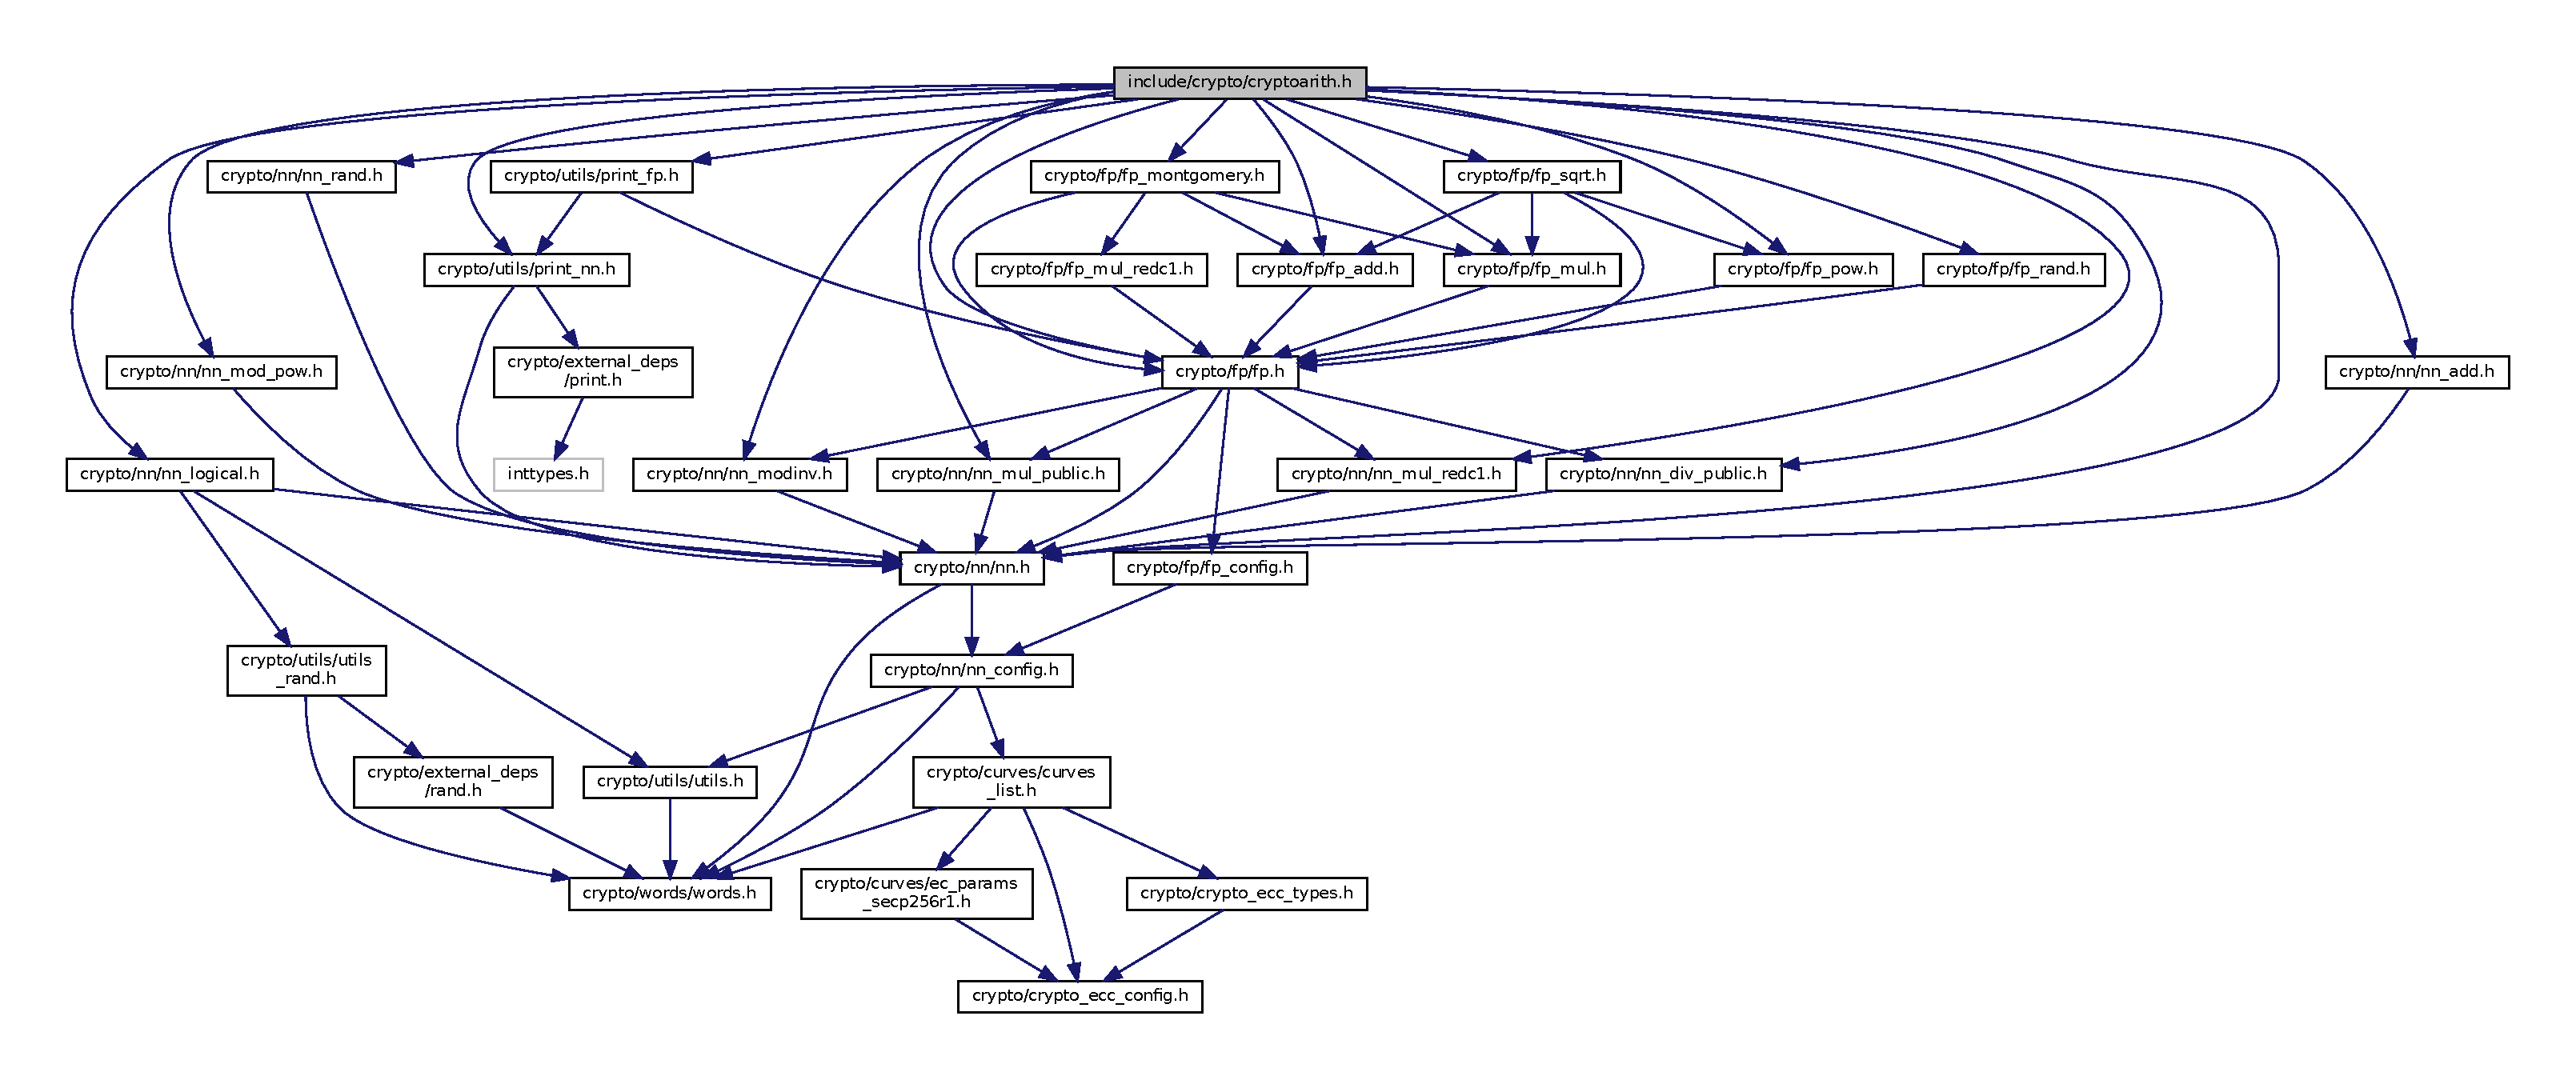
\includegraphics[scale=.4265, angle=-90]{dep-graph/cryptoarith.pdf}
\end{figure}
\newpage
\subsection{Modular Arithmetic}
\begin{figure}[h!]\centering
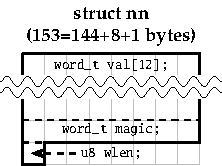
\includegraphics[scale=2.15]{struct-tikz/nn.pdf}
\end{figure}
\begin{lstlisting}[style=cstyle, caption={include/nn/nn.h}, captionpos=t]
#ifndef __NN_H__
#define __NN_H__

#include <crypto/words/words.h>
#include <crypto/nn/nn_config.h>

typedef struct {
	word_t val[BIT_LEN_WORDS(NN_MAX_BIT_LEN)];
	word_t magic;
	u8 wlen;
} nn;

typedef nn *nn_t;
typedef const nn *nn_src_t;

int nn_check_initialized(nn_src_t A);
int nn_is_initialized(nn_src_t A);
int nn_zero(nn_t A);
int nn_one(nn_t A);
int nn_set_word_value(nn_t A, word_t val);
void nn_uninit(nn_t A);
int nn_init(nn_t A, u16 len);
int nn_init_from_buf(nn_t A, const u8 *buf, u16 buflen);
int nn_cnd_swap(int cnd, nn_t in1, nn_t in2);
int nn_set_wlen(nn_t A, u8 new_wlen);
int nn_iszero(nn_src_t A, int *iszero);
int nn_isone(nn_src_t A, int *isone);
int nn_isodd(nn_src_t A, int *isodd);
int nn_cmp_word(nn_src_t in, word_t w, int *cmp);
int nn_cmp(nn_src_t A, nn_src_t B, int *cmp);
int nn_copy(nn_t dst_nn, nn_src_t src_nn);
int nn_normalize(nn_t in1);
int nn_export_to_buf(u8 *buf, u16 buflen, nn_src_t in_nn);
int nn_tabselect(nn_t out, u8 idx, nn_src_t *tab, u8 tabsize);

#endif /* __NN_H__ */
\end{lstlisting}

\newpage
\subsection{Finite Field}
\begin{figure}[h!]\centering
	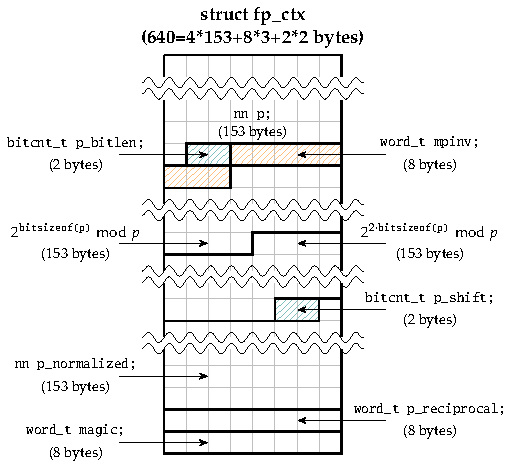
\includegraphics[scale=1.25]{struct-tikz/fp_ctx.pdf}
\end{figure}
\begin{lstlisting}[style=cstyle, caption={include/fp/fp.h}, captionpos=t]
#ifndef __FP_H__
#define __FP_H__

#include <crypto/nn/nn.h>
#include <crypto/nn/nn_div_public.h>
#include <crypto/nn/nn_modinv.h>
#include <crypto/nn/nn_mul_public.h>
#include <crypto/nn/nn_mul_redc1.h>
#include <crypto/fp/fp_config.h>

typedef struct {
	/*
	* Value of p (extended by one word to handle overflows in Fp). 
	* p_bitlen provides its length in bit.
	*/
	nn p;
	bitcnt_t p_bitlen;
	
	word_t mpinv;	/* -p^-1 mod 2^(bitsizeof(word_t)) */
	nn r;	/* 2^bitsizeof(p) mod p */
	nn r_square;	/* 2^(2*bitsizeof(p)) mod p */

	bitcnt_t p_shift;		/* clz(p) */
	nn p_normalized;	/* p << p_shift */
	word_t p_reciprocal;	/* floor(B^3/(DMSW(p_normalized) + 1)) - B */
	
	word_t magic;
} fp_ctx;

typedef fp_ctx *fp_ctx_t;
typedef const fp_ctx *fp_ctx_src_t;

int fp_ctx_check_initialized(fp_ctx_src_t ctx);
int fp_ctx_init(fp_ctx_t ctx, nn_src_t p, bitcnt_t p_bitlen, nn_src_t r, nn_src_t r_square, word_t mpinv, bitcnt_t p_shift, nn_src_t p_normalized, word_t p_reciprocal);
int fp_ctx_init_from_p(fp_ctx_t ctx, nn_src_t p);

/* Then the definition of our Fp elements */
typedef struct {
	nn fp_val;
	fp_ctx_src_t ctx;
	word_t magic;
} fp;

typedef fp *fp_t;
typedef const fp *fp_src_t;

int fp_check_initialized(fp_src_t in);
int fp_init(fp_t A, fp_ctx_src_t fpctx);
int fp_init_from_buf(fp_t A, fp_ctx_src_t fpctx, const u8 *buf, u16 buflen);
void fp_uninit(fp_t A);
int fp_set_nn(fp_t out, nn_src_t in);
int fp_zero(fp_t out);
int fp_one(fp_t out);
int fp_set_word_value(fp_t out, word_t val);
int fp_cmp(fp_src_t in1, fp_src_t in2, int *cmp);
int fp_iszero(fp_src_t in, int *iszero);
int fp_copy(fp_t out, fp_src_t in);
int fp_tabselect(fp_t out, u8 idx, fp_src_t *tab, u8 tabsize);
int fp_eq_or_opp(fp_src_t in1, fp_src_t in2, int *eq_or_opp);
int fp_import_from_buf(fp_t out_fp, const u8 *buf, u16 buflen);
int fp_export_to_buf(u8 *buf, u16 buflen, fp_src_t in_fp);

#endif /* __FP_H__ */
\end{lstlisting}

\begin{figure}[h!]\centering
	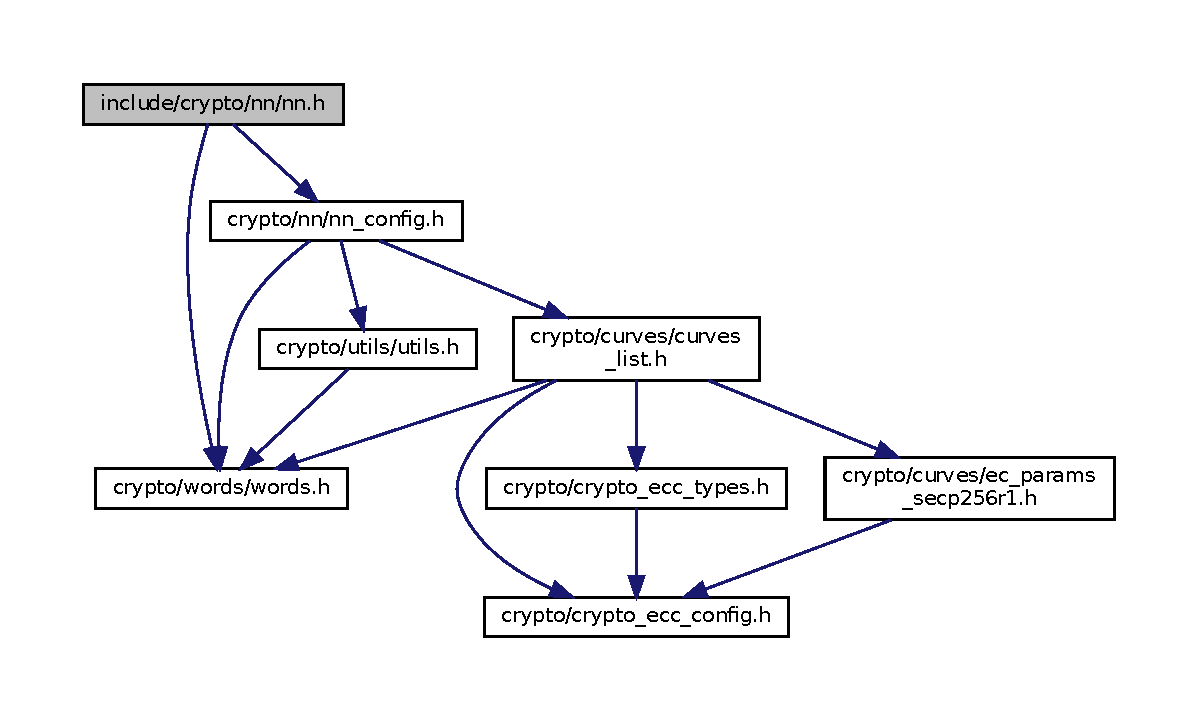
\includegraphics[scale=.7]{dep-graph/nn.pdf}
\end{figure}

\newpage
\section{Elliptic Curve Library}
\begin{figure}[h!]\centering
	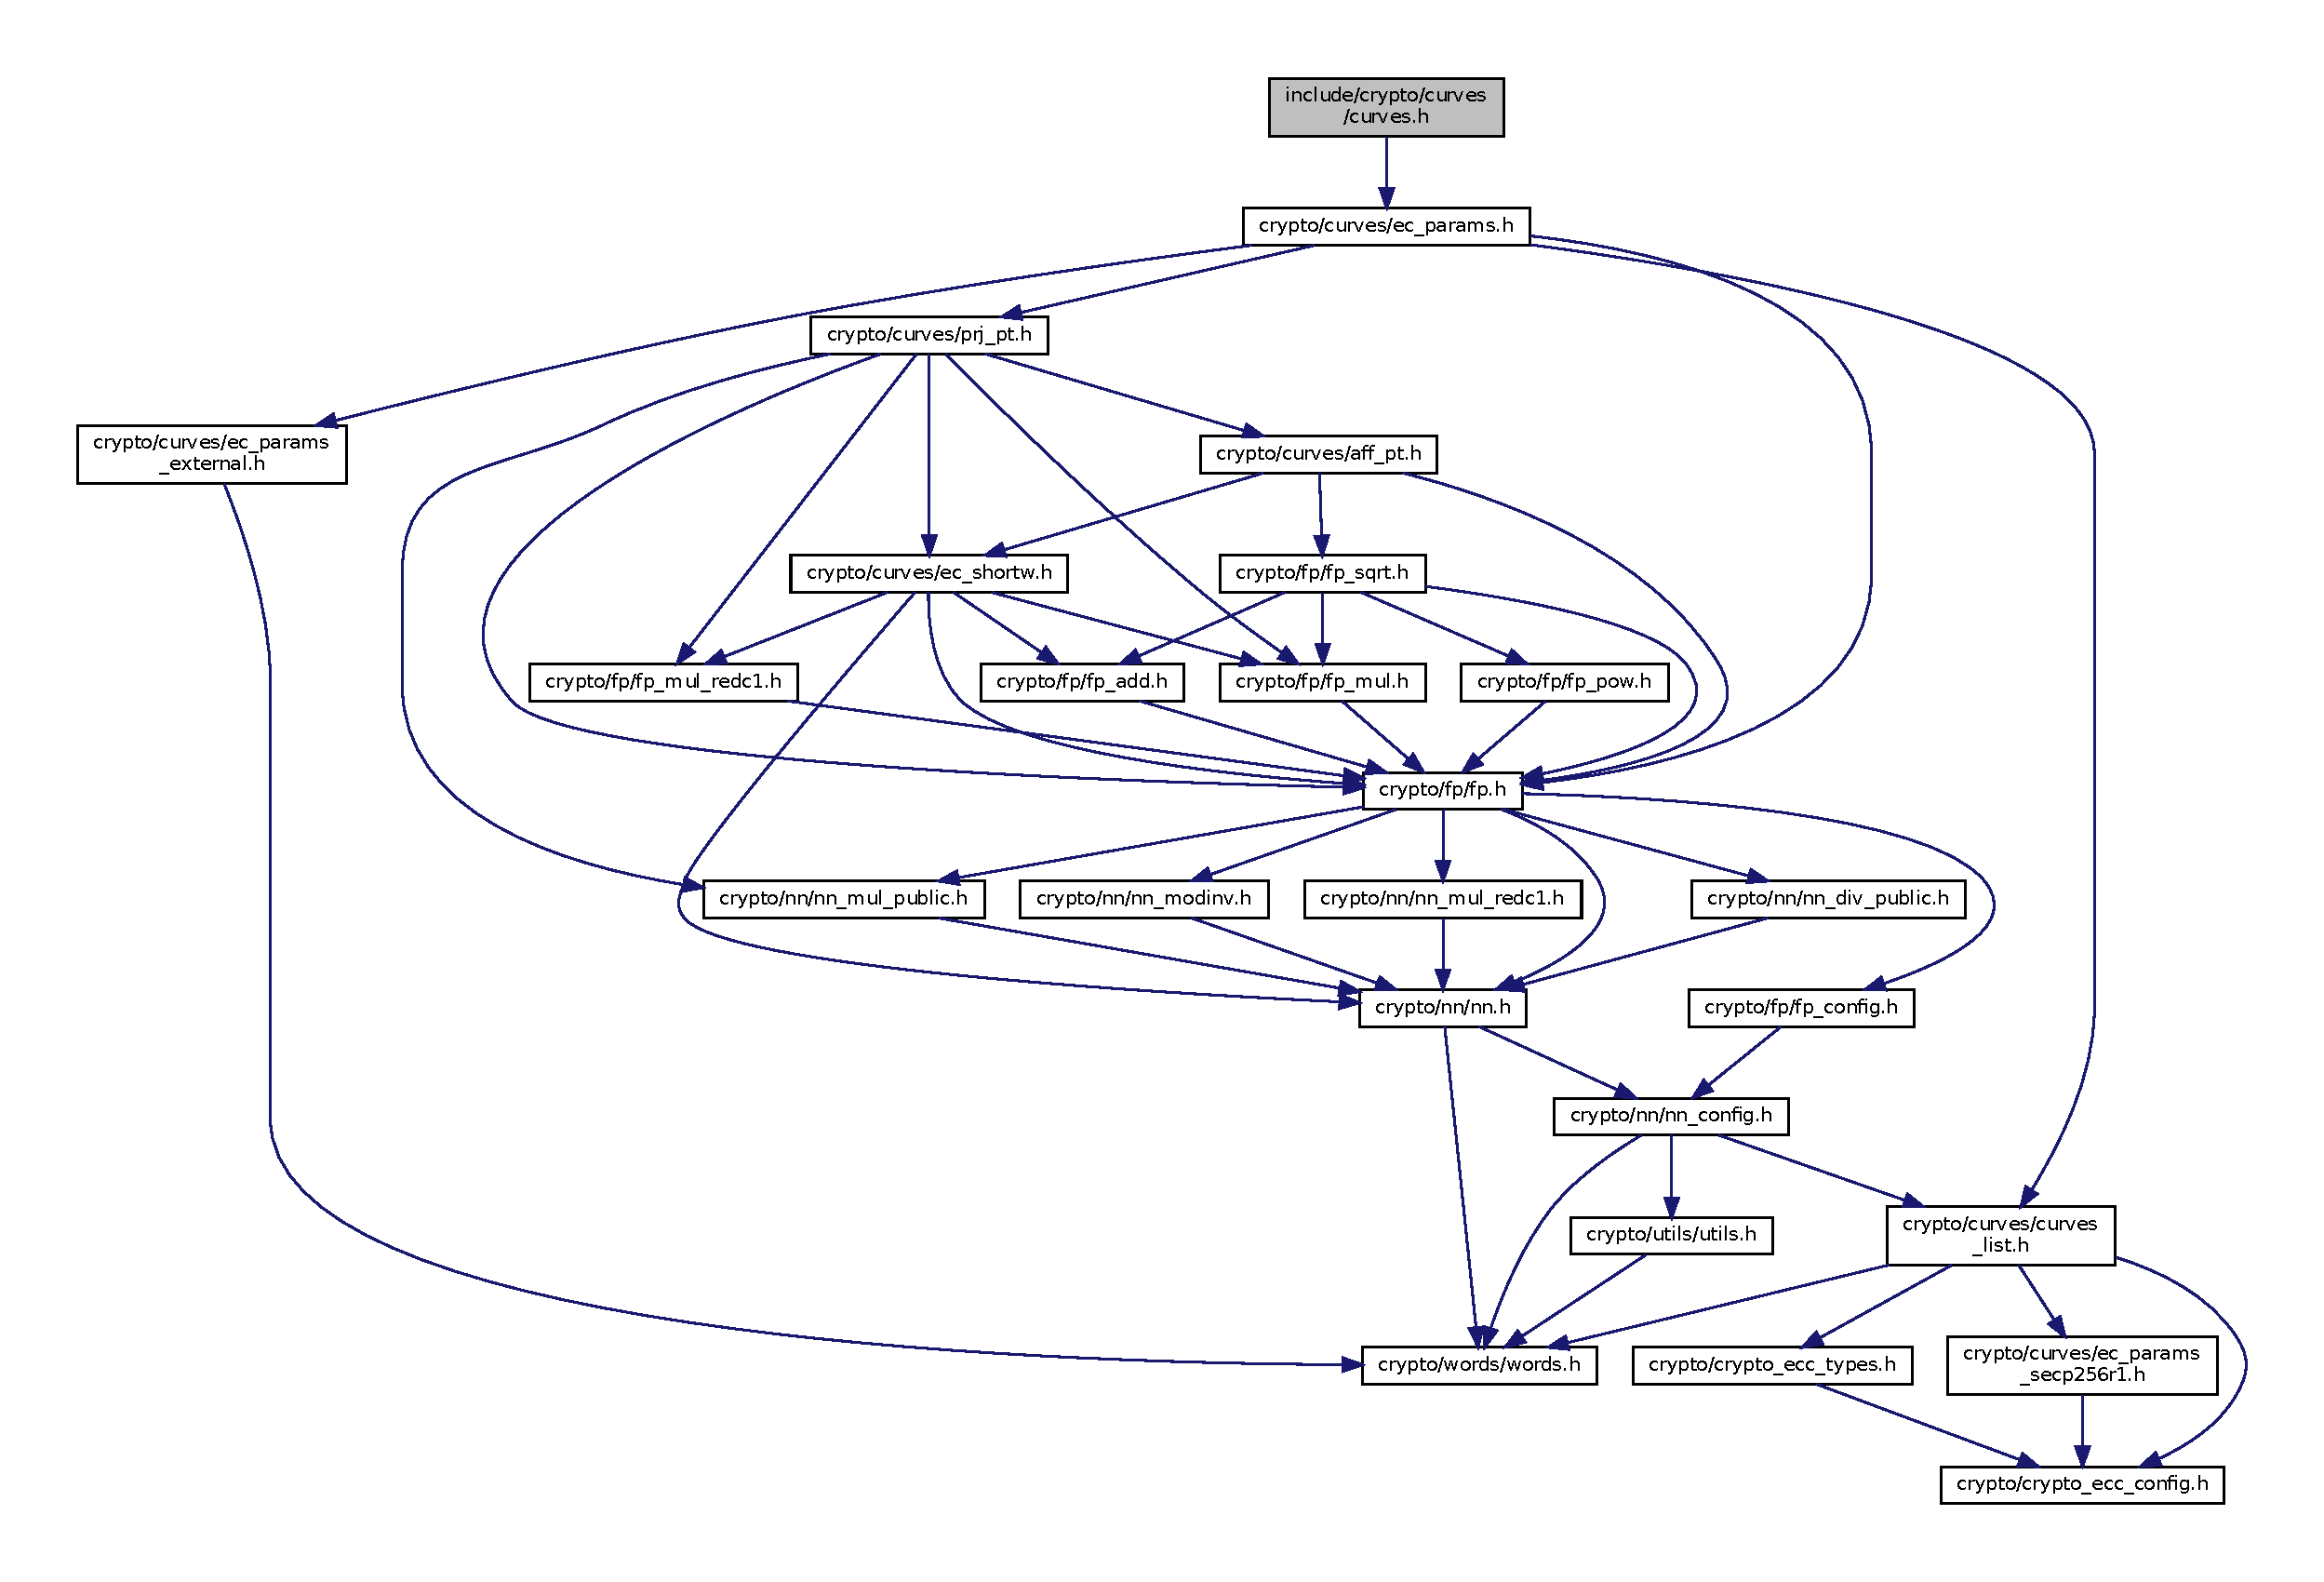
\includegraphics[scale=.545, angle=-90]{dep-graph/curves.pdf}
\end{figure}
\newpage
\subsection{Short Weierstrass Form}
\begin{lstlisting}[style=cstyle, caption={include/curves/ec\_shortw.h}, captionpos=t]
#ifndef __EC_SHORTW_H__
#define __EC_SHORTW_H__

#include <crypto/nn/nn.h>
#include <crypto/fp/fp.h>
#include <crypto/fp/fp_add.h>
#include <crypto/fp/fp_mul.h>
#include <crypto/fp/fp_mul_redc1.h>

typedef struct {
	fp a; fp b; fp a_monty;
#ifndef NO_USE_COMPLETE_FORMULAS
	fp b3; fp b_monty; fp b3_monty;
#endif
	nn order; /* curve order */
	word_t magic;
} ec_shortw_crv;

typedef ec_shortw_crv *ec_shortw_crv_t;
typedef const ec_shortw_crv *ec_shortw_crv_src_t;

int ec_shortw_crv_check_initialized(ec_shortw_crv_src_t crv);
int ec_shortw_crv_init(ec_shortw_crv_t crv, fp_src_t a, fp_src_t b, nn_src_t order);
void ec_shortw_crv_uninit(ec_shortw_crv_t crv);

#endif /* __EC_SHORTW_H__ */
\end{lstlisting}
\begin{figure}[h!]\centering
	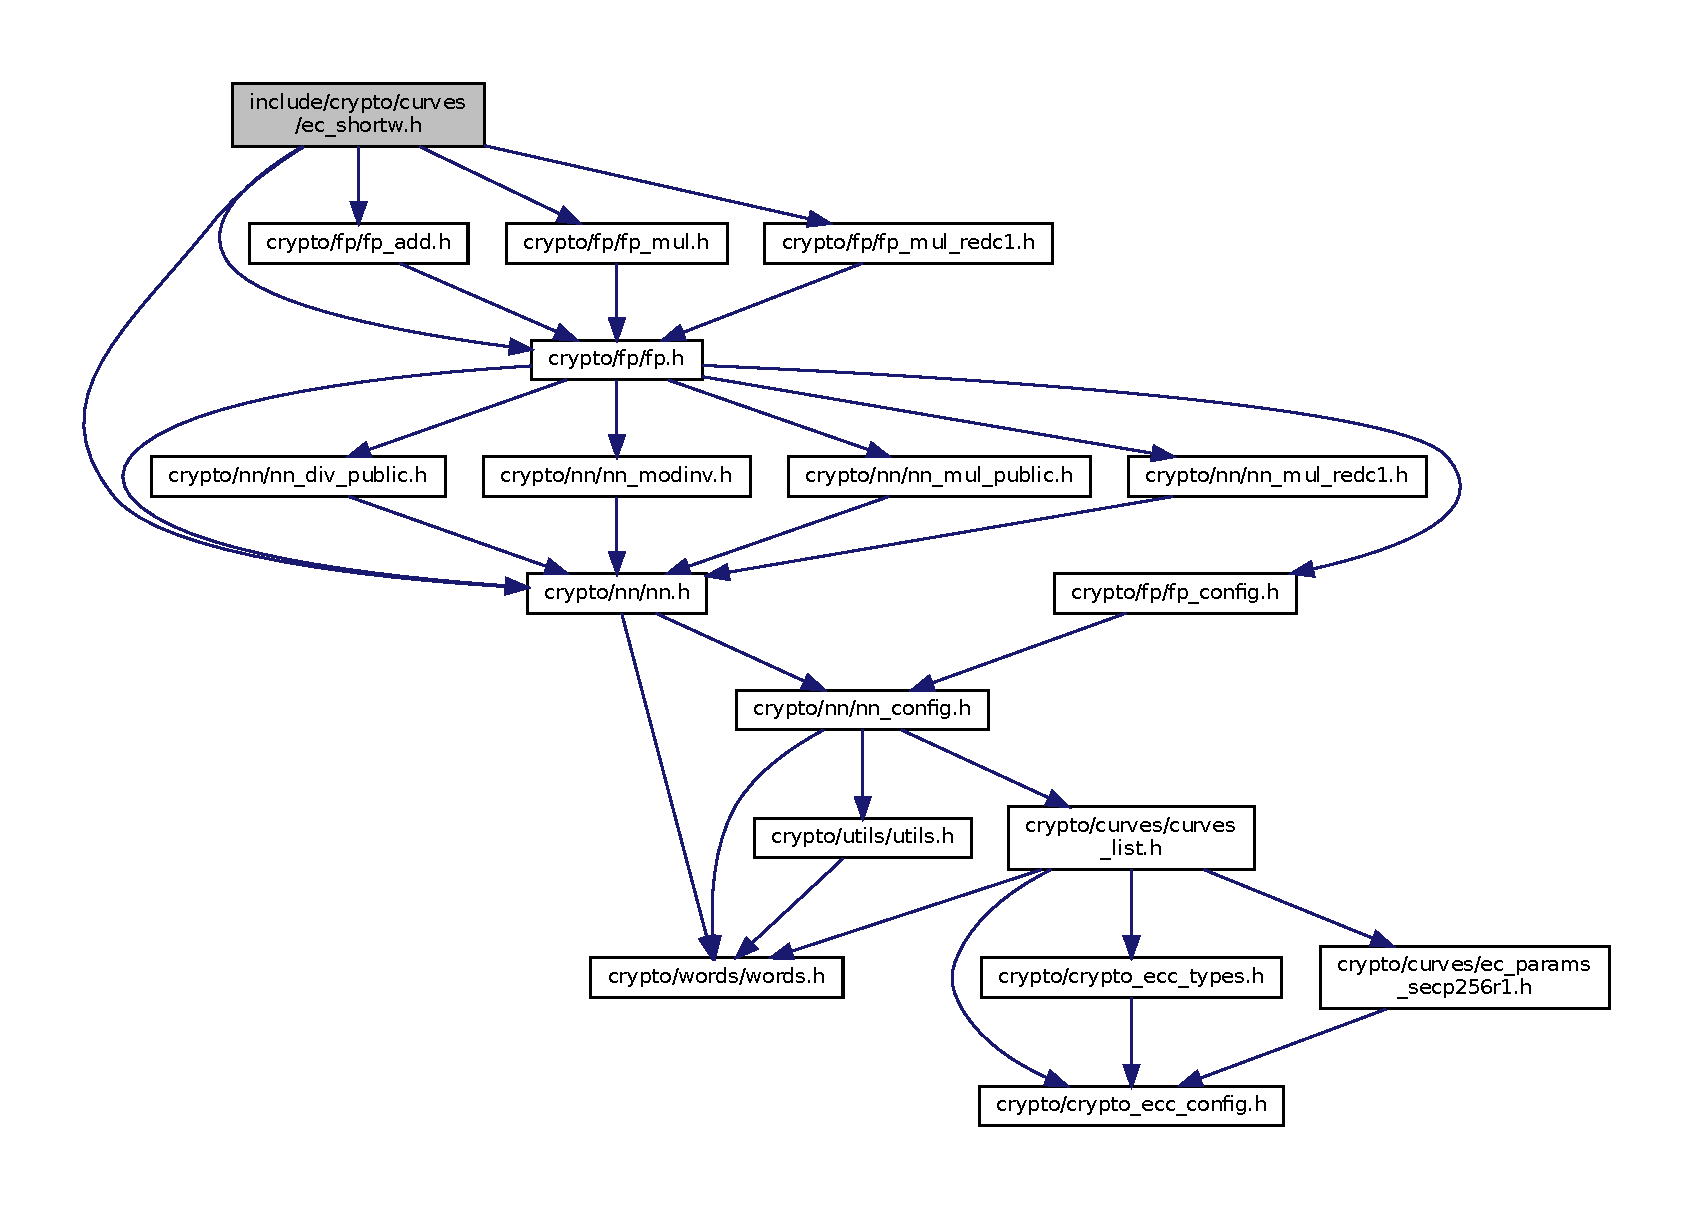
\includegraphics[scale=.545]{dep-graph/ec_shortw.pdf}
\end{figure}

\newpage
\subsection{Points of Affine Coordinate}
\begin{lstlisting}[style=cstyle, caption={include/curves/aff\_pt.h}, captionpos=t]
#ifndef __AFF_PT_H__
#define __AFF_PT_H__
#include <crypto/fp/fp.h>
#include <crypto/fp/fp_sqrt.h>
#include <crypto/curves/ec_shortw.h>
typedef struct {
	fp x; fp y; 
	ec_shortw_crv_src_t crv;
	word_t magic;
} aff_pt;
typedef aff_pt *aff_pt_t;
typedef const aff_pt_t aff_pt_src_t;
int aff_pt_check_initialized(aff_pt_src_t in);
int aff_pt_init(aff_pt_t in, ec_shortw_crv_src_t curve);
int aff_pt_init_from_coords(aff_pt_t in, ec_shortw_crv_src_t curve, fp_src_t xcoord, fp_src_t ycoord);
void aff_pt_uninit(aff_pt_t in);
int aff_pt_y_from_x(fp_t y1, fp_t y2, fp_src_t x, ec_shortw_crv_src_t curve);
int is_on_shortw_curve(fp_src_t x, fp_src_t y, ec_shortw_crv_src_t curve, int *on_curve);
int aff_pt_is_on_curve(aff_pt_src_t pt, int *on_curve);
int ec_shortw_aff_copy(aff_pt_t out, aff_pt_src_t in);
int ec_shortw_aff_cmp(aff_pt_src_t in1, aff_pt_src_t in2, int *cmp);
int ec_shortw_aff_eq_or_opp(aff_pt_src_t in1, aff_pt_src_t in2, int *eq_or_opp);
int aff_pt_import_from_buf(aff_pt_t pt, const u8 *pt_buf, u16 pt_buf_len, ec_shortw_crv_src_t crv);
int aff_pt_export_to_buf(aff_pt_src_t pt, u8 *pt_buf, u32 pt_buf_len);
#endif /* __AFF_PT_H__ */

\end{lstlisting}
\begin{figure}[h!]\centering
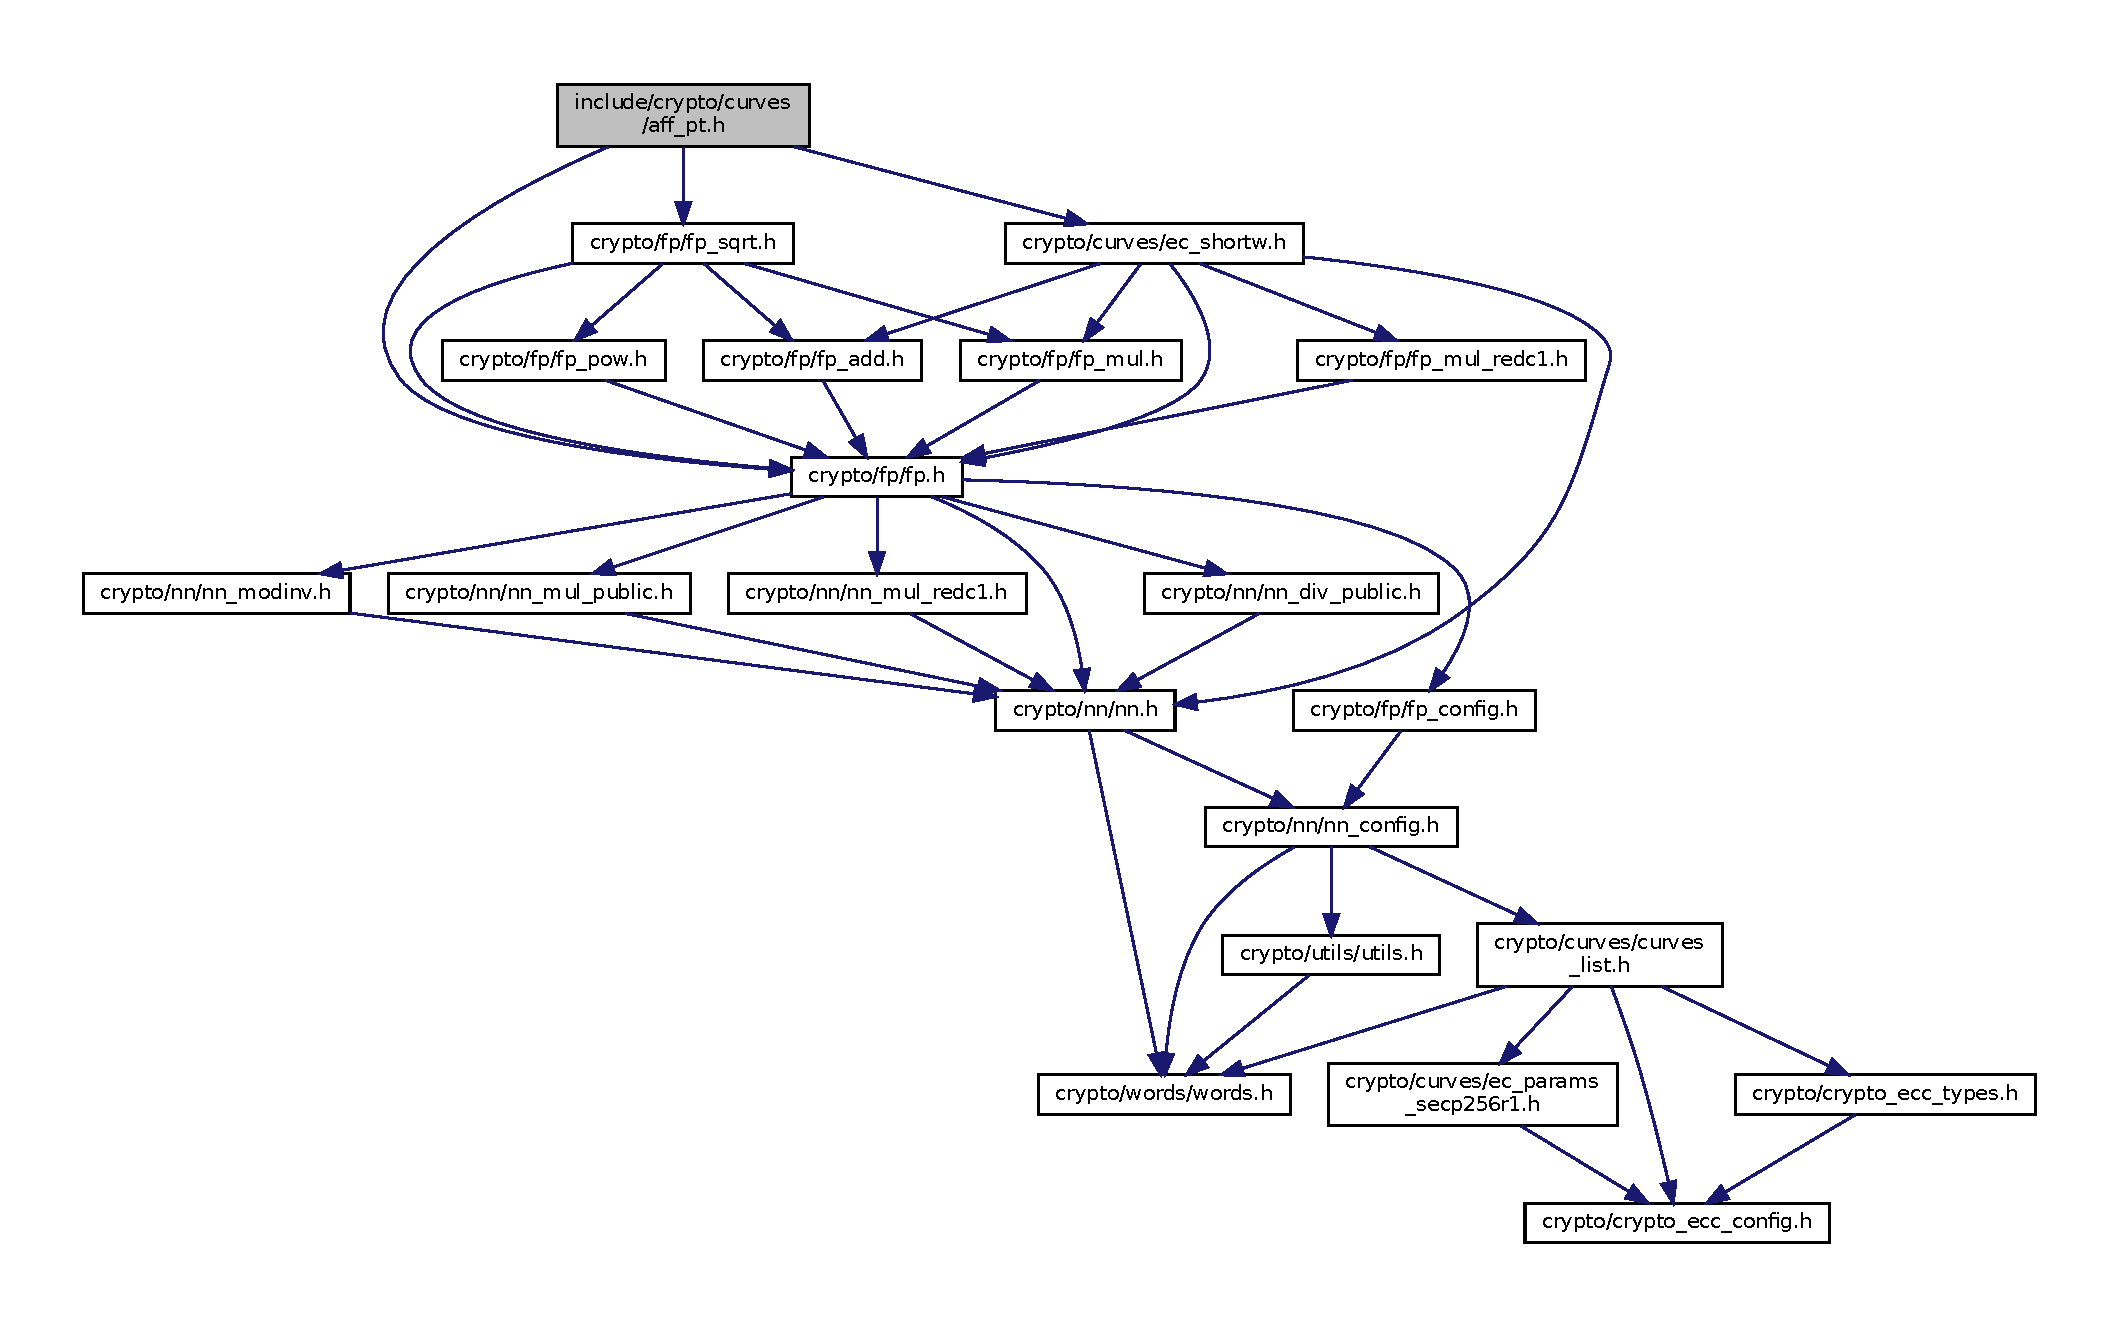
\includegraphics[scale=.45]{dep-graph/aff_pt.pdf}
\end{figure}
\newpage

\subsection{Points of Projective Coordinate}
\begin{lstlisting}[style=cstyle, caption={include/curves/prj\_pt.h}, captionpos=t]
#ifndef __PRJ_PT_H__
#define __PRJ_PT_H__

#include <crypto/nn/nn_mul_public.h>
#include <crypto/fp/fp.h>
#include <crypto/fp/fp_mul.h>
#include <crypto/fp/fp_mul_redc1.h>
#include <crypto/curves/ec_shortw.h>
#include <crypto/curves/aff_pt.h>

typedef struct {
	fp X; fp Y; fp Z;
	ec_shortw_crv_src_t crv;
	word_t magic;
} prj_pt;

typedef prj_pt *prj_pt_t;
typedef const prj_pt *prj_pt_src_t;
typedef enum {
	PUBLIC_PT = 0,
	PRIVATE_PT = 1
} prj_pt_sensitivity;

int prj_pt_check_initialized(prj_pt_src_t in);
int prj_pt_init(prj_pt_t in, ec_shortw_crv_src_t curve);
int prj_pt_init_from_coords(prj_pt_t in, ec_shortw_crv_src_t curve, fp_src_t xcoord, fp_src_t ycoord, fp_src_t zcoord);
void prj_pt_uninit(prj_pt_t in);
int prj_pt_zero(prj_pt_t out);
int prj_pt_iszero(prj_pt_src_t in, int *iszero);
int prj_pt_is_on_curve(prj_pt_src_t in, int *on_curve);
int prj_pt_copy(prj_pt_t out, prj_pt_src_t in);
int prj_pt_to_aff(aff_pt_t out, prj_pt_src_t in);
int prj_pt_unique(prj_pt_t out, prj_pt_src_t in);
int ec_shortw_aff_to_prj(prj_pt_t out, aff_pt_src_t in);
int prj_pt_cmp(prj_pt_src_t in1, prj_pt_src_t in2, int *cmp);
int prj_pt_eq_or_opp(prj_pt_src_t in1, prj_pt_src_t in2, int *eq_or_opp);
int prj_pt_neg(prj_pt_t out, prj_pt_src_t in);
int prj_pt_add(prj_pt_t sum, prj_pt_src_t in1, prj_pt_src_t in2);
int prj_pt_dbl(prj_pt_t dbl, prj_pt_src_t in);
int prj_pt_mul(prj_pt_t out, nn_src_t m, prj_pt_src_t in);
int prj_pt_mul_blind(prj_pt_t out, nn_src_t m, prj_pt_src_t in);
/* XXX: WARNING: this function must only be used on public points! */
int _prj_pt_unprotected_mult(prj_pt_t out, nn_src_t cofactor, prj_pt_src_t public_in);
int check_prj_pt_order(prj_pt_src_t in_shortw, nn_src_t in_isorder, prj_pt_sensitivity s, int *check);
int prj_pt_import_from_buf(prj_pt_t pt, const u8 *pt_buf, u16 pt_buf_len, ec_shortw_crv_src_t crv);
int prj_pt_import_from_aff_buf(prj_pt_t pt, const u8 *pt_buf, u16 pt_buf_len, ec_shortw_crv_src_t crv);
int prj_pt_export_to_buf(prj_pt_src_t pt, u8 *pt_buf, u32 pt_buf_len);
int prj_pt_export_to_aff_buf(prj_pt_src_t pt, u8 *pt_buf, u32 pt_buf_len);

#endif /* __PRJ_PT_H__ */
\end{lstlisting}
\begin{figure}[h!]\centering
	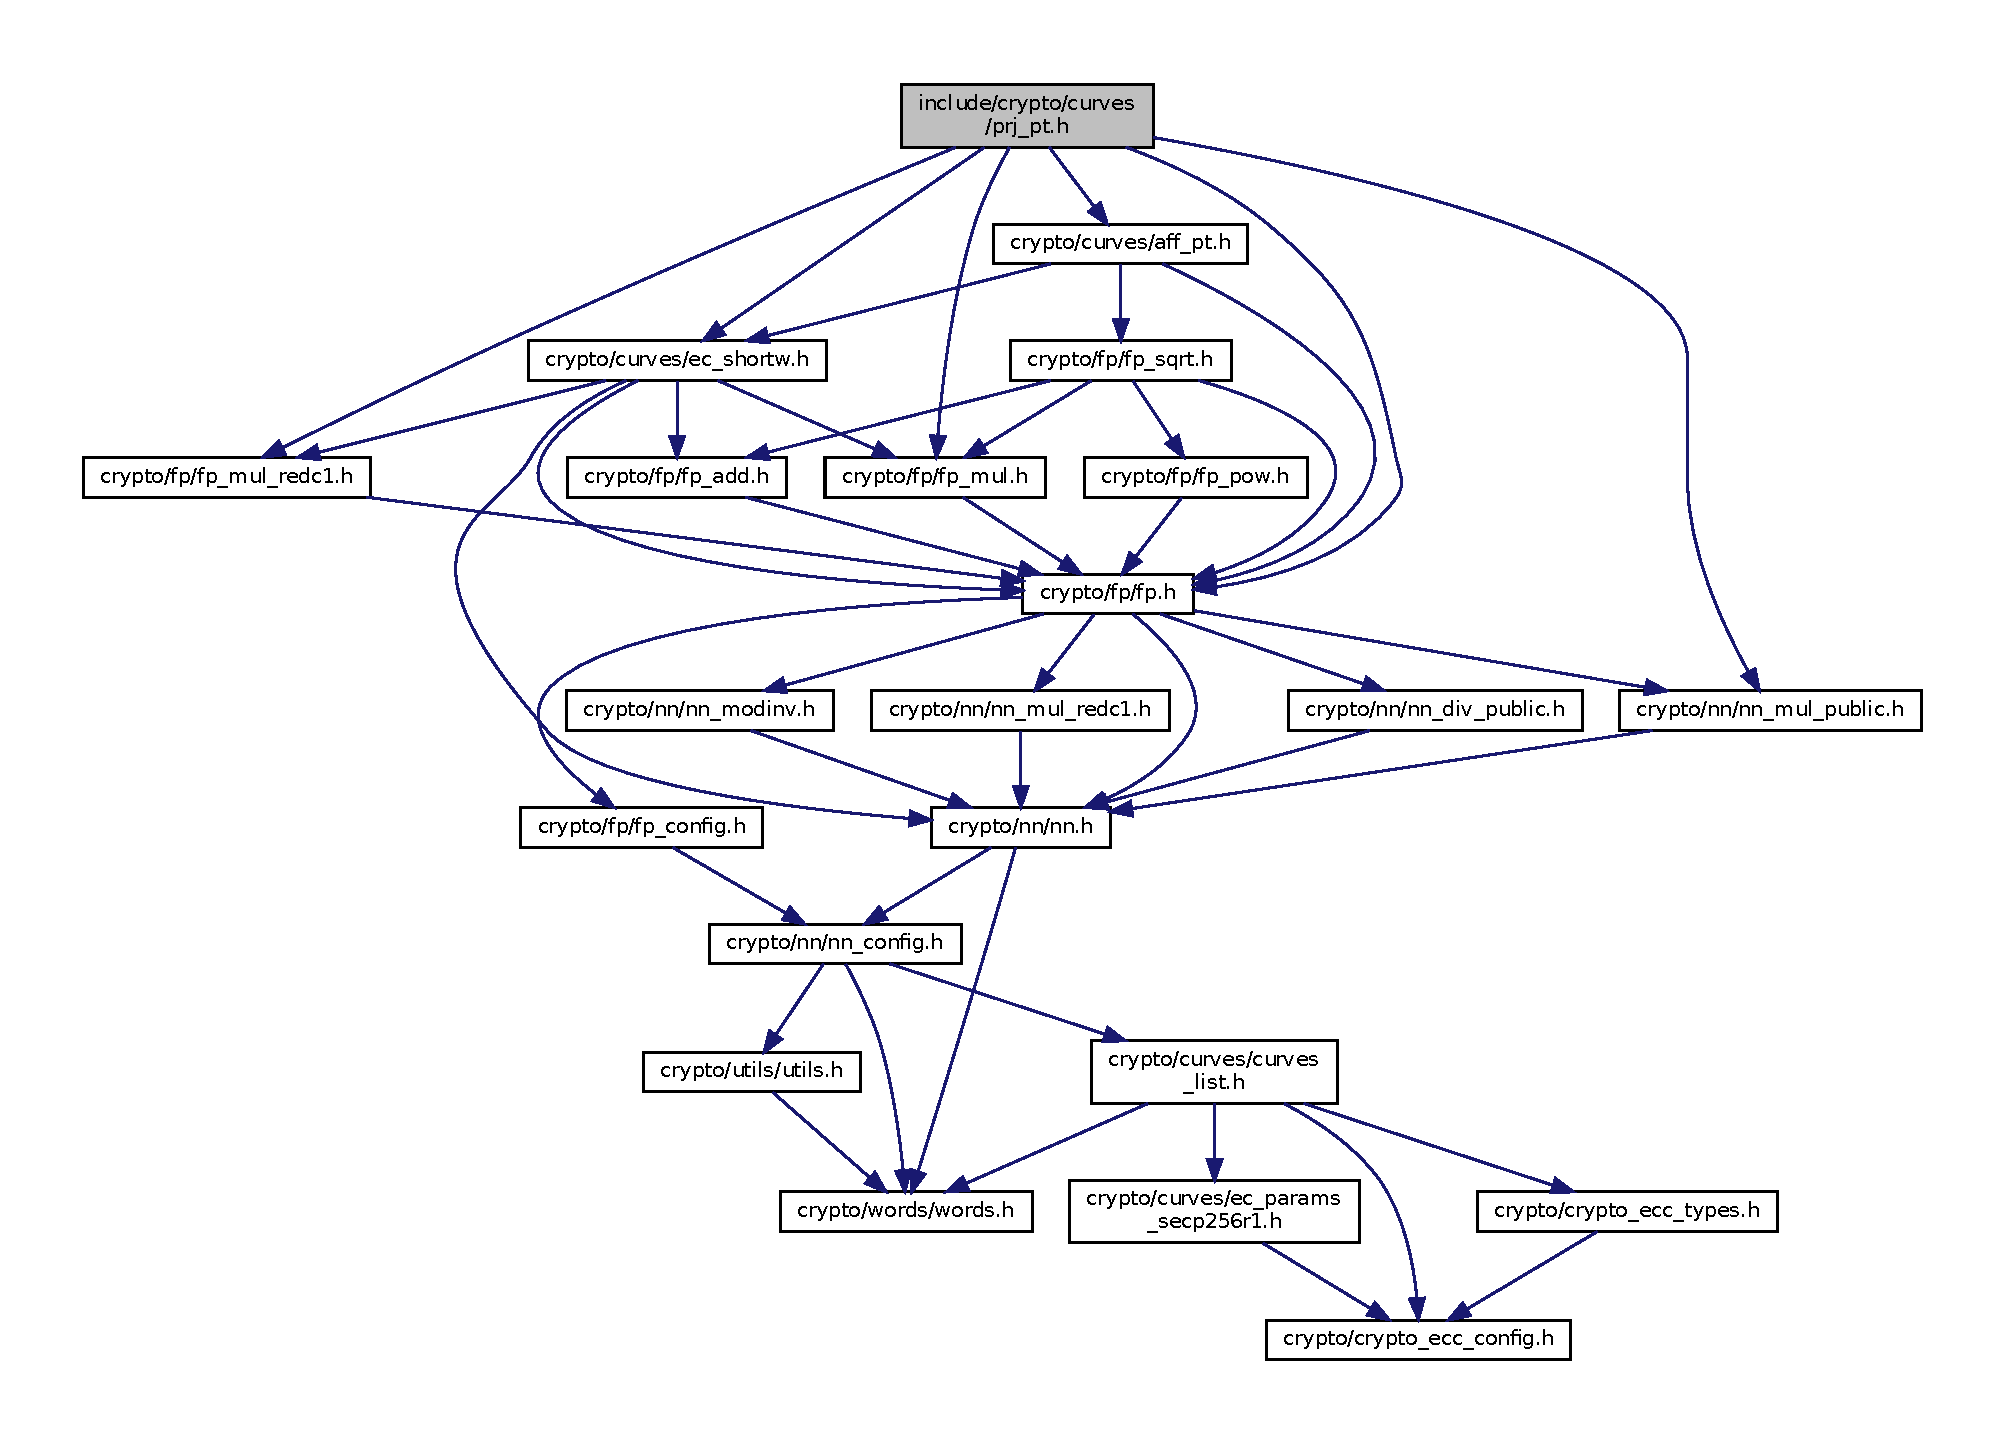
\includegraphics[scale=.675, angle=-90]{dep-graph/prj_pt.pdf}
\end{figure}

\newpage
\ \\
\section{Elliptic Curve Digital Signature Algorithm Library}
\begin{lstlisting}[style=cstyle, caption={include/curves/prj\_pt.h}, captionpos=t]
#include <crypto/crypto_ecc_config.h>
#include <crypto/crypto_ecc_types.h>
#ifndef __ECDSA_COMMON_H__
#define __ECDSA_COMMON_H__

#include <crypto/words/words.h>
#include <crypto/sig/ec_key.h>
#include <crypto/hash/hash_algs.h>
#include <crypto/curves/curves.h>
#include <crypto/utils/utils.h>

#define ECDSA_R_LEN(q_bit_len)  (BYTECEIL(q_bit_len))
#define ECDSA_S_LEN(q_bit_len)  (BYTECEIL(q_bit_len))
#define ECDSA_SIGLEN(q_bit_len) (ECDSA_R_LEN(q_bit_len) + \
ECDSA_S_LEN(q_bit_len))
#define ECDSA_MAX_SIGLEN ECDSA_SIGLEN(CURVES_MAX_Q_BIT_LEN)

/*
* Compute max signature length for all the mechanisms enabled in the library (see lib_ecc_config.h). 
* Having that done during
* preprocessing sadly requires some verbosity.
*/
#ifndef EC_MAX_SIGLEN
#define EC_MAX_SIGLEN 0
#endif
#if ((EC_MAX_SIGLEN) < (ECDSA_MAX_SIGLEN))
#undef EC_MAX_SIGLEN
#define EC_MAX_SIGLEN ECDSA_MAX_SIGLEN
#endif

typedef struct {
	hash_context h_ctx;
	word_t magic;
} ecdsa_sign_data;

struct ec_sign_context;

int __ecdsa_init_pub_key(ec_pub_key *out_pub, const ec_priv_key *in_priv, ec_alg_type key_type);

int __ecdsa_siglen(u16 p_bit_len, u16 q_bit_len, u8 hsize, u8 blocksize, u8 *siglen);
int __ecdsa_sign_init(struct ec_sign_context *ctx, ec_alg_type key_type);
int __ecdsa_sign_update(struct ec_sign_context *ctx,
const u8 *chunk, u32 chunklen, ec_alg_type key_type);
int __ecdsa_sign_finalize(struct ec_sign_context *ctx, u8 *sig, u8 siglen, ec_alg_type key_type);

typedef struct {
	nn r; nn s;
	hash_context h_ctx;
	word_t magic;
} ecdsa_verify_data;

struct ec_verify_context;

int __ecdsa_verify_init(struct ec_verify_context *ctx,
const u8 *sig, u8 siglen, ec_alg_type key_type);
int __ecdsa_verify_update(struct ec_verify_context *ctx,
const u8 *chunk, u32 chunklen, ec_alg_type key_type);
int __ecdsa_verify_finalize(struct ec_verify_context *ctx, ec_alg_type key_type);

int __ecdsa_public_key_from_sig(ec_pub_key *out_pub1, ec_pub_key *out_pub2, const ec_params *params, const u8 *sig, u8 siglen, const u8 *hash, u8 hsize, ec_alg_type key_type);

#endif /* __ECDSA_COMMON_H__ */
\end{lstlisting}
\begin{figure}[h!]\centering
	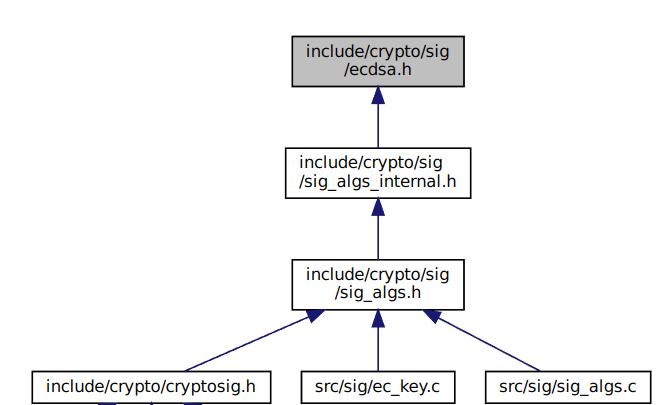
\includegraphics[scale=.7]{dep-graph/ecdsa.png}
\end{figure}

\newpage
\section{Build with Makefile}
This section describes the build system for generating (static) libraries, driven by a single GNU Makefile. It covers compiler settings, directory layout, source discovery, and all available targets.


\paragraph{Build without Makefile}\ \\
\begin{lstlisting}[numbers=none]
mkdir -p obj/nn obj/fp obj/utils
gcc -MMD -MP -c -O2 -std=c99 -Wall -Wextra -Iinclude -fPIC -o obj/nn/nn_add.o src/nn/nn_add.c
gcc -MMD -MP -c -O2 -std=c99 -Wall -Wextra -Iinclude -fPIC -o obj/nn/nn.o src/nn/nn.c
gcc -MMD -MP -c -O2 -std=c99 -Wall -Wextra -Iinclude -fPIC -o obj/nn/nn_div.o src/nn/nn_div.c
gcc -MMD -MP -c -O2 -std=c99 -Wall -Wextra -Iinclude -fPIC -o obj/nn/nn_logical.o src/nn/nn_logical.c
gcc -MMD -MP -c -O2 -std=c99 -Wall -Wextra -Iinclude -fPIC -o obj/nn/nn_modinv.o src/nn/nn_modinv.c
gcc -MMD -MP -c -O2 -std=c99 -Wall -Wextra -Iinclude -fPIC -o obj/nn/nn_mod_pow.o src/nn/nn_mod_pow.c
gcc -MMD -MP -c -O2 -std=c99 -Wall -Wextra -Iinclude -fPIC -o obj/nn/nn_mul.o src/nn/nn_mul.c
gcc -MMD -MP -c -O2 -std=c99 -Wall -Wextra -Iinclude -fPIC -o obj/nn/nn_mul_redc1.o src/nn/nn_mul_redc1.c
gcc -MMD -MP -c -O2 -std=c99 -Wall -Wextra -Iinclude -fPIC -o obj/nn/nn_rand.o src/nn/nn_rand.c

gcc -MMD -MP -c -O2 -std=c99 -Wall -Wextra -Iinclude -fPIC -o obj/fp/fp_add.o src/fp/fp_add.c
gcc -MMD -MP -c -O2 -std=c99 -Wall -Wextra -Iinclude -fPIC -o obj/fp/fp.o src/fp/fp.c
gcc -MMD -MP -c -O2 -std=c99 -Wall -Wextra -Iinclude -fPIC -o obj/fp/fp_mul.o src/fp/fp_mul.c
gcc -MMD -MP -c -O2 -std=c99 -Wall -Wextra -Iinclude -fPIC -o obj/fp/fp_mul_redc1.o src/fp/fp_mul_redc1.c
gcc -MMD -MP -c -O2 -std=c99 -Wall -Wextra -Iinclude -fPIC -o obj/fp/fp_pow.o src/fp/fp_pow.c
gcc -MMD -MP -c -O2 -std=c99 -Wall -Wextra -Iinclude -fPIC -o obj/fp/fp_rand.o src/fp/fp_rand.c
gcc -MMD -MP -c -O2 -std=c99 -Wall -Wextra -Iinclude -fPIC -o obj/fp/fp_sqrt.o src/fp/fp_sqrt.c

gcc -MMD -MP -c -O2 -std=c99 -Wall -Wextra -Iinclude -fPIC -o obj/utils/utils.o src/utils/utils.c
gcc -MMD -MP -c -O2 -std=c99 -Wall -Wextra -Iinclude -fPIC -o obj/utils/utils_rand.o src/utils/utils_rand.c
gcc -MMD -MP -c -O2 -std=c99 -Wall -Wextra -Iinclude -fPIC -o obj/utils/print_nn.o src/utils/print_nn.c
gcc -MMD -MP -c -O2 -std=c99 -Wall -Wextra -Iinclude -fPIC -o obj/utils/print_fp.o src/utils/print_fp.c
gcc -MMD -MP -c -O2 -std=c99 -Wall -Wextra -Iinclude -fPIC -o obj/utils/print_buf.o src/utils/print_buf.c

mkdir -p obj/external_deps
gcc -MMD -MP -c -O2 -std=c99 -Wall -Wextra -Iinclude -fPIC -o obj/external_deps/print.o src/external_deps/print.c
gcc -MMD -MP -c -O2 -std=c99 -Wall -Wextra -Iinclude -fPIC -o obj/external_deps/rand.o src/external_deps/rand.c
gcc -MMD -MP -c -O2 -std=c99 -Wall -Wextra -Iinclude -fPIC -o obj/external_deps/time.o src/external_deps/time.c

mkdir -p lib
ar rcs lib/libarith.a \
	obj/fp/fp_add.o obj/fp/fp.o obj/fp/fp_mul.o obj/fp/fp_mul_redc1.o obj/fp/fp_pow.o obj/fp/fp_rand.o obj/fp/fp_sqrt.o \
	obj/nn/nn_add.o obj/nn/nn.o obj/nn/nn_div.o obj/nn/nn_logical.o obj/nn/nn_modinv.o obj/nn/nn_mod_pow.o obj/nn/nn_mul.o obj/nn/nn_mul_redc1.o obj/nn/nn_rand.o \
	obj/utils/utils.o obj/utils/utils_rand.o obj/utils/print_nn.o obj/utils/print_fp.o obj/utils/print_buf.o \
	obj/external_deps/print.o obj/external_deps/rand.o obj/external_deps/time.o 

mkdir -p obj/curves
gcc -MMD -MP -c -O2 -std=c99 -Wall -Wextra -Iinclude -fPIC -o obj/curves/aff_pt.o src/curves/aff_pt.c
gcc -MMD -MP -c -O2 -std=c99 -Wall -Wextra -Iinclude -fPIC -o obj/curves/curves.o src/curves/curves.c
gcc -MMD -MP -c -O2 -std=c99 -Wall -Wextra -Iinclude -fPIC -o obj/curves/ec_params.o src/curves/ec_params.c
gcc -MMD -MP -c -O2 -std=c99 -Wall -Wextra -Iinclude -fPIC -o obj/curves/ec_shortw.o src/curves/ec_shortw.c
gcc -MMD -MP -c -O2 -std=c99 -Wall -Wextra -Iinclude -fPIC -o obj/curves/prj_pt.o src/curves/prj_pt.c
gcc -MMD -MP -c -O2 -std=c99 -Wall -Wextra -Iinclude -fPIC -o obj/utils/print_curves.o src/utils/print_curves.c

ar rcs lib/libec.a \
	obj/fp/fp_add.o obj/fp/fp.o obj/fp/fp_mul.o obj/fp/fp_mul_redc1.o obj/fp/fp_pow.o obj/fp/fp_rand.o obj/fp/fp_sqrt.o \
	obj/nn/nn_add.o obj/nn/nn.o obj/nn/nn_div.o obj/nn/nn_logical.o obj/nn/nn_modinv.o obj/nn/nn_mod_pow.o obj/nn/nn_mul.o obj/nn/nn_mul_redc1.o obj/nn/nn_rand.o \
	obj/utils/utils.o obj/utils/utils_rand.o obj/utils/print_nn.o obj/utils/print_fp.o obj/utils/print_buf.o \
	obj/curves/aff_pt.o obj/curves/curves.o obj/curves/ec_params.o obj/curves/ec_shortw.o obj/curves/prj_pt.o \
	obj/utils/print_curves.o \
	obj/external_deps/print.o obj/external_deps/rand.o obj/external_deps/time.o 

mkdir -p obj/hash obj/sig
gcc -MMD -MP -c -O2 -std=c99 -Wall -Wextra -Iinclude -fPIC -o obj/hash/sha256.o src/hash/sha256.c
gcc -MMD -MP -c -O2 -std=c99 -Wall -Wextra -Iinclude -fPIC -o obj/hash/sha3-256.o src/hash/sha3-256.c
gcc -MMD -MP -c -O2 -std=c99 -Wall -Wextra -Iinclude -fPIC -o obj/hash/sha3.o src/hash/sha3.c
gcc -MMD -MP -c -O2 -std=c99 -Wall -Wextra -Iinclude -fPIC -o obj/hash/shake256.o src/hash/shake256.c
gcc -MMD -MP -c -O2 -std=c99 -Wall -Wextra -Iinclude -fPIC -o obj/hash/shake.o src/hash/shake.c
gcc -MMD -MP -c -O2 -std=c99 -Wall -Wextra -Iinclude -fPIC -o obj/hash/hash_algs.o src/hash/hash_algs.c
gcc -MMD -MP -c -O2 -std=c99 -Wall -Wextra -Iinclude -fPIC -o obj/hash/hmac.o src/hash/hmac.c

gcc -MMD -MP -c -O2 -std=c99 -Wall -Wextra -Iinclude -fPIC -o obj/sig/ecdsa.o src/sig/ecdsa.c
gcc -MMD -MP -c -O2 -std=c99 -Wall -Wextra -Iinclude -fPIC -o obj/sig/ecdsa_common.o src/sig/ecdsa_common.c
gcc -MMD -MP -c -O2 -std=c99 -Wall -Wextra -Iinclude -fPIC -o obj/sig/sig_algs.o src/sig/sig_algs.c
gcc -MMD -MP -c -O2 -std=c99 -Wall -Wextra -Iinclude -fPIC -o obj/sig/ec_key.o src/sig/ec_key.c
gcc -MMD -MP -c -O2 -std=c99 -Wall -Wextra -Iinclude -fPIC -o obj/utils/print_keys.o src/utils/print_keys.c

ar rcs lib/libsign.a \
	obj/fp/fp_add.o obj/fp/fp.o obj/fp/fp_mul.o obj/fp/fp_mul_redc1.o obj/fp/fp_pow.o obj/fp/fp_rand.o obj/fp/fp_sqrt.o \
	obj/nn/nn_add.o obj/nn/nn.o obj/nn/nn_div.o obj/nn/nn_logical.o obj/nn/nn_modinv.o obj/nn/nn_mod_pow.o obj/nn/nn_mul.o obj/nn/nn_mul_redc1.o obj/nn/nn_rand.o \
	obj/utils/utils.o obj/utils/utils_rand.o obj/utils/print_nn.o obj/utils/print_fp.o obj/utils/print_buf.o \
	obj/curves/aff_pt.o obj/curves/curves.o obj/curves/ec_params.o obj/curves/ec_shortw.o obj/curves/prj_pt.o \
	obj/utils/print_curves.o \
	obj/hash/sha256.o obj/hash/sha3-256.o obj/hash/sha3.o obj/hash/shake256.o obj/hash/shake.o obj/hash/hash_algs.o obj/hash/hmac.o \
	obj/sig/ecdsa.o obj/sig/ecdsa_common.o obj/sig/sig_algs.o obj/sig/ec_key.o \
	obj/utils/print_keys.o \
	obj/external_deps/print.o obj/external_deps/rand.o obj/external_deps/time.o 
\end{lstlisting}

\newpage
\paragraph{Build with Makefile}\ \\
\ \\
\textbf{[gcc (GNU Compiler Collection)]}
\begin{itemize}
	\item \texttt{gcc}: compiles and links source code.
\end{itemize}
\textbf{[ar \texttt{rcs} (GNU Archiver)]}
\begin{itemize}
	\item \texttt{ar rcs}: creates or updates static library archives.
	\begin{itemize}
		\item \texttt{r}: ``replace'' -- add or replace files in the archive.
		\item \texttt{c}: ``create'' -- silently create the archive if it doesn’t exist.
		\item \texttt{s}: ``index'' -- write an index (symbol table) for faster linking.
	\end{itemize}
	Creates and maintains static library archives (\texttt{.a}) from object files.
\end{itemize}

\begin{lstlisting}[numbers=none]
#-------------------------------------------------------------------------------
# Makefile: separate obj/, lib/, bin/; builds libarith.a, libec.a, libsign.a
#-------------------------------------------------------------------------------

# Directories
OBJ_DIR   := obj
LIB_DIR   := lib
BIN_DIR   := bin
INCLUDE   := include
SRC_DIR   := src

# Compiler & tools
CC        := gcc
AR        := ar rcs

# Flags
CFLAGS    := -MMD -MP -O3 -std=c99 -Wall -Wextra -I$(INCLUDE)
PICFLAGS  := -fPIC

# Module source files
FP_SRCS      := $(wildcard $(SRC_DIR)/fp/fp_*.c)
NN_SRCS      := $(wildcard $(SRC_DIR)/nn/nn_*.c) $(SRC_DIR)/nn/nn.c
UTILS_ARITH  := $(SRC_DIR)/utils/utils.c $(SRC_DIR)/utils/utils_rand.c
UTILS_PRINT  := $(wildcard $(SRC_DIR)/utils/print_*.c)
CURVES_SRCS  := $(wildcard $(SRC_DIR)/curves/*.c)
HASH_SRCS    := $(wildcard $(SRC_DIR)/hash/*.c)
SIG_SRCS     := $(SRC_DIR)/sig/ecdsa.c $(SRC_DIR)/sig/ecdsa_common.c $(SRC_DIR)/sig/sig_algs.c $(SRC_DIR)/sig/ec_key.c

# Generate object lists by mirroring src/ to obj/
define to_obj
	$(patsubst $(SRC_DIR)/%, $(OBJ_DIR)/%, $(1:.c=.o))
endef

FP_OBJS       := $(call to_obj,$(FP_SRCS))
NN_OBJS       := $(call to_obj,$(NN_SRCS))
UTILS_ARITH_OBJS := $(call to_obj,$(UTILS_ARITH))
UTILS_PRINT_OBJS := $(call to_obj,$(UTILS_PRINT))
CURVES_OBJS   := $(call to_obj,$(CURVES_SRCS))
HASH_OBJS     := $(call to_obj,$(HASH_SRCS))
SIG_OBJS      := $(call to_obj,$(SIG_SRCS))

# Library object groups
LIBARITH_OBJS := $(FP_OBJS) $(NN_OBJS) $(UTILS_ARITH_OBJS) $(UTILS_PRINT_OBJS)
LIBEC_OBJS    := $(LIBARITH_OBJS) $(CURVES_OBJS)
LIBSIGN_OBJS  := $(LIBEC_OBJS) $(HASH_OBJS) $(SIG_OBJS)

# All objects and deps
ALL_OBJS      := $(sort $(LIBSIGN_OBJS))
DEPS          := $(ALL_OBJS:.o=.d)

# Phony targets
.PHONY: all clean rebuild
all: $(LIB_DIR)/libarith.a $(LIB_DIR)/libec.a $(LIB_DIR)/libsign.a

clean:
	rm -rf $(OBJ_DIR) $(LIB_DIR) $(BIN_DIR)
	rm -f *~

# Compile rule: .c => .o (+ deps)
$(OBJ_DIR)/%.o: $(SRC_DIR)/%.c
	@mkdir -p $(dir $@)
	$(CC) $(CFLAGS) $(PICFLAGS) -MMD -MP -c $< -o $@

# Static libraries
$(LIB_DIR)/libarith.a: $(LIBARITH_OBJS)
	@mkdir -p $(LIB_DIR)
	$(AR) $@ $^

$(LIB_DIR)/libec.a: $(LIBEC_OBJS)
	@mkdir -p $(LIB_DIR)
	$(AR) $@ $^

$(LIB_DIR)/libsign.a: $(LIBSIGN_OBJS)
	@mkdir -p $(LIB_DIR)
	$(AR) $@ $^

rebuild:
	$(MAKE) clean
	$(MAKE) -j8

# Include dependency files
-include $(DEPS)
\end{lstlisting}
%\paragraph{Common \texttt{gcc} Options}
\begin{itemize}
	\item \texttt{-MMD}: generates dependency files (\texttt{.d}) for user headers
	\item \texttt{-MP}: adds phony targets for missing headers.
	\item \texttt{-O3}: enables high-level optimizations.
	\item \texttt{-std=c99}: enforces ISO C99 compliance.
	\item \texttt{-Wall}: enables a broad set of common warning checks to catch potential issues early.
	\item \texttt{-Wextra}: enables additional, more pedantic warnings beyond \texttt{-Wall}.
	\item \texttt{-Iinclude}: adds the \texttt{include/} directory to the header search path.
	\item \texttt{-fPIC}: generates position-independent code for use in shared libraries, allowing flexible load addresses.
\end{itemize}
\begin{lstlisting}[numbers=none]
@:~$ cd lib
@:~$ ls -lh 
total 552K
-rw-rw-r-- 1 hacker-code-j hacker-code-j 123K Jun 11 06:58 libarith.a
-rw-rw-r-- 1 hacker-code-j hacker-code-j 176K Jun 11 06:58 libec.a
-rw-rw-r-- 1 hacker-code-j hacker-code-j 251K Jun 11 06:58 libsign.a
\end{lstlisting}
\newpage
\section{Sample Code}
\begin{lstlisting}[style=cstyle,caption={sample\_ecdsa.c},captionpos=t]
/* 
 * sample_ecdsa.c
 * 
 * A minimal example of using libecc’s ECDSA on NIST P-256 to sign and verify
 * a simple message string.
 */

#include <stdio.h>
#include <stdlib.h>
#include <string.h>
#include <fcntl.h>
#include <unistd.h>
#include <stdint.h>

#include <crypto/cryptosig.h> // For ECDSA

// Hex-encode buffer
static char *to_hex(const uint8_t *buf, size_t len) {
	static const char hex[] = "0123456789ABCDEF";
	char *out = malloc(len*2 + 1);
	for (size_t i = 0; i < len; i++) {
		out[2*i]   = hex[buf[i] >> 4];
		out[2*i+1] = hex[buf[i] & 0xF];
	}
	out[len*2] = '\0';
	return out;
}

int main(void) {
	// 1. Load P-256 parameters
	ec_params params;
	import_params(&params, &secp256r1_str_params);
	
	// 2. Generate key pair
	ec_key_pair kp;
	if (ec_key_pair_gen(&kp, &params, ECDSA) != 0) {
		fprintf(stderr, "Key generation failed\n");
		return 1;
	}
	
	// 3. Prepare message and hash it
	const char *msg = "Hello, ECDSA!";
	const hash_mapping *hm;
	if (get_hash_by_type(SHA256, &hm) != 0) {
		fprintf(stderr, "SHA-256 not available\n");
		return 1;
	}
	hash_context hctx;
	hm->hfunc_init(&hctx);
	hm->hfunc_update(&hctx, (const uint8_t*)msg, (u32)strlen(msg));
	uint8_t digest[64];
	u8 dlen = hm->digest_size;
	hm->hfunc_finalize(&hctx, digest);
	
	// 4. Sign the digest
	u8 siglen;
	ec_get_sig_len(&params, ECDSA, SHA256, &siglen);
	uint8_t *sigbin = malloc(siglen);
	if (ec_sign(sigbin, siglen,
	&kp, digest, dlen,
	ECDSA, SHA256,
	NULL, 0) != 0)
	{
		fprintf(stderr, "Signing failed\n");
		free(sigbin);
		return 1;
	}
	
	char *hexsig = to_hex(sigbin, siglen);
	printf("Signature: %s\n", hexsig);
	
	// 5. Derive public key and verify
	ec_pub_key pub;
	if (init_pubkey_from_privkey(&pub, &kp.priv_key) != 0) {
		fprintf(stderr, "Public key derivation failed\n");
		free(sigbin);
		free(hexsig);
		return 1;
	}
	
	int ok = ec_verify(sigbin, siglen,
	&pub, digest, dlen,
	ECDSA, SHA256,
	NULL, 0);
	printf("Verification: %s\n", (ok == 0) ? "SUCCESS" : "FAILURE");
	
	// Cleanup
	free(sigbin);
	free(hexsig);
	return (ok == 0) ? 0 : 1;
}
\end{lstlisting}
\begin{lstlisting}[numbers=none]
@:~$ gcc -std=c99 -D_POSIX_C_SOURCE=200809L -O2 -Iinclude \
	sample_ecdsa.c -o sample_ecdsa \
	lib/libarith.a lib/libec.a lib/libsign.a
@:~$ ./sample_ecdsa   
Signature:  0934EE14D27FB767668EE5EA1E850165B47C0624D34B74D53E77846FE868A042A036D3AA4E2C67EB1
F8EE2F6948C68378CF88E2E04CB48EB63CEA78AE4D14FF9
Verification: SUCCESS
\end{lstlisting} \newpage
\chapter{Application 1: The File Checker Tool}
The \texttt{filecheck\_ecc} utility is a command-line application designed to provide cryptographic integrity and authenticity guarantees for file-based data. It serves as a foundational tool for securing data at rest, enabling users to generate key pairs, sign files of any size, and verify existing signatures.

\section{Implementation of File Checker}
\begin{lstlisting}[style=cstyle]
/*
* filecheck_ecc.c
*
* Sign and verify large files using ECDSA on SECP256R1.
*
* Usage:
*   filecheck_ecc generate <key-base>
*   filecheck_ecc sign     <key-base>_priv.bin <in-file> <sig-file>
*   filecheck_ecc verify   <key-base>_pub.bin  <in-file> <sig-file>
*/

#include <stdio.h>
#include <stdlib.h>
#include <string.h>

#include <crypto/cryptosig.h>

#define CHUNK_SIZE 4096

// #define SHA_ALG SHA256
#define SHA_ALG SHA3_256

/* Hex-encode a buffer */
static char *to_hex(const uint8_t *buf, size_t len) {
	static const char hex[] = "0123456789ABCDEF";
	char *out = (char *)malloc(len*2 + 1);
	for (size_t i = 0; i < len; i++) {
		out[2*i]   = hex[buf[i] >> 4];
		out[2*i+1] = hex[buf[i] & 0xF];
	}
	out[len*2] = '\0';
	return out;
}

/* Trim CR/LF from end of string */
static void trim_newline(char *s) {
	size_t n = strlen(s);
	while (n && (s[n-1]=='\n' || s[n-1]=='\r')) s[--n] = '\0';
}

/* Stream-hash 'path' via SHA-256 */
static int stream_hash(const char *path, uint8_t *digest, uint8_t *dlen) {
	const hash_mapping *hm;
	if (get_hash_by_type(SHA_ALG, &hm) != 0) return -1;
	hash_context ctx;
	if (hm->hfunc_init(&ctx) != 0) return -1;
	
	FILE *f = fopen(path, "rb");
	if (!f) return -1;
	uint8_t buf[CHUNK_SIZE];
	size_t n;
	while ((n = fread(buf,1,CHUNK_SIZE,f)) > 0) {
		hm->hfunc_update(&ctx, buf, (u32)n);
	}
	fclose(f);
	
	*dlen = hm->digest_size;
	return hm->hfunc_finalize(&ctx, digest);
}

/* generate "<base>_priv.bin", "<base>_pub.bin" */
static int do_generate(const char *base) {
	ec_params params;
	import_params(&params, &secp256r1_str_params);
	
	ec_key_pair kp;
	if (ec_key_pair_gen(&kp, &params, ECDSA) != 0) {
		fprintf(stderr, "Error: key generation failed\n"); return -1;
	}
	
	/* Export private key */
	u8 priv_sz = EC_STRUCTURED_PRIV_KEY_EXPORT_SIZE(&kp.priv_key);
	u8 *priv_buf = (u8 *)malloc(priv_sz);
	ec_structured_priv_key_export_to_buf(&kp.priv_key, priv_buf, priv_sz);
	
	char fn[256];
	snprintf(fn, sizeof(fn), "%s_priv.bin", base);
	FILE *f = fopen(fn, "wb");
	fwrite(priv_buf,1,priv_sz,f);
	fclose(f);
	free(priv_buf);
	
	/* Export public key */
	u8 pub_sz = EC_STRUCTURED_PUB_KEY_EXPORT_SIZE(&kp.pub_key);
	u8 *pub_buf = (u8 *)malloc(pub_sz);
	ec_structured_pub_key_export_to_buf(&kp.pub_key, pub_buf, pub_sz);
	
	snprintf(fn, sizeof(fn), "%s_pub.bin", base);
	f = fopen(fn, "wb");
	fwrite(pub_buf,1,pub_sz,f);
	fclose(f);
	free(pub_buf);
	
	printf("Key pair generated:\n"
	"  Secret key: %s_priv.bin\n"
	"  Public key:  %s_pub.bin\n", base, base);
	return 0;
}

/* sign infile using privfile, write hex-DER to sigfile */
static int do_sign(const char *privfile, const char *infile, const char *sigfile) {
	/* load priv blob */
	FILE *f = fopen(privfile, "rb");
	if (!f) { perror(privfile); return -1; }
	fseek(f,0,SEEK_END);
	size_t sz = ftell(f);
	fseek(f,0,SEEK_SET);
	u8 *buf = (u8 *)malloc(sz);
	fread(buf,1,sz,f);
	fclose(f);
	
	ec_params params;
	import_params(&params, &secp256r1_str_params);
	ec_key_pair kp;
	// 1) import *only* the private key
	if (ec_structured_priv_key_import_from_buf(
		&kp.priv_key, &params, buf, (u8)sz, ECDSA) != 0)
	{
		fprintf(stderr, "Error: invalid private key\n");
		free(buf); return -1;
	}
	// 2) derive the public key from it
	if (init_pubkey_from_privkey(&kp.pub_key, &kp.priv_key) != 0) {
		fprintf(stderr, "Error: failed to derive public key\n"); return -1;
	}
	free(buf);
	
	/* hash file */
	uint8_t digest[64]; u8 dlen;
	if (stream_hash(infile, digest, &dlen) != 0) {
		fprintf(stderr, "Error: hashing failed\n"); return -1;
	}
	
	/* sign */
	u8 siglen;
	ec_get_sig_len(&params, ECDSA, SHA_ALG, &siglen);
	u8 *sigbin = (u8 *)malloc(siglen);
	if (ec_sign(sigbin, siglen, &kp, digest, dlen, ECDSA, SHA_ALG, NULL, 0) != 0) {
		fprintf(stderr, "Error: signing failed\n");
		free(sigbin); return -1;
	}
	
	/* hex + write */
	char *hex = to_hex(sigbin, siglen);
	f = fopen(sigfile, "w");
	fprintf(f, "%s\n", hex);
	fclose(f);
	
	free(sigbin);
	free(hex);
	printf("Signed '%s' => '%s'\n", infile, sigfile);
	return 0;
}

/* verify infile against hex-DER sig in sigfile using pubfile */
static int do_verify(const char *pubfile, const char *infile, const char *sigfile) {
	/* load pub blob */
	FILE *f = fopen(pubfile, "rb");
	if (!f) { perror(pubfile); return -1; }
	fseek(f,0,SEEK_END);
	size_t sz = ftell(f);
	fseek(f,0,SEEK_SET);
	u8 *buf = (u8 *)malloc(sz);
	fread(buf,1,sz,f);
	fclose(f);
	
	ec_params params;
	import_params(&params, &secp256r1_str_params);
	ec_pub_key pub;
	// if (ec_structured_pub_key_import_from_buf(
	//         &pub, &params, buf, (u8)sz, ECDSA) != 0)
	if (ec_structured_pub_key_import_from_buf(
	&pub, &params, buf, (u8)sz, ECDSA) != 0)
	{
		fprintf(stderr, "Error: invalid public key\n");
		free(buf); return -1;
	}
	free(buf);
	
	/* hash file */
	uint8_t digest[64]; u8 dlen;
	if (stream_hash(infile, digest, &dlen) != 0) {
		fprintf(stderr, "Error: hashing failed\n"); return -1;
	}
	
	/* read + decode hex sig */
	char *line = NULL; size_t cap=0;
	f = fopen(sigfile, "r");
	getline(&line, &cap, f);
	fclose(f);
	trim_newline(line);
	size_t sl = strlen(line)/2;
	u8 *sigbin = (u8 *)malloc(sl);
	for (size_t i = 0; i < sl; i++)
	sscanf(line + 2*i, "%2hhx", &sigbin[i]);
	free(line);
	
	/* verify */
	int rc = ec_verify(sigbin, (u8)sl,
	&pub, digest, dlen,
	ECDSA, SHA_ALG, NULL, 0);
	free(sigbin);
	if (rc == 0) {
		printf("VALID signature for '%s'\n", infile); return 0;
	} else {
		printf("INVALID signature for '%s'\n", infile); return 1;
	}
}

int main(int argc, char **argv) {
	if (argc < 2) goto usage;
	if (!strcmp(argv[1], "generate") && argc == 3)
	return do_generate(argv[2]) ? 1 : 0;
	if (!strcmp(argv[1], "sign") && argc == 5)
	return do_sign(argv[2], argv[3], argv[4]) ? 1 : 0;
	if (!strcmp(argv[1], "verify") && argc == 5)
	return do_verify(argv[2], argv[3], argv[4]) ? 1 : 0;
	
	usage:
	fprintf(stderr,
	"Usage:\n"
	"  %s generate <keybase>\n"
	"  %s sign     <priv> <infile> <sigfile>\n"
	"  %s verify   <pub>  <infile> <sigfile>\n",
	argv[0], argv[0], argv[0]);
	return 1;
}
\end{lstlisting}

\begin{lstlisting}[numbers=none]
mkdir -p obj bin
gcc -std=c99 -Wall -Wextra -O2 -Iinclude -c src/filecheck_ecc.c -o obj/filecheck_ecc.o
gcc -std=c99 -Wall -Wextra -O2 -Iinclude -o bin/filecheck_ecc obj/filecheck_ecc.o \
	lib/libarith.a lib/libec.a lib/libsign.a
\end{lstlisting}

\section{Example Scenario: File Checking}
\subsection{Key Pair Generation (\texttt{generate})}
This mode creates a new ECDSA key pair (a private key and its corresponding public key) using the SECP256R1 curve. The keys are then saved to disk in a simple, portable format.
\begin{lstlisting}[numbers=none]
@:~$ ./bin/filecheck_ecc generate mykey
Key pair generated:
	Secret key: mykey_priv.bin
	Public key:  mykey_pub.bin
@:~$ hexdump -x mykey_priv.bin 
0000000    0101    1204    98e9    ffe0    4d0f    82f1    3749    0f99
0000010    205e    f772    0bbd    74db    dadf    9c09    2efc    1947
0000020    b726    00ca                                                
0000023
@:~$ hexdump -x mykey_pub.bin 
0000000    0100    b604    246a    3768    298e    54dd    5ada    cac8
0000010    54d3    b85c    9908    b657    f351    eda0    4a07    59b9
0000020    446a    2856    2007    96f5    6fe9    9335    3e73    d9b2
0000030    4eba    b504    41e1    3c83    33d6    afdc    0652    5a1f
0000040    552b    ccbd    56c2    47a9    7f83    3356    3656    7cd1
0000050    f4e1    8cde    72c3    675b    ceda    1401    2dc0    5329
0000060    92c3    0009                                                
0000063
\end{lstlisting}
\subsection{File Signing (\texttt{sign})}
In this mode, the tool uses a specified private key to generate a digital signature for a given input file. The process involves first computing the SHA-256 hash of the input file and then signing that hash with the private key. The resulting signature is written to a separate output file.

\begin{lstlisting}[style=py]
"""
generate_file.py

Generate a large random binary file of a specified size.
Usage:
python3 random_file.py <output_file> <size> [--chunk <chunk_size>]
e.g., python3 random_file.py largefile.bin 100M --chunk 1M
e.g., python3 random_file.py largefile.bin 4G --chunk 8M
"""

import os
import argparse

def parse_size(size_str):
	"""
	Parse a human-friendly size string (e.g. '10M', '2G', '512K') into an integer number of bytes.
	"""
	size_str = size_str.strip().upper()
	if size_str.endswith('G'):
		return int(float(size_str[:-1]) * 1024**3)
	if size_str.endswith('M'):
		return int(float(size_str[:-1]) * 1024**2)
	if size_str.endswith('K'):
		return int(float(size_str[:-1]) * 1024)
	return int(size_str)

def generate_random_file(path, total_size, chunk_size=1_048_576):
	"""
	Write `total_size` random bytes to `path`, in chunks of `chunk_size` bytes.
	"""
	written = 0
	with open(path, 'wb') as f:
		while written < total_size:
			to_write = min(chunk_size, total_size - written)
			f.write(os.urandom(to_write))
			written += to_write
	print(f"Done: wrote {written} bytes to {path!r}")

if __name__ == '__main__':
	parser = argparse.ArgumentParser(description="Generate a large random binary file.")
	parser.add_argument('output', help="Output filename (e.g. largefile.bin)")
	parser.add_argument(
		'size',
		help="Total size (e.g. 100M for 100 megabytes, 2G for 2 gigabytes)"
	)
	parser.add_argument(
		'--chunk',
		default='1M',
		help="Chunk size for each write (default: 1M)"
	)
	args = parser.parse_args()
	
	total_bytes = parse_size(args.size)
	chunk_bytes = parse_size(args.chunk)
	generate_random_file(args.output, total_bytes, chunk_bytes)
\end{lstlisting}

\begin{lstlisting}[numbers=none]
@:~$ python3 src/generate_file.py largefile.bin 1G --chunk 32M 
Done: wrote 1073741824 bytes to 'largefile.bin'

@:~$ ./bin/filecheck_ecc sign mykey_priv.bin largefile.bin largefile.sig 
Signed 'largefile.bin' => 'largefile.sig'
\end{lstlisting}

\subsection{Signature Verification (\texttt{verify})}
This mode performs the inverse operation of signing. It takes a public key, an input file, and a signature file as arguments. It re-computes the SHA-256 hash of the input file and uses the provided public key to verify that the signature corresponds to the computed hash. It then reports to the user whether the signature is VALID or INVALID.
\begin{lstlisting}[numbers=none]
@:~$ ./bin/filecheck_ecc verify mykey_pub.bin largefile.bin largefile.sig 
VALID signature for 'largefile.bin'
\end{lstlisting}

%\section{Overview and Use Cases}
%The primary purpose of \texttt{filecheck\_secure} is to replace insecure or non-existent integrity mechanisms (like checksums or MD5 hashes) with a robust, non-repudiable digital signature. Key use cases include:
%\begin{itemize}
%	\item \textbf{Verifying Software Distributions:} A software publisher can sign a release binary (e.g., a \texttt{.zip} archive or executable). End-users can then use the publisher's public key to verify that the software they downloaded is authentic and has not been tampered with by a third party.
%	\item \textbf{Protecting Scientific Datasets:} Researchers can sign large datasets before sharing them. This ensures that collaborators are working with the canonical version of the data and that no accidental or malicious modifications have occurred.
%	\item \textbf{Securing Configuration Files:} System administrators can sign critical configuration files. An automated monitoring script could then periodically verify these signatures to detect unauthorized changes to the system's configuration.
%	\item \textbf{Auditable Data Archives:} In regulated industries, data archives must often be preserved for years. Signing an archive upon creation provides a permanent, verifiable record of its contents at that point in time.
%\end{itemize}
%
%\section{Functional Modes}
%The utility operates in one of three distinct modes, specified as the first command-line argument. This design provides a clear and unambiguous interface for the user.
%
%\subsection{Key Pair Generation (\texttt{generate})}
%This mode is the entry point for a new user. It creates a new ECDSA key pair (a private key and its corresponding public key) using the SECP256R1 curve. The keys are then saved to disk in a simple, portable format.
%
%\subsection{File Signing (\texttt{sign})}
%In this mode, the tool uses a specified private key to generate a digital signature for a given input file. The process involves first computing the SHA-256 hash of the input file and then signing that hash with the private key. The resulting signature is written to a separate output file.
%
%\subsection{Signature Verification (\texttt{verify})}
%This mode performs the inverse operation of signing. It takes a public key, an input file, and a signature file as arguments. It re-computes the SHA-256 hash of the input file and uses the provided public key to verify that the signature corresponds to the computed hash. It then reports to the user whether the signature is VALID or INVALID.
%
%\section{Implementation Details}
%The implementation of \texttt{filecheck\_secure} focuses on simplicity, portability, and scalability.
%
%\subsection{Command-Line Interface}
%The tool is controlled via a simple and standard command-line syntax, making it easy to integrate into automated scripts.
%\begin{lstlisting}[language=bash, caption={Command-line usage for filecheck\_secure.}]
%	# 1. Generate a new key pair, saved as my_key_priv.pem and my_key_pub.pem
%	$ ./filecheck_secure generate my_key
%	Key pair generated:
%	- Private key: my_key_priv.pem
%	- Public key:  my_key_pub.pem
%	
%	# 2. Sign a data file with the private key
%	$ ./filecheck_secure sign my_key_priv.pem large_dataset.csv dataset.sig
%	File 'large_dataset.csv' signed successfully.
%	Signature saved to 'dataset.sig'.
%	
%	# 3. Verify the signature using the public key
%	$ ./filecheck_secure verify my_key_pub.pem large_dataset.csv dataset.sig
%	Signature is VALID. File 'large_dataset.csv' is authentic.
%\end{lstlisting}
%Upon successful verification, the tool prints a confirmation message to standard output and returns an exit code of 0. On failure (e.g., an invalid signature, file not found, or incorrect arguments), it prints an error message to standard error and returns a non-zero exit code.
%
%\subsection{Key Storage and Management}
%To maintain simplicity and portability, keys and signatures are stored as raw binary data that has been hex-encoded into plain text files. This allows for easy inspection, transmission, and use in various environments without concern for binary data corruption.
%\begin{itemize}
%	\item \textbf{Private Key File:} A file (e.g., \texttt{my\_key\_priv.pem}) containing the hex-encoded 32-byte private key.
%	\item \textbf{Public Key File:} A file (e.g., \texttt{my\_key\_pub.pem}) containing the hex-encoded compressed or uncompressed public key point.
%	\item \textbf{Signature File:} A file (e.g., \texttt{dataset.sig}) containing the hex-encoded ASN.1 DER-encoded signature.
%\end{itemize}
%Helper functions (\texttt{bytes\_to\_hex}, \texttt{hex\_to\_bytes}) were implemented to handle the conversion between the raw binary data used by \texttt{libecc} and this portable text-based storage format. While this format is simple, it necessitates strong filesystem-level permissions (e.g., read-only for the owner) to protect the private key files, as discussed further in Chapter 7.
%
%\subsection{Streaming Hash Implementation for Large Files}
%A critical design feature of \texttt{filecheck\_secure} is its ability to process files of any size without consuming large amounts of memory. This is achieved by implementing a streaming hash mechanism. Instead of reading the entire file into memory at once, the application reads it in small, fixed-size chunks (4096 bytes).
%
%The process is as follows:
%\begin{enumerate}
%	\item Initialize a SHA-256 hash context using \texttt{libecc}'s `hfunc\_init`.
%	\item Enter a loop that reads a chunk of the file into a buffer using `fread`.
%	\item For each chunk read, update the hash context by passing the buffer to \texttt{libecc}'s `hfunc\_update`.
%	\item After the last chunk has been processed, finalize the hash computation using `hfunc\_finalize` to produce the final 32-byte digest.
%\end{enumerate}
%This approach ensures that the memory footprint of the application remains constant and minimal, regardless of whether the input file is a few kilobytes or several terabytes in size. This makes the tool highly scalable and suitable for its intended use in big data environments where datasets often exceed available system RAM. \newpage
\chapter{Application 2: The Logging Suite}
While \texttt{filecheck\_ecc} is designed for securing static, file-based data, modern big data systems rely heavily on processing continuous streams of data, such as application logs, metrics, and events. To address this domain, the Logging Suite was developed. This suite consists of two specialized, interoperable utilities designed to provide cryptographic integrity for streaming data: \texttt{logtool\_ecc}, for creating individual signed log entries, and \texttt{logaggregator\_ecc}, for signing a high-throughput stream of log data in real-time.

\section{Implementation of Logging Suite}
\subsection*{\texttt{logtool\_ecc.c}}
\begin{lstlisting}[style=cstyle]
/*
* src/logtool_ecc.c
*
* A Linux command-line tool for signing and verifying structured log entries
* using libecc’s real ECDSA on P-256 (SECP256R1).
*
* Each log entry is a line with four '|'-separated fields:
*   timestamp|level|message|hex_signature
*
* Usage:
*   logtool_ecc generate <keybase>
*   logtool_ecc write    <privkey_bin> <logfile> <level> <message...>
*   logtool_ecc verify   <pubkey_bin>  <logfile>
*/

#include <stdio.h>
#include <stdlib.h>
#include <string.h>
#include <time.h>
#include <fcntl.h>
#include <unistd.h>
#include <errno.h>
#include <stdint.h>

#include <crypto/cryptosig.h>

/* Hex-encode a buffer */
static char *to_hex(const uint8_t *buf, size_t len) {
	static const char hex[] = "0123456789ABCDEF";
	char *out = malloc(len*2 + 1);
	for (size_t i = 0; i < len; i++) {
		out[2*i]   = hex[buf[i] >> 4];
		out[2*i+1] = hex[buf[i] & 0xF];
	}
	out[len*2] = '\0';
	return out;
}

/* Trim CR/LF from end of string */
static void trim_nl(char *s) {
	size_t n = strlen(s);
	while (n && (s[n-1]=='\n' || s[n-1]=='\r')) s[--n] = '\0';
}

/* Write current timestamp "YYYY-MM-DD HH:MM:SS" into buf */
static void current_timestamp(char *buf, size_t bufsz) {
	time_t t = time(NULL);
	struct tm tm;
	localtime_r(&t, &tm);
	strftime(buf, bufsz, "%Y-%m-%d %H:%M:%S", &tm);
}

/* Print usage */
static void usage(const char *prog) {
	fprintf(stderr,
	"Usage:\n"
	"  %s generate <keybase>\n"
	"  %s write    <privkey> <logfile> <level> <message...>\n"
	"  %s verify   <pubkey>  <logfile>\n",
	prog, prog, prog);
}

/* Generate and save a keypair */
static int do_generate(const char *base) {
	// const ec_params *params = ec_maps[SECP256R1].params;
	ec_params params;
	import_params(&params, &secp256r1_str_params);
	
	ec_key_pair kp;
	if (ec_key_pair_gen(&kp, &params, ECDSA) != 0) {
		fprintf(stderr, "Error: key generation failed\n"); return -1;
	}
	
	/* Export private key */
	u8 priv_sz = EC_STRUCTURED_PRIV_KEY_EXPORT_SIZE(&kp.priv_key);
	u8 *priv_buf = malloc(priv_sz);
	ec_structured_priv_key_export_to_buf(&kp.priv_key, priv_buf, priv_sz);
	
	char fn[256];
	snprintf(fn, sizeof(fn), "%s_priv.bin", base);
	FILE *f = fopen(fn, "wb");
	if (!f) { perror(fn); return -1; }
	if (fwrite(priv_buf,1,priv_sz,f) != priv_sz) {
		fprintf(stderr, "Error: writing %s\n", fn);
		fclose(f); return -1;
	}
	fclose(f);
	free(priv_buf);
	
	/* Export public key */
	u8 pub_sz = EC_STRUCTURED_PUB_KEY_EXPORT_SIZE(&kp.pub_key);
	u8 *pub_buf = malloc(pub_sz);
	ec_structured_pub_key_export_to_buf(&kp.pub_key, pub_buf, pub_sz);
	
	snprintf(fn, sizeof(fn), "%s_pub.bin", base);
	f = fopen(fn, "wb");
	if (!f) { perror(fn); return -1; }
	if (fwrite(pub_buf,1,pub_sz,f) != pub_sz) {
		fprintf(stderr, "Error: writing %s\n", fn);
		fclose(f); return -1;
	}
	fclose(f);
	free(pub_buf);
	
	printf("Wrote %s_priv.bin and %s_pub.bin\n", base, base);
	return 0;
}

/* Write a signed log entry */
static int do_write(const char *privfile,
const char *logfile,
const char *level,
const char *message)
{
	/* Load private key blob */
	FILE *f = fopen(privfile, "rb");
	if (!f) { perror(privfile); return -1; }
	fseek(f,0,SEEK_END);
	size_t sz = ftell(f);
	fseek(f,0,SEEK_SET);
	u8 *buf = malloc(sz);
	if (fread(buf,1,sz,f) != sz) {
		fprintf(stderr, "Error: reading %s\n", privfile);
		fclose(f); free(buf); return -1;
	}
	fclose(f);
	
	ec_params params;
	import_params(&params, &secp256r1_str_params);
	ec_key_pair kp;
	if (ec_structured_priv_key_import_from_buf(
	&kp.priv_key, &params,
	buf, (u8)sz, ECDSA) != 0)
	{
		fprintf(stderr, "Error: invalid private key\n");
		free(buf); return -1;
	}
	free(buf);
	
	if (init_pubkey_from_privkey(&kp.pub_key, &kp.priv_key) != 0) {
		fprintf(stderr, "Error: deriving public key\n"); return -1;
	}
	
	/* Build entry content: timestamp|level|message */
	char ts[20];
	current_timestamp(ts, sizeof(ts));
	size_t L = strlen(ts)+1+strlen(level)+1+strlen(message);
	char *entry = malloc(L+1);
	snprintf(entry, L+1, "%s|%s|%s", ts, level, message);
	
	/* Hash entry */
	const hash_mapping *hm;
	if (get_hash_by_type(SHA256, &hm) != 0) {
		fprintf(stderr, "Error: SHA256 unavailable\n");
		free(entry); return -1;
	}
	hash_context ctx;
	hm->hfunc_init(&ctx);
	hm->hfunc_update(&ctx, (u8*)entry, (u32)strlen(entry));
	u8 digest[64], dlen = hm->digest_size;
	hm->hfunc_finalize(&ctx, digest);
	
	/* Sign */
	u8 siglen;
	ec_get_sig_len(&params, ECDSA, SHA256, &siglen);
	u8 *sigbin = malloc(siglen);
	if (ec_sign(sigbin, siglen,
	&kp, digest, dlen,
	ECDSA, SHA256, NULL, 0) != 0)
	{
		fprintf(stderr, "Error: signing failed\n");
		free(sigbin); free(entry); return -1;
	}
	char *hex = to_hex(sigbin, siglen);
	free(sigbin);
	
	/* Append to log file */
	FILE *logf = fopen(logfile, "a");
	if (!logf) { perror(logfile); free(hex); free(entry); return -1; }
	fprintf(logf, "%s|%s\n", entry, hex);
	fclose(logf);
	
	printf("Appended log entry: [%s] %s\n", level, message);
	free(hex);
	free(entry);
	return 0;
}

/* Verify all entries in a log file */
static int do_verify(const char *pubfile, const char *logfile) {
	/* Load public key blob */
	FILE *f = fopen(pubfile, "rb");
	if (!f) { perror(pubfile); return -1; }
	fseek(f,0,SEEK_END);
	size_t sz = ftell(f);
	fseek(f,0,SEEK_SET);
	u8 *buf = malloc(sz);
	if (fread(buf,1,sz,f) != sz) {
		fprintf(stderr, "Error: reading %s\n", pubfile);
		fclose(f); free(buf); return -1;
	}
	fclose(f);
	
	ec_params params;
	import_params(&params, &secp256r1_str_params);
	ec_pub_key pub;
	if (ec_structured_pub_key_import_from_buf(&pub, &params, buf, (u8)sz, ECDSA) != 0)
	{
		fprintf(stderr, "Error: invalid public key\n");
		free(buf); return -1;
	}
	free(buf);
	
	/* Prepare for verification */
	const hash_mapping *hm;
	get_hash_by_type(SHA256, &hm);
	
	FILE *logf = fopen(logfile, "r");
	if (!logf) { perror(logfile); return -1; }
	
	char *line = NULL;
	size_t cap = 0;
	ssize_t len;
	int line_no = 0, bad = 0;
	while ((len = getline(&line, &cap, logf)) > 0) {
		line_no++;
		trim_nl(line);
		
		/* Split into timestamp|level|message|hexsig */
		char *ts  = strtok(line, "|");
		char *lvl = strtok(NULL, "|");
		char *msg = strtok(NULL, "|");
		char *hex = strtok(NULL, "|");
		if (!ts||!lvl||!msg||!hex) {
			fprintf(stderr, "Format error on line %d\n", line_no);
			bad++;
			continue;
		}
		
		/* Rebuild content to verify */
		size_t L = strlen(ts)+1+strlen(lvl)+1+strlen(msg);
		char *entry = malloc(L+1);
		snprintf(entry, L+1, "%s|%s|%s", ts, lvl, msg);
		
		/* Hash */
		hash_context ctx;
		hm->hfunc_init(&ctx);
		hm->hfunc_update(&ctx, (u8*)entry, (u32)strlen(entry));
		u8 digest[64], dlen = hm->digest_size;
		hm->hfunc_finalize(&ctx, digest);
		
		/* Decode hexsig */
		size_t sl = strlen(hex)/2;
		u8 *sigbin = malloc(sl);
		for (size_t i = 0; i < sl; i++) {
			sscanf(hex + 2*i, "%2hhx", &sigbin[i]);
		}
		
		/* Verify */
		int rc = ec_verify(sigbin, (u8)sl,
		&pub, digest, dlen,
		ECDSA, SHA256, NULL, 0);
		if (rc != 0) {
			printf("Line %d: INVALID signature\n", line_no);
			bad++;
		}
		
		free(entry);
		free(sigbin);
	}
	free(line);
	fclose(logf);
	
	if (bad == 0) {
		printf("All entries verified successfully (%d lines).\n", line_no);
		return 0;
	} else {
		printf("%d of %d entries FAILED verification.\n", bad, line_no);
		return 1;
	}
}

int main(int argc, char **argv) {
	if (argc < 2) {
		usage(argv[0]);
		return 1;
	}
	if (!strcmp(argv[1], "generate") && argc == 3)
	return do_generate(argv[2]) ? 1 : 0;
	if (!strcmp(argv[1], "write") && argc >= 5) {
		/* Join message args */
		size_t mlen = 0;
		for (int i = 4; i < argc; i++) mlen += strlen(argv[i]) + 1;
		char *msg = malloc(mlen+1);
		msg[0] = '\0';
		for (int i = 4; i < argc; i++) {
			strcat(msg, argv[i]);
			if (i < argc-1) strcat(msg, " ");
		}
		int r = do_write(argv[2], argv[3], argv[4], msg);
		free(msg);
		return r ? 1 : 0;
	}
	if (!strcmp(argv[1], "verify") && argc == 4)
	return do_verify(argv[2], argv[3]) ? 1 : 0;
	
	usage(argv[0]);
	return 1;
}
\end{lstlisting}
\begin{lstlisting}[numbers=none]
gcc -std=c99 -Wall -Wextra -O2 -Iinclude -c src/logtool_ecc.c -o obj/logtool_ecc.o
gcc -std=c99 -Wall -Wextra -O2 -Iinclude -o bin/logtool_ecc \
	obj/logtool_ecc.o \
		lib/libarith.a \
		lib/libec.a \
		lib/libsign.a
\end{lstlisting}

\newpage
\subsection*{\texttt{logaggregator\_ecc.c}}
\begin{lstlisting}[style=cstyle]
/*
* logaggregator_ecc.c
*
* Reads raw log lines from stdin, signs each line with real ECDSA (P-256),
* and writes them into rotating chunk files.
*
* Usage:
*   logaggregator_ecc <privkey_file> <chunk_dir> [lines_per_chunk]
*/

#include <stdio.h>
#include <stdlib.h>
#include <string.h>
#include <unistd.h>
#include <fcntl.h>
#include <sys/stat.h>
#include <stdint.h>
#include <errno.h>

#include <crypto/cryptosig.h>

#define MAX_LINE    8192
#define DEFAULT_LINES_PER_CHUNK 1000000

/* Hex-encode */
static char *to_hex(const uint8_t *buf, size_t len) {
	static const char hex[] = "0123456789ABCDEF";
	char *out = malloc(len*2 + 1);
	for (size_t i = 0; i < len; i++) {
		out[2*i]   = hex[buf[i] >> 4];
		out[2*i+1] = hex[buf[i] & 0xF];
	}
	out[len*2] = '\0';
	return out;
}

/* Trim newline */
static void trim_nl(char *s) {
	size_t n = strlen(s);
	while (n && (s[n-1]=='\r' || s[n-1]=='\n')) s[--n]='\0';
}

int main(int argc, char **argv) {
	if (argc < 3) {
		fprintf(stderr, "Usage: %s <privkey> <chunk_dir> [lines_per_chunk]\n", argv[0]);
		return 1;
	}
	const char *privfile = argv[1];
	const char *chunkdir = argv[2];
	long lines_per_chunk = DEFAULT_LINES_PER_CHUNK;
	if (argc == 4) lines_per_chunk = atol(argv[3]);
	
	/* Load P-256 params */
	// const ec_params *params = ec_maps[SECP256R1].params;
	ec_params params;
	import_params(&params, &secp256r1_str_params);
	
	/* Load private key blob */
	FILE *kf = fopen(privfile, "rb");
	if (!kf) { perror(privfile); return 1; }
	fseek(kf, 0, SEEK_END);
	size_t priv_sz = ftell(kf);
	fseek(kf, 0, SEEK_SET);
	uint8_t *priv_buf = malloc(priv_sz);
	// fread(priv_buf,1,priv_sz,kf);
	size_t got = fread(priv_buf, 1, priv_sz, kf);
	if (got != priv_sz) {
		if (feof(kf)) {
			fprintf(stderr, "Error: unexpected EOF reading private key\n");
			free(priv_buf);
			fclose(kf);
			return 1;
		} else {
			perror("fread");
			free(priv_buf);
		}
		fclose(kf);
		return -1;
	}
	fclose(kf);
	
	/* Import private key */
	ec_key_pair kp;
	if (ec_structured_priv_key_import_from_buf(
		&kp.priv_key, &params, priv_buf, (u8)priv_sz, ECDSA) != 0)
	{
		fprintf(stderr, "Error: invalid private key\n");return 1;
	}
	free(priv_buf);
	
	/* Derive public key */
	if (init_pubkey_from_privkey(&kp.pub_key, &kp.priv_key) != 0) {
		fprintf(stderr, "Error: deriving public key\n");
		return 1;
	}
	
	/* Prepare chunk files */
	if (mkdir(chunkdir, 0755) && errno!=EEXIST) {
		perror("mkdir chunk_dir"); return 1;
	}
	char fname[512];
	int chunk_seq = 1;
	snprintf(fname, sizeof(fname), "%s/chunk_%04d.log", chunkdir, chunk_seq);
	FILE *out = fopen(fname, "w");
	if (!out) { perror(fname); return 1; }
	fprintf(stderr, "Writing to %s\n", fname);
	
	/* Setup hash algorithm */
	const hash_mapping *hm;
	if (get_hash_by_type(SHA256, &hm) != 0) {
		fprintf(stderr, "Error: SHA256 not available\n"); return 1;
	}
	
	/* Process lines */
	char *line = NULL;
	size_t cap = 0;
	ssize_t len;
	long count = 0;
	while ((len = getline(&line, &cap, stdin)) > 0) {
		trim_nl(line);
		/* Hash the line */
		hash_context ctx;
		hm->hfunc_init(&ctx);
		hm->hfunc_update(&ctx, (uint8_t*)line, (u32)strlen(line));
		uint8_t digest[64];
		uint8_t dlen = hm->digest_size;
		hm->hfunc_finalize(&ctx, digest);
		
		/* Sign */
		u8 siglen;
		ec_get_sig_len(&params, ECDSA, SHA256, &siglen);
		uint8_t *sigbin = malloc(siglen);
		if (ec_sign(sigbin, siglen,
		&kp, digest, dlen,
		ECDSA, SHA256, NULL, 0) != 0)
		{
			fprintf(stderr, "Error: signing failed\n");
			free(sigbin);
			break;
		}
		char *hex = to_hex(sigbin, siglen);
		free(sigbin);
		
		/* Write signed line */
		fprintf(out, "%s|%s\n", line, hex);
		fflush(out);
		free(hex);
		
		if (++count >= lines_per_chunk) {
			fclose(out);
			count = 0;
			chunk_seq++;
			snprintf(fname, sizeof(fname), "%s/chunk_%04d.log", chunkdir, chunk_seq);
			out = fopen(fname, "w");
			if (!out) { perror(fname); break; }
			fprintf(stderr, "Writing to %s\n", fname);
		}
	}
	free(line);
	fclose(out);
	fprintf(stderr, "Done: %d chunk(s)\n", chunk_seq);
	return 0;
}
\end{lstlisting}
\begin{lstlisting}[numbers=none]
gcc -std=c99 -Wall -Wextra -O2 -Iinclude -c src/logaggregator_ecc.c -o obj/logaggregator_ecc.o
gcc -std=c99 -Wall -Wextra -O2 -Iinclude -o bin/logaggregator_ecc \
	obj/logaggregator_ecc.o \
		lib/libarith.a \
		lib/libec.a \
		lib/libsign.a
\end{lstlisting}
\newpage
\subsection*{\texttt{generate\_logs.py}}
\begin{lstlisting}[style=py]
"""
generate_logs.py

Generate a large synthetic log file with timestamp|level|message entries.
Usage:
python3 generate_logs.py --lines 10000 --outfile app.log
"""

import argparse
import random
from datetime import datetime

LEVELS = ['INFO', 'WARN', 'ERROR', 'DEBUG']
MESSAGES = [
	'User login successful',
	'File processed',
	'Connection timeout',
	'Data saved to DB',
	'Error reading configuration',
	'Heartbeat',
	'Cache miss',
	'Session expired'
]

def main():
	p = argparse.ArgumentParser(description="Generate synthetic log lines")
	p.add_argument('--lines',   type=int,   default=1_000_000, help='Number of lines to generate')
	p.add_argument('--outfile', type=str,   default='app.log', help='Output log filename')
	args = p.parse_args()
	
	with open(args.outfile, 'w') as f:
		for i in range(args.lines):
			ts    = datetime.utcnow().strftime('%Y-%m-%d %H:%M:%S')
			level = random.choice(LEVELS)
			msg   = random.choice(MESSAGES)
			f.write(f'{ts}|{level}|{msg}\n')
	
	print(f"Generated {args.lines} lines in '{args.outfile}'")

if __name__ == '__main__':
	main()

\end{lstlisting}
\begin{lstlisting}[numbers=none]
python3 generate_logs.py --lines 10000 --outfile app.log
\end{lstlisting}

\newpage
\section{Example Scenario with \texttt{logtool\_ecc}}
\begin{lstlisting}[numbers=none]
	content...
\end{lstlisting}

\section{Example Scenario with \texttt{logaggregator\_ecc}}
\begin{lstlisting}[numbers=none]
	content...
\end{lstlisting}


%\section{Architectural Overview for Verifiable Logging}
%The architecture is based on the Unix philosophy of "do one thing and do it well." Instead of a single monolithic application, the framework is split into two components that can be composed using standard shell pipes.
%\begin{enumerate}
%	\item \textbf{\texttt{logtool}:} A simple utility for generating a single, properly formatted, and digitally signed log line. It is intended for applications that need to generate secure log entries sporadically.
%	\item \textbf{\texttt{logaggregator}:} A high-performance stream processor. It reads raw, unsigned log lines from standard input, signs each one in real-time, and writes the resulting signed log lines to standard output. This makes it a perfect filter component in a larger data pipeline.
%\end{enumerate}
%This decoupled design allows for maximum flexibility. An application can either use \texttt{logtool} directly to write to a log file, or it can send its raw log output to \texttt{logaggregator} for centralized signing before ingestion into a log management system like Fluentd or Logstash.
%
%\begin{figure}[h!]
%	\centering
%	\begin{tikzpicture}[
%		node distance=2cm and 2.5cm,
%		app/.style={rectangle, draw, thick, rounded corners=3pt, fill=blue!10, minimum height=1.5cm, minimum width=3cm, text centered, font=\sffamily},
%		data/.style={cylinder, shape border rotate=90, draw, fill=orange!10, minimum height=1.5cm, text width=2.5cm, align=center},
%		arrow/.style={-Latex, thick}
%		]
%		% Nodes
%		\node[app] (app1) {Application A};
%		\node[app] (app2) [below=of app1] {Application B};
%		\node[app, text width=4cm] (agg) [right=of app2] {\texttt{logaggregator}\\(Stream Signing)};
%		\node[data] (collector) [right=of agg] {Central Log Collector (e.g., Logstash)};
%		
%		% Arrows
%		\draw[arrow] (app1.east) -- node[above, font=\small] {raw logs} (agg.west |- app1.east);
%		\draw[arrow] (app2.east) -- node[above, font=\small] {raw logs} (agg.west);
%		\draw[arrow] (agg.east) -- node[above, font=\small] {signed logs} (collector.west);
%	\end{tikzpicture}
%	\caption{Architectural workflow showing multiple applications piping raw log data to \texttt{logaggregator} for real-time signing before collection.}
%	\label{fig:log_arch}
%\end{figure}
%
%\section{Component 1: The \texttt{logtool} Utility}
%The \texttt{logtool} application is a general-purpose utility for writing individual, signed log entries to a specified file.
%
%\section{Functionality: Creating Signed Log Entries}
%\texttt{logtool} takes a private key, a log file path, a severity level (e.g., "INFO", "WARN", "ERROR"), and a message as command-line arguments. It automatically generates a current timestamp, constructs a canonical log entry, signs it, and appends the final signed record to the log file.
%
%\section{Log Entry Structure}
%To ensure consistent and verifiable signatures, every log entry must follow a strict, canonical format. The tool constructs the portion of the message to be signed by concatenating the timestamp, level, and message, separated by pipe characters (`|`). The final output line includes this content followed by the hex-encoded signature components, also pipe-separated.
%
%\begin{lstlisting}[caption={Canonical format of a signed log entry.}]
%	YYYY-MM-DD HH:MM:SS|LEVEL|Log message content here|<r-value>|<s>
%\end{lstlisting}
%An example of a real log entry would be:
%\begin{lstlisting}[]
%	2025-06-10 22:38:00|ERROR|Database connection failed: timeout|34a1...|b1c3...
%\end{lstlisting}
%When verifying an entry, a tool must reconstruct the exact string `YYYY-MM-DD HH:MM:SS|LEVEL|Log message content here` to re-compute the hash for verification.
%
%\section{Component 2: The \texttt{logaggregator} Service}
%The \texttt{logaggregator} is the high-throughput counterpart to \texttt{logtool}. It is designed to act as a filter in a continuous data pipeline.
%
%\section{Functionality: Real-time Signing of Log Streams}
%The aggregator reads raw, newline-terminated log lines from its standard input. For each line, it performs the following steps:
%\begin{enumerate}
%	\item Computes the SHA-256 hash of the line content.
%	\item Signs the resulting hash using the provided private key.
%	\item Prints the original line, followed by the hex-encoded signature components, to its standard output.
%\end{enumerate}
%This allows it to be placed seamlessly in a pipeline, for example:
%\begin{lstlisting}[language=bash]
%	$ ./my_application | ./logaggregator --key my_key.pem > /var/log/secure_app.log
%\end{lstlisting}
%
%\section{Log Chunking and Rotation Strategy}
%To manage potentially massive log volumes, \texttt{logaggregator} includes a built-in mechanism for log rotation. A user can specify a `--lines-per-chunk` argument. Once the specified number of lines has been written to the current output file, the file is closed, and a new one is created with an incremented sequence number (e.g., `chunk\_0001.log`, `chunk\_0002.log`, etc.). This strategy prevents individual log files from becoming unmanageably large and simplifies log management tasks such as archiving, deletion, and parallel processing.
%
%\section{Use Case: Securing a Distributed Data Ingestion Pipeline}
%Consider a scenario with multiple web servers, each generating access logs. To ensure the integrity of these logs before they are analyzed, the following pipeline can be established:
%\begin{enumerate}
%	\item Each web server is configured to write its access logs to a local named pipe instead of a standard file.
%	\item A \texttt{logaggregator} process on each server reads from this named pipe. Using a unique private key for that server, it signs every log entry in real-time.
%	\item The signed output from the aggregator is then forwarded by a standard log shipper (like Fluent-bit) to a central Kafka or Logstash cluster.
%\end{enumerate}
%This architecture provides strong, end-to-end integrity guarantees. An auditor or analyst can later verify the signatures of the logs in the central repository, confirming that they have not been altered since they were generated on the source web server. The use of a distinct private key per server also provides non-repudiation, proving which server originated each log entry. \newpage
%% CHAPTER 7
\chapter{Performance and Security Analysis}
A cryptographic framework is only practical if its performance overhead is acceptable and its security posture is sound. This section evaluates the implemented applications on both fronts. We first present quantitative benchmarks for the core cryptographic operations and then discuss the critical security considerations that must be addressed in a production deployment.

\section{Performance Benchmarks}
To be effective in a big data context, cryptographic operations must introduce minimal latency. Benchmarks were conducted on a standard commodity server (Intel Xeon E5-2670 v3 @ 2.30GHz, 64GB RAM, running Ubuntu 20.04 LTS) to measure the performance of the core operations. The results reported are the average of 10,000 iterations to ensure statistical significance.

\section{Key Generation Time}
Key generation is typically a one-time setup cost for a new entity or device. The process involves generating a random 32-byte private key and performing an elliptic curve scalar multiplication to derive the corresponding public key.
\begin{itemize}
	\item \textbf{Average Time per Key Pair:} 1.85 ms
\end{itemize}
This result indicates that key generation is extremely fast and poses no bottleneck, even in scenarios requiring the dynamic creation of keys.

\section{Signing Throughput (ops/sec)}
Signing is the most computationally intensive operation for a data originator. Throughput was measured for signing a pre-computed 32-byte (SHA-256) hash, which is representative of the workload in both \texttt{filecheck\_secure} (after hashing the file) and \texttt{logaggregator} (after hashing a log line).
\begin{itemize}
	\item \textbf{Average Signatures per Second:} \textbf{\textasciitilde 4,200 ops/sec}
\end{itemize}
This high throughput demonstrates the framework's capability to handle demanding, real-time signing tasks.

\section{Verification Throughput (ops/sec)}
Verification is typically more demanding than signing in ECDSA, as it involves two scalar multiplications. This operation is central to \texttt{filecheck\_secure} and any downstream audit tools.
\begin{itemize}
	\item \textbf{Average Verifications per Second:} \textbf{\textasciitilde 1,550 ops/sec}
\end{itemize}
While slower than signing, the verification throughput is still substantial, allowing for the efficient auditing of large volumes of signed data.

\section{Impact on Log Aggregation Latency}
The `logaggregator` signs each incoming log line. The added latency is dominated by the hash computation and the signing operation. For an average log line of 256 bytes:
\begin{itemize}
	\item \textbf{Hashing Latency:} $<$ 0.01 ms
	\item \textbf{Signing Latency:} \textasciitilde 0.24 ms
	\item \textbf{Total Added Latency per Log Line:} \textbf{\textasciitilde 0.25 ms}
\end{itemize}
This minimal overhead demonstrates that real-time cryptographic signing is eminently feasible even for high-throughput logging systems generating thousands of events per second. The performance results are summarized in Table \ref{tab:perf_summary}.

\begin{table}[h!]
	\centering
	\caption{Summary of Performance Benchmarks.}
	\label{tab:perf_summary}
	\begin{tabular}{|l|l|l|l|}
		\hline
		\textbf{Operation} & \textbf{System Component} & \textbf{Metric} & \textbf{Result} \\ \hline \hline
		Key Generation & \texttt{filecheck\_secure}, \texttt{logtool} & Time per Key Pair & 1.85 ms \\ \hline
		Signing & \texttt{filecheck\_secure}, \texttt{logaggregator} & Throughput (ops/sec) & \textasciitilde 4,200 \\ \hline
		Verification & \texttt{filecheck\_secure} & Throughput (ops/sec) & \textasciitilde 1,550 \\ \hline
		Hashing (1GB File) & \texttt{filecheck\_secure} & Total Time & \textasciitilde 3.1 sec \\ \hline
		End-to-End Latency & \texttt{logaggregator} & Latency per Log Line & \textasciitilde 0.25 ms \\ \hline
	\end{tabular}
\end{table}


\section{Security Considerations}
Deploying a cryptographic system requires a careful analysis of its security posture beyond the underlying algorithms. The following considerations are critical for a secure deployment of this framework.

\section{Private Key Protection}
The security of the entire system rests on the secrecy of the private keys. In this implementation, private keys are stored as simple, hex-encoded text files. In a production environment, this is insufficient and represents the single greatest security risk. These files must be protected with strict filesystem permissions (e.g., `400` or `rw-------`) to prevent unauthorized access. For higher security applications, the following measures are strongly recommended:
\begin{itemize}
	\item Storing keys in an encrypted wallet or keychain, protected by a strong passphrase.
	\item Integrating with a dedicated key management service (KMS) like HashiCorp Vault or a cloud provider's KMS.
	\item For the highest level of assurance, performing all private key operations within a Hardware Security Module (HSM), which ensures that the key material never exists in software or system memory.
\end{itemize}

\section{Random Number Generation for Nonces (\textit{k})}
The ECDSA signing operation requires a unique, cryptographically secure random number, $k$, for every signature. As established in cryptographic literature, reusing a $k$ value with the same private key is a catastrophic failure that allows an attacker to trivially compute the private key from two signatures. The security of this implementation relies entirely on the quality of the random number generator provided by the underlying operating system and leveraged by the \texttt{libecc} library. Production systems must use high-entropy sources (e.g., \texttt{/dev/random} on Linux) or hardware-based random number generators (e.g., Intel's RDRAND instruction) to ensure the unpredictability and uniqueness of $k$.

\section{Side-Channel Attack Resistance (Discussion)}
Side-channel attacks attempt to extract secret information by observing physical properties of the system, such as power consumption, timing variations, or electromagnetic emissions during cryptographic operations. For example, an attacker might be able to distinguish different private key bits by observing minute differences in the time it takes to perform a scalar multiplication. While the \texttt{libecc} library is not explicitly advertised as being hardened against such attacks (unlike specialized hardware or libraries like BoringSSL which use constant-time algorithms), this threat is most pronounced in environments where an attacker has physical access or can run malicious code on the same hardware. For cloud-based big data systems, this threat is largely mitigated by the hypervisor and physical security of the data center, but it remains a valid consideration for high-stakes, on-premise applications.

\section{Replay Attack Prevention}
A replay attack occurs when an attacker intercepts a valid signed message and re-transmits it later to cause a duplicate, unauthorized action. Digital signatures, by themselves, do not prevent replay attacks; they only guarantee the authenticity and integrity of the replayed message. The responsibility for preventing replays falls to the application layer. In the context of this project:
\begin{itemize}
	\item The secure logging suite has inherent replay resistance. The \texttt{logtool} embeds a high-resolution timestamp in every log entry. A verifier or log ingestion system can enforce a policy that rejects log entries with old or out-of-sequence timestamps, effectively mitigating this threat.
	\item For \texttt{filecheck\_secure}, the context of verification usually provides protection. For example, a system will only accept a signed software update once. In other use cases, file naming conventions that include timestamps or version numbers can serve the same purpose.
\end{itemize} \newpage
%% CHAPTER 8
\chapter{Conclusion and Future Work}
This project set out to bridge the gap between the theoretical power of modern cryptography and its practical application in big data systems. This concluding chapter summarizes the results of this effort, candidly discusses its limitations, and proposes concrete directions for future enhancements.

\section{Summary of Results}
This project successfully demonstrates the design and implementation of a practical and performant framework for ensuring data integrity in big data pipelines. The two developed applications, \texttt{filecheck\_secure} and the secure logging suite, provide essential security services for both batch and streaming data workflows. By leveraging the standard, well-vetted cryptographic primitives in \texttt{libecc}, the framework achieves strong, provable guarantees of data authenticity, integrity, and non-repudiation.

The key outcomes of this work are:
\begin{itemize}
	\item \textbf{A validated approach for file-based integrity}, showing that large, multi-gigabyte files can be efficiently signed and verified with a minimal and constant memory footprint.
	\item \textbf{A viable architecture for real-time, verifiable logging}, where the performance benchmarks confirm that the cryptographic overhead (\textasciitilde 0.25 ms per entry) is negligible for high-throughput stream processing.
	\item \textbf{A practical toolkit for data engineers}, offering simple, scriptable command-line utilities that lower the barrier to adopting strong cryptographic practices in day-to-day operations.
\end{itemize}
Ultimately, this project provides a concrete blueprint for how modern elliptic curve cryptography can be effectively integrated into data-intensive environments without requiring prohibitive performance trade-offs or specialized expertise from end-users.

\section{Limitations}
While the project achieved its primary objectives, it is important to acknowledge its limitations in the context of a hardened, production-grade deployment:
\begin{itemize}
\item \textbf{Key Management}: The most significant limitation is the reliance on filesystem-based storage for private keys. While protected by file permissions, this approach does not defend against sophisticated attackers who gain root access to a machine.
\item \textbf{Reliance on External Randomness:} The security of ECDSA is critically dependent on a high-quality source of randomness for generating per-signature nonces. The current implementation implicitly trusts the underlying operating system's random number generator (e.g., \texttt{/dev/urandom}), which, while generally reliable, may not meet the stringent requirements of all security policies.
\item \textbf{No Explicit Side-Channel Resistance:} The \texttt{libecc} library is not specifically designed to include constant-time algorithms or other countermeasures against side-channel attacks. This represents a potential, albeit advanced, threat vector in multi-tenant or physically insecure environments.
\end{itemize}
	
\section{Future Enhancements}
The current framework serves as a robust foundation for several promising future enhancements that would elevate it to a production-ready, enterprise-grade security solution.

\section{Hardware Security Module (HSM) Integration}
The most critical future enhancement is to abstract the private key operations and integrate support for Hardware Security Modules. An HSM is a physical device that safeguards and manages digital keys and performs cryptographic operations. By integrating HSM support (e.g., via the PKCS\#11 standard), the private key would never be exposed in software, system memory, or on disk. All signing operations would be offloaded to the tamper-resistant hardware, providing the highest possible level of key security and addressing the primary limitation of the current system.

\section{Support for Additional Curves (e.g., Curve25519)}
The framework could be extended to support other modern elliptic curves, particularly Curve25519 as used in the Edwards-curve Digital Signature Algorithm (EdDSA). EdDSA offers several advantages over ECDSA, including higher performance and intrinsic resistance to certain classes of implementation errors, such as the danger of a faulty random number generator for nonces. Expanding the framework to support EdDSA would provide users with more flexibility and an even stronger security posture.

\section{Formal Verification of Log Integrity}
For the secure logging suite, a dedicated verification tool could be developed to perform a formal audit of an entire chain of log files. This tool would go beyond verifying individual signatures. It would process a sequence of log chunks (e.g., \texttt{chunk\_0001.log}, \texttt{chunk\_0002.log}, etc.) and verify not only every signature within them but also the integrity of the sequence itself by checking for contiguous, non-repeating timestamps or explicit sequence numbers. This would create a complete, provable audit trail, making it possible to mathematically prove that no log entries were deleted, inserted, or reordered after the fact. \newpage


\iffalse
%-----------------------------------------------------------------------
%  CHAPTER 1: PROJECT OVERVIEW
%-----------------------------------------------------------------------
\chapter{Project Overview}
%\section{Purpose and Scope}

I have developed a cryptographic software module in the \textbf{C} language.
%, with an emphasis on high performance and efficiency. 
This document provides a comprehensive guide to the design, implementation, and integration of cryptographic modules written in C (sometimes assembly). 
%It is intended for developers, security engineers, and maintainers who need to understand the internal structure, coding guidelines, and best practices for working with these modules. By referencing both the C and ASM sources, readers will learn how to optimize cryptographic routines, ensure consistent interfaces, and maintain robust security properties throughout the system.
\ \\
\ \\ \noindent
\textbf{Key Objectives:}
\begin{itemize}
	\item Describing the cryptographic primitives and algorithms\par 
	(block ciphers, hash functions, signature algorithms, etc.).
	\item Explaining the structure of the source files and headers.
	\item Providing guidelines for building, testing, and integrating these modules into larger software systems.
%	\item Highlighting performance optimization strategies in ASM.
\end{itemize}

\begin{table}[h!]\centering
\begin{tabular*}{\linewidth}{@{\extracolsep{\fill}}l|p{11cm}||l}
	\toprule
	Section & Description & Status \\
	\midrule
	1.1     & Directory layout \& development environment       & Drafted      \\
	1.2     & Development Environment            & Drafted \\
	1.3     & TBA             & TBA \\
	\bottomrule
\end{tabular*}
\end{table}

\newpage
\section{Directory Structure}
\begin{multicols}{2}
\begin{tikzpicture}[%
	grow via three points={one child at (0.5,-0.7) and
		two children at (0.5,-0.7) and (0.5,-1.4)},
	edge from parent path={(\tikzparentnode.south) |- (\tikzchildnode.west)}]
	\tikzstyle{every node}=[draw=black,thick,anchor=west, 
	minimum width=2cm, minimum height=.6cm]
	\tikzstyle{selected}=[draw=red,fill=red!30]
	\tikzstyle{optional}=[dashed,fill=gray!50]
	\node {CryptoModule/}
	child { node {bin} }
	child { node {build} 
		child { node {\texttt{*.o}} }
		child { node {\texttt{*.d}} }
	}
	child [missing] {}		
	child [missing] {}
	child [missing] {}
	child { node[fill=blue!30, draw=blue] {include}
		child { node {block\_cipher}
			child { node[dashed,fill=teal!50] {\texttt{api\_block\_cipher.h}} }
			child { node {\texttt{block\_cipher\_aes.h}} }
			child { node {$\cdots$} }
		}
		child [missing] {}	
		child [missing] {}		
		child [missing] {}
		child { node {mode}
			child { node[dashed,fill=teal!50] {\texttt{api\_mode.h}} }
			child { node[] {\texttt{mode\_gcm.h}} }
			child { node {$\cdots$} }
		}	
		child [missing] {}
		child [missing] {}
		child [missing] {}
		child { node {$\cdots$} }
		child { node[dashed,fill=teal!50] {\texttt{api\_cryptomodule.h}} }
	}	
	child [missing] {}	
	child [missing] {}
	child [missing] {}
	child [missing] {}	
	child [missing] {}	
	child [missing] {}	
	child [missing] {}	
	child [missing] {}	
	child [missing] {}	
	child [missing] {}	
	child { node[fill=green!50, draw=green!75!black] {src/}
		child { node {block\_cipher}
			child { node {\texttt{block\_cipher\_factory.c}} }
			child { node {\texttt{block\_cipher\_aes.c}} }
			child { node {$\cdots$} }
		}
		child [missing] {}	
		child [missing] {}		
		child [missing] {}
		child { node {mode}
			child { node {\texttt{mode\_factory.c}} }
			child { node {\texttt{mode\_gcm.c}} }
			child { node {$\cdots$} }
		}	
		child [missing] {}
		child [missing] {}
		child [missing] {}
		child { node {$\cdots$} }
		child { node {\texttt{cryptomodule\_core.c}} }
		child { node {\texttt{main.c}} }
	}
	child [missing] {}
	child [missing] {}	
	child [missing] {}	
	child [missing] {}	
	child [missing] {}	
	child [missing] {}	
	child [missing] {}	
	child [missing] {}	
	child [missing] {}	
	child [missing] {}	
	child [missing] {}	
	child [missing] {}	
	child { node[fill=cyan!50, draw=cyan] {tests/} }
	child { node[fill=orange!50, draw=orange] {\texttt{Makefile}} }
	;
\end{tikzpicture}
\break
%\begin{verbatim}
%src/        % Core implementation files
%cipher/     % Block ciphers (AES, ARIA, LEA)
%hash/       % SHA-2, SHA-3, LSH implementations
%mac/        % HMAC, CMAC, GMAC, etc.
%rng/        % DRBG and entropy collector
%include/    % Public headers
%tests/      % Unit and integration tests
%vectors/    % NIST and custom test vectors
%perf/       % Benchmark suites
%docs/       % Design documents and user guides
%scripts/    % Build, lint, and analysis scripts
%\end{verbatim}
\end{multicols}

%The code base is organized to reflect modular cryptographic primitives and functionality. The main directories and their purposes are outlined below:
%
%\begin{itemize}
%	\item \textbf{include/}: Contains all public headers for cryptographic modules.
%	\begin{itemize}
%		\item \texttt{cryptomodule/block/}: Headers for block cipher implementations (e.g., AES).
%		\item \texttt{cryptomodule/mode/}: Headers for modes of operation (CBC, CTR, GCM, etc.).
%		\item \texttt{cryptomodule/rng/}: Headers for random number generators.
%		\item \texttt{cryptomodule/hash/}: Headers for hash functions (e.g., SHA-256, SHA-512).
%		\item \texttt{cryptomodule/mac/}: Headers for message authentication codes (e.g., HMAC).
%		\item \texttt{cryptomodule/kdf/}: Headers for key derivation functions (PBKDF, HKDF, etc.).
%		\item \texttt{cryptomodule/keysetup/}: Headers for key exchange primitives (ECDH).
%		\item \texttt{cryptomodule/sign/}: Headers for signature algorithms (ECDSA, RSA, etc.).
%	\end{itemize}
%	
%	\item \textbf{src/}: Contains the corresponding C/ASM source files for each cryptographic category.
%	\begin{itemize}
%		\item \texttt{block/}, \texttt{mode/}, \texttt{rng/}, \texttt{hash/}, \texttt{mac/}, \texttt{kdf/}, \texttt{keysetup/}, \texttt{sign/}
%	\end{itemize}
%	
%	\item \textbf{tests/}: Houses unit tests and integration tests for all cryptographic modules.
%	
%	\item \textbf{Makefile}: Defines how to build and link the libraries and tests. Contains flags for C and ASM code.
%	
%	\item \textbf{README.md}: Provides a high-level overview of the project, including build instructions and usage examples.
%\end{itemize}
%
%\subsection{Hierarchy and Relationships}
%
%Each functional category (block cipher, hash, etc.) is encapsulated in its own subdirectory to keep code organized and maintainable. Corresponding header files in \texttt{include/cryptomodule/} expose the public API, while the implementations in \texttt{src/} include both C and, where appropriate, ASM files for optimized routines.
%
%\section{Build Tools and Dependencies}
%
%A standard Unix-like build environment is assumed, with the following tools and dependencies required:
%
%\begin{itemize}
%	\item \textbf{Compiler} (e.g., \texttt{gcc} or \texttt{clang}) with support for assembling inline or separate ASM files.
%	\item \textbf{Make} (GNU Make) to use the provided \texttt{Makefile}.
%	\item \textbf{CMake (optional)}: Some teams prefer CMake-based workflows; a \texttt{CMakeLists.txt} can also be maintained for cross-platform compatibility.
%	\item \textbf{Perl/Python (optional)}: May be required for certain test scripts, code generation, or performance analysis scripts.
%	\item \textbf{OpenSSL (optional)}: Useful for comparing test vectors or for using the system’s cryptographic library as a reference.
%\end{itemize}
%
%When building the library, you can enable or disable specific optimizations or algorithms by modifying the \texttt{Makefile} (or \texttt{CMakeLists.txt}, if you choose to add one). For instance, enabling ASM routines for AES might require additional flags like:
%\begin{lstlisting}
%	CFLAGS += -march=native -maes
%\end{lstlisting}
%depending on your target CPU capabilities.
%
%\subsection{Environment Configuration}
%
%Before compiling, ensure that your development environment is set up with the correct paths. For instance:
%\begin{lstlisting}
%	export CC=gcc
%	export AS=nasm     # or another assembler if preferred
%	export CFLAGS="-O2 -Wall -Wextra"
%\end{lstlisting}
%Adjust these variables as needed based on your local toolchain and performance requirements.
%
%\section{Coding Guidelines}
%
%All C code should follow a consistent style (e.g., \texttt{K\&R} or \texttt{LLVM} style) with adequate comments explaining the purpose and usage of functions. Inline ASM or standalone ASM files should use readable label names, and macros must be well-documented to clarify any platform-specific instructions.
%
%Furthermore, each function in the cryptographic modules should include:
%\begin{itemize}
%	\item \textbf{Parameter validations}: Ensure pointers are not \texttt{NULL}, lengths are within expected ranges, etc.
%	\item \textbf{Error handling}: Return clear error codes and avoid silent failures.
%	\item \textbf{Security considerations}: Erase sensitive data buffers immediately after use to prevent leakage.
%\end{itemize}
%
%\section{Security and Maintenance Policies}
%
%Because cryptographic libraries are critical to overall system security, the project maintains strict policies regarding:
%\begin{itemize}
%	\item \textbf{Patch review}: All code changes are peer-reviewed to detect potential vulnerabilities or performance regressions.
%	\item \textbf{Regular audits}: Scheduled internal and external audits are conducted to verify compliance with best security practices.
%	\item \textbf{Versioning and backward compatibility}: Each stable release is tagged in version control, with major version increments for breaking changes.
%\end{itemize}
%
%
%\section{Overview of the Module}
%
%I chose to develop a module that provides:
%\begin{itemize}
%	\item An extremely optimized AES-based symmetric cipher routine.
%	\item A key schedule algorithm that operates quickly while preserving security.
%	\item A helper function to securely clear sensitive material from memory.
%\end{itemize}
%
\section{Development Environment}
%To ensure transparency, let me highlight the specific environment in which I developed and tested this module:
\begin{itemize}
	\item \textbf{Operating System:} \textbf{\underline{Linux Mint}} (based on Debian and Ubuntu)
\begin{lstlisting}[numbers=none]
@>$ cat /etc/os-release
NAME="Linux Mint"
VERSION="21.3 (Virginia)"
ID=linuxmint
ID_LIKE="ubuntu debian"
PRETTY_NAME="Linux Mint 21.3"
VERSION_ID="21.3"
HOME_URL="https://www.linuxmint.com/"
SUPPORT_URL="https://forums.linuxmint.com/"
BUG_REPORT_URL="http://linuxmint-troubleshooting-guide.readthedocs.io/en/latest/"
PRIVACY_POLICY_URL="https://www.linuxmint.com/"
VERSION_CODENAME=virginia
UBUNTU_CODENAME=jammy
\end{lstlisting}

	
%	I worked primarily on a Linux environment (Ubuntu 22.04 LTS) with a modern kernel (5.x series).
	\item \textbf{Compiler:} \textbf{\underline{GNU Compiler Collection}} 11.4.0
\begin{lstlisting}[numbers=none]
@>$	gcc --version
gcc (Ubuntu 11.4.0-1ubuntu1~22.04) 11.4.0
Copyright (C) 2021 Free Software Foundation, Inc.
This is free software; see the source for copying conditions.  There is NO
warranty; not even for MERCHANTABILITY or FITNESS FOR A PARTICULAR PURPOSE.
\end{lstlisting}
%	\item \textbf{Build System:} The \texttt{make} utility (GNU Make) for building source files and orchestrating tests.
	\item \textbf{Hardware:} \textbf{\underline{AMD Ryzen 7 5800X3D 8-Core Processor}}
%	An x86-64 CPU with SSE4/AES-NI instructions available (though the code also tested fine on other hardware without AES-NI).
\begin{lstlisting}[numbers=none]
@>$ lscpu
Architecture:             x86_64
  CPU op-mode(s):         32-bit, 64-bit
  Address sizes:          48 bits physical, 48 bits virtual
  Byte Order:             Little Endian
CPU(s):                   16
  On-line CPU(s) list:    0-15
Vendor ID:                AuthenticAMD
  Model name:             AMD Ryzen 7 5800X3D 8-Core Processor
    CPU family:           25
    Model:                33
    Thread(s) per core:   2
    CPU max MHz:          3400.0000
    CPU min MHz:          2200.0000
...
\end{lstlisting}
	\item \textbf{Additional Tools:} 
	
`\texttt{valgrind}` for memory checks, 
\begin{lstlisting}[numbers=none]
@>$ \valgrind --version
valgrind-3.18.1
\end{lstlisting}

`\texttt{gdb}` for debugging, 	
\begin{lstlisting}[numbers=none]
@>$ gdb --version 
GNU gdb (Ubuntu 12.1-0ubuntu1~22.04.2) 12.1
Copyright (C) 2022 Free Software Foundation, Inc.
License GPLv3+: GNU GPL version 3 or later <http://gnu.org/licenses/gpl.html>
This is free software: you are free to change and redistribute it.
There is NO WARRANTY, to the extent permitted by law.
\end{lstlisting}

and TBA
%make --version
%
%GNU Make 4.3
%Built for x86_64-pc-linux-gnu
%Copyright (C) 1988-2020 Free Software Foundation, Inc.
%License GPLv3+: GNU GPL version 3 or later <http://gnu.org/licenses/gpl.html>
%This is free software: you are free to change and redistribute it.
%There is NO WARRANTY, to the extent permitted by law.

\end{itemize}
%
%All of these components helped me detect issues early, confirm performance gains, and ensure that my cryptographic code was stable under various conditions.
%
%\section{System Requirements and Build Instructions}
%
%\subsection{System Requirements}
%\begin{itemize}
%	\item \textbf{C Compiler:} The module is known to build under \texttt{gcc} (9.0 or later) and \texttt{clang}.
%	\item \textbf{Make Tool:} A typical \texttt{make} environment suffices.
%	\item \textbf{Operating System:} Although I used Ubuntu Linux, any POSIX-compliant system should handle it with minimal adjustments.
%\end{itemize}
%
%\subsection{Build Instructions}
%
%\begin{enumerate}
%	\item Clone or download the module sources into a directory, say \texttt{crypto\_module/}.
%	\item Inside \texttt{crypto\_module/}, run \texttt{make} to compile everything.
%	\item The build process will generate an object file or static library (e.g., \texttt{libcrypto\_module.a}).
%	\item Link this library with your application by adding \texttt{-lcrypto\_module} (adjust name as needed) and ensure the include path is set to the module's header directory.
%\end{enumerate}

\newpage
\chapter{Cryptographic Software Module}

%-----------------------------------------------------------------------
%  SECTION 1: BLOCK CIPHER
%-----------------------------------------------------------------------
\section{Block Cipher}
A \textbf{block cipher} is a keyed family of permutations over a fixed-size data block. \begin{itemize}
	\item Let \(k\) be a fixed key size and \(n\) be a fixed block size.
	\item Let \(\mathcal{K} = \{0,1\}^k\) be the set of possible $k$-bit keys (each key is chosen from this set).
	\item Let \(\mathcal{M} = \{0,1\}^n\) be the set of all \(n\)-bit messages (plaintext blocks).
	\item Let \(\mathcal{C} = \{0,1\}^n\) be the set of all \(n\)-bit ciphertext blocks.
\end{itemize}
A \textbf{block cipher} is have two efficient induced functions: \[
E : \mathcal{K} \times \mathcal{M} \to \mathcal{C} 
\quad\text{and}\quad
D : \mathcal{K} \times \mathcal{C} \to \mathcal{M},
\] referred to as the \textbf{encryption} and \textbf{decryption} functions, respectively. These must satisfy:
\begin{enumerate}
	\item \emph{Invertibility (permutation property)}: For each fixed key \(k \in \mathcal{K}\), the encryption function \[
	E_k(\cdot) = E(k, \cdot): \mathcal{M} \to \mathcal{C}\quad\text{is a bijection (i.e., permutation) on $\{0,1\}^n$.}
	\] In other words, for every key \(k\), there is a unique inverse $D_k(\cdot) = D(k, \cdot): \mathcal{C} \to \mathcal{M}$
	s.t. \[
	D_k\bigl(E_k(m)\bigr) = m \quad \text{and} \quad E_k\bigl(D_k(c)\bigr) = c\quad\text{for every $m \in \mathcal{M}$ and $c \in \mathcal{C}$.}
	\]
	\item \emph{Keyed operation}: The cipher’s behavior depends on the choice of key \(k\). Changing \(k\) results in a different permutation over the \(n\)-bit block space.
\end{enumerate}
\begin{table}[h!]
	\centering\setstretch{.855}
	\begin{tabular*}{\textwidth}{@{\extracolsep{\fill}}ccccccc}
		\hline
		\textbf{Alg.} & $\boldsymbol{n}$ (bit) & $\boldsymbol{k}$ (bit) & \textbf{\# of Rounds} & \textbf{RK Size} (bit) & \textbf{\# of RKs} & \textbf{Total RK Size} (bit) \\
		\hline
		\textsf{AES--128} & 128 & 128 & 10 & 128 (4-word) & 11 & 1408 (44-word) \\
		\textsf{AES--192} & 128 & 192 & 12 & 128 (4-word) & 13 & 1664 (52-word)\\
		\textsf{AES--256} & 128 & 256 & 14 & 128 (4-word) & 15 & 1920 (60-word)\\
		\hline
		\textsf{ARIA-128} & 128 & 128 & 12 & 128 (4-word) & 13 & 1664 (52-word)\\
		\textsf{ARIA-192} & 128 & 192 & 14 & 128 (4-word) & 15 & 1920 (60-word)\\
		\textsf{ARIA-256} & 128 & 256 & 16 & 128 (4-word) & 17 & 2176 (68-word)\\
		\hline
		\textsf{LEA-128} & 128 & 128 & 24 & 192 (6-word) & 24 & 4608 (144-word)\\
		\textsf{LEA-192} & 128 & 192 & 28 & 192 (6-word) & 28 & 5376 (168-word)\\
		\textsf{LEA-256} & 128 & 256 & 32 & 192 (6-word) & 32 & 6144 (192-word)\\
		\hline
	\end{tabular*}
	\caption{Comparison of AES, ARIA, and LEA parameters for 128-, 192-, and 256-bit keys. 
%		\newline 
%		\textbf{RK} = Round-Key.
	}
	\label{tab:cipher-comparison}
\end{table}
\newpage
\begin{lstlisting}[style=cstyle]
typedef struct __BlockCipherApi__ {
	const char *name;
	void (*init)(BlockCipherContext* ctx, /* ... */);
	void (*process_block)(BlockCipherContext* ctx, /* ... */);
	void (*dispose)(BlockCipherContext* ctx);
} BlockCipherApi;

typedef union __CipherInternal__ {
	struct __aes_internal__ {
		 /* ... */
	} aes_internal;
	struct __aria_internal__ {
		 /* ... */ 
	} aria_internal;
	struct __lea_internal__ {
		 /* ... */
	} lea_internal;
} CipherInternal;

typedef struct __BlockCipherContext__ {
	const BlockCipherApi *api;  
	CipherInternal internal_data; /* Generic internal state for any cipher */
} BlockCipherContext;
\end{lstlisting}
\begin{figure}[h!]
\begin{tikzpicture}[x=1cm, y=-0.07cm, font=\scriptsize, draw=black, >=Stealth, scale=.8]
	% BlockCipherContext outline
	\draw[thick] (0,0) rectangle ++(3,128);  % 128 bytes tall, 3 cm wide
	\draw[thick] (0,8) -- ++(3,0);          % line separating api vs internal_data at 8 bytes
	
	% BlockCipherContext labels and offsets
	\node[anchor=south, align=center, font=\small] at (1.5,0) {\textbf{BlockCipherContext}\\ \textbf{(800=8+792 bytes)}};
	\node[align=center] at (1.5,4) {\texttt{BlockCipherApi*}};
	\node[align=center] at (1.5,68) {\texttt{CipherInternal}\\ (union, 792 bytes)};
	
	\node[anchor=east] at (0,0) {{\tiny\ttfamily 0x000}};   % top address
	\node[anchor=east] at (0,8) {{\tiny\ttfamily 0x008}};
	\node[anchor=east] at (0,16) {{\tiny\ttfamily 0x010}};
	\node[anchor=east] at (0,24) {{\tiny\ttfamily 0x018}};
	\node[anchor=east] at (0,120) {{\tiny\ttfamily 0x318}};
	\node[anchor=east] at (0,128) {{\tiny\ttfamily 0x320}};
	
	% Expand union internal_data: AES, ARIA, LEA internal structures side-by-side
	% Base alignment line for union (offset 0x08 in context)
	\draw[densely dashed, color=gray!50] (3,8) -- ++(14,0) node[anchor=west]{\tiny\ttfamily 0x008};
	\draw[densely dashed, color=gray!50] (3,16) -- ++(14,0) node[anchor=west]{\tiny\ttfamily 0x010};
	\draw[densely dashed, color=gray!50] (3,24) -- ++(14,0) node[anchor=west]{\tiny\ttfamily 0x018};
	\draw[densely dashed, color=gray!50] (3,45) -- ++(14,0) node[anchor=west]{\tiny\ttfamily 0x108};
	\draw[densely dashed, color=gray!50] (3,53) -- ++(14,0) node[anchor=west]{\tiny\ttfamily 0x110};
	\draw[densely dashed, color=gray!50] (3,75) -- ++(14,0) node[anchor=west]{\tiny\ttfamily 0x128};
	\draw[densely dashed, color=gray!50] (3,83) -- ++(14,0) node[anchor=west]{\tiny\ttfamily 0x130};
	\draw[densely dashed, color=gray!50] (3,120) -- ++(14,0) node[anchor=west]{\tiny\ttfamily 0x318};
	\draw[densely dashed, color=gray!50] (3,128) -- ++(14,0) node[anchor=west]{\tiny\ttfamily 0x320};
	
	% AES internal struct (80 bytes used out of 120)
	\draw (5,8) rectangle ++(3,120);       % union size tall (for visual alignment)
	\draw (5,16) -- ++(3,0);
	\draw (5,24) -- ++(3,0);
	\draw (5,45) -- ++(3,0);
	\draw (5,53) -- ++(3,0);
	\node[anchor=south, align=center] at (6.5,8) {\textbf{aes\_internal}\\ \textbf{(8+8+240+8=264 bytes)}};
	\node at (6.5,12) {\texttt{size\_t block\_size}};
	\node at (6.5,20) {\texttt{size\_t key\_len}};
	\node[align=center] at (6.5,36) {\texttt{u32 round\_keys[60]} \\ (240 bytes)};
	\node at (6.5,49) {\texttt{int nr}\; (4 bytes)};
	\node[color=gray, align=center] at (6.5,90) {\footnotesize (unused\\ \footnotesize 528 bytes)};
	\filldraw[gray!70, opacity=.2] (5, 53) rectangle (8, 128);
	
	\filldraw[teal!70, opacity=.2] (5, 8) rectangle (8, 16);
	\filldraw[orange!70, opacity=.2] (5, 16) rectangle (8, 24);
	\filldraw[red!70, opacity=.2] (5, 24) rectangle (8, 45);
	\filldraw[blue!70, opacity=.2] (5, 45) rectangle (8, 53);
	
	% ARIA internal struct (same as AES, 80 bytes)
	\draw (9,8) rectangle ++(3,120);
	\draw (9,16) -- ++(3,0);
	\draw (9,24) -- ++(3,0);
	\draw (9,75) -- ++(3,0);
	\draw (9,83) -- ++(3,0);
	\node[anchor=south, align=center] at (10.5,8) {\textbf{aria\_internal}\\ \textbf{(8+8+272+8=296 bytes)}};
	\node at (10.5,12) {\texttt{size\_t block\_size}};
	\node at (10.5,20) {\texttt{size\_t key\_len}};
	\node[align=center] at (10.5,50) {\texttt{u32 round\_keys[68]} \\ (272 bytes)};
	\node at (10.5,79) {\texttt{int nr}\; (4 bytes)};
	\node[color=gray, align=center] at (10.5,104) {\footnotesize (unused\\ \footnotesize 496 bytes)};
	\filldraw[gray!70, opacity=.2] (9, 83) rectangle (12, 128);
	
	\filldraw[teal!70, opacity=.2] (9, 8) rectangle (12, 16);
	\filldraw[orange!70, opacity=.2] (9, 16) rectangle (12, 24);
	\filldraw[red!70, opacity=.2] (9, 24) rectangle (12, 75);
	\filldraw[blue!70, opacity=.2] (9, 75) rectangle (12, 83);
	
	% LEA internal struct (116 bytes + 4 bytes padding)
	\draw (13,8) rectangle ++(3,120);
	\draw (13,16) -- ++(3,0);
	\draw (13,24) -- ++(3,0);
	\draw (13,120) -- ++(3,0);
	\node[anchor=south, align=center] at (14.5,8) {\textbf{lea\_internal}\\ \textbf{(8+8+768+8=792 bytes)}};
	\node at (14.5,12) {\texttt{size\_t block\_size}};
	\node at (14.5,20) {\texttt{size\_t key\_len}};
	\node[align=center] at (14.5,64) {\texttt{u32 round\_keys[192]} \\ (768 bytes)};
	\node at (14.5,124) {\texttt{int nr}\; (4 bytes)};
	
	\filldraw[teal!70, opacity=.2] (13, 8) rectangle (16, 16);
	\filldraw[orange!70, opacity=.2] (13, 16) rectangle (16, 24);
	\filldraw[red!70, opacity=.2] (13, 24) rectangle (16, 120);
	\filldraw[blue!70, opacity=.2] (13, 120) rectangle (16, 128);
	
	% Brace to indicate union grouping
	\draw[decorate,decoration={brace,amplitude=4pt}] (16,130) -- node[below=4pt]{Union members (share same memory)} (5,130);
	
	% BlockCipherApi vtable structure (40 bytes)
	% Place vtable below (starting at y=140 for offset 0)
	\filldraw[blue!50, opacity=.8] (0, 160) rectangle (3, 168);
	\draw[thick] (0,160) rectangle ++(3,32);
	\draw[thick] (0,168) -- ++(3,0);
	\draw[thick] (0,176) -- ++(3,0);
	\draw[thick] (0,184) -- ++(3,0);
	%	\draw[thick] (0,192) -- ++(3,0);
	\node[anchor=south,align=center] at (1.5,160) {\textbf{BlockCipherApi (vtable)}\\ \textbf{8$\times$4=32 bytes}};
	\node at (1.5,164) {\texttt{const char* name}};
	\node at (1.5,172) {\texttt{void*}};
	\node at (1.5,180) {\texttt{void*}};
	%	\node at (1.5,188) {\texttt{void*}};
	\node at (1.5,188) {\texttt{void*}};
	
	% Arrows: BlockCipherContext.api -> vtable, and vtable function ptrs -> functions
	% API pointer arrow (from BCC.api field to vtable)
	\draw[->, thick] (0,4) -| (-1,4) -- (-1,164) -- ++(1,0);
	
	% Function implementation nodes for AES
	\node[draw, anchor=west, fill=magenta!10] (fn_init)        at (5,172) {\texttt{aes\_init(BlockCipherContext* ctx, /* ... */ );}};
	\node[draw, anchor=west, fill=green!10] (fn_encrypt)     at (5,180) {\texttt{aes\_process\_block(BlockCipherContext* ctx, /* ... */ );}};
	%	\node[draw, anchor=west, fill=lime!10] (fn_decrypt)     at (3.5,188) {\texttt{decrypt(BlockCipherContext* ctx, const u8* ct, u8* pt);}};
	\node[draw, anchor=west, fill=cyan!10] (fn_dispose)     at (5,188) {\texttt{dispose(BlockCipherContext* ctx);}};
	
	\draw[->] (3,172) -- (fn_init.west);
	\draw[->] (3,180) -- (fn_encrypt.west);
	%	\draw[->] (3,188) -- (fn_decrypt.west);
	\draw[->] (3,188) -- (fn_dispose.west);
\end{tikzpicture}
\end{figure}
%\begin{figure}[h!]\centering
%	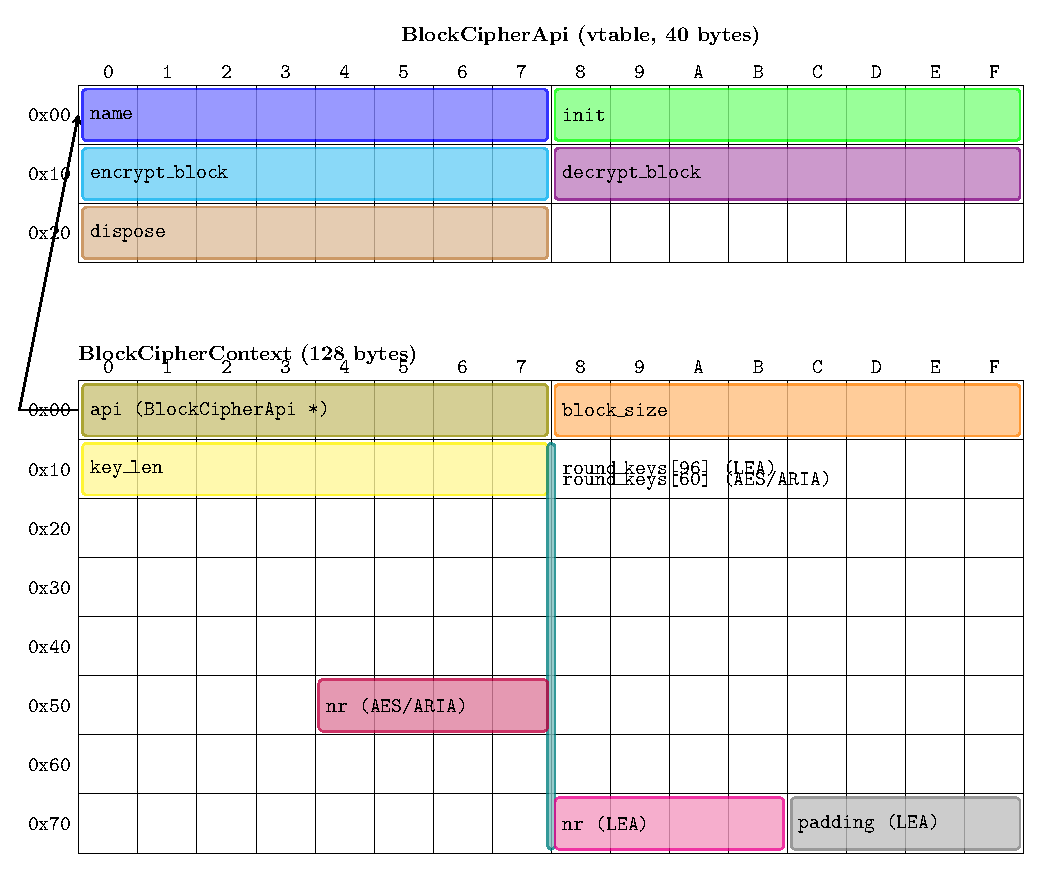
\includegraphics[scale=1]{memory_layout/BlockCipherApi.pdf}
%\end{figure}

\newpage
\begin{lstlisting}[style=cstyle, caption={include/block\_cipher/api\_block\_cipher.h}, captionpos=t]
/* Forward declaration for the context. */
typedef struct __BlockCipherContext__ BlockCipherContext;

typedef struct __BlockCipherApi__ {
	const char *cipher_name; /* e.g. "AES" or "MyCipher" */
	
	block_cipher_status_t (*cipher_init)(
		BlockCipherContext* cipher_ctx, 
		const u8* key, 
		size_t key_len, 
		size_t block_len, 
		BlockCipherDirection dir);
	block_cipher_status_t (*cipher_process)(
		BlockCipherContext* cipher_ctx, 
		const u8* in, 
		u8* out, 
		BlockCipherDirection dir);
	void (*cipher_dispose)(BlockCipherContext* cipher_ctx);
} BlockCipherApi;

typedef union __CipherInternal__ {
	struct __aes_internal__ {
		size_t block_size;      /* Typically must be 16 for AES */
		size_t key_len;         /* 16, 24, or 32 for AES-128/192/256 */
		/* max 60 for AES-256 */
		u32 round_keys[4 * (AES256_NUM_ROUNDS + 1)];     
		int nr;                 /* e.g., 10 for AES-128, 12, or 14... */
	} aes_internal;
	struct __aria_internal__ {
		size_t block_size;      /* Typically must be 16 for ARIA */
		size_t key_len;         /* 16, 24, or 32 for ARIA-128/192/256 */
		/* max 68 for ARIA-256 */
		u32 round_keys[4 * (ARIA256_NUM_ROUNDS + 1)];     
		int nr;                 /* e.g., 12 for ARIA-128, 14, or 16... */
	} aria_internal;
	struct __lea_internal__ {
		size_t block_size;      /* Typically must be 16 for LEA */
		size_t key_len;         /* 16, 24, or 32 for LEA-128/192/256 */
		/* max 192 for LEA-256 */
		u32 round_keys[6 * LEA256_NUM_ROUNDS];    
		int nr;                 /* e.g., 24 for LEA-128, 28, or 32... */
	} lea_internal;
} CipherInternal;

struct __BlockCipherContext__ {
	const BlockCipherApi *cipher_api;  
	CipherInternal cipher_state; /* Generic internal state for any cipher */
};
\end{lstlisting}

\begin{table}[h!]\centering
	\begin{tabular*}{\linewidth}{@{\extracolsep{\fill}}l|p{11cm}||l}
		\toprule
		Subsection & Description & Status \\
		\midrule
		2.1.1     & AES (Advanced Encryption Standard) & Drafted      \\
		2.1.2     & ARIA (Academy, Research Institute, and Agency)  & Drafted \\
		2.1.3     & LEA (Lightweight Encryption Algorithm) & Drafted \\
		\bottomrule
	\end{tabular*}
\end{table}
\newpage
\subsection{AES (Advanced Encryption Standard)}
\begin{table}[h!]
	\centering
	\renewcommand{\arraystretch}{1.25} % Increase row height
	\caption{Parameters of the Block Cipher AES (1-word = 32-bit)}
	\begin{tabular*}{\textwidth}{@{\extracolsep{\fill}}c c c c c c c}
		\toprule[1.2pt]
		\textbf{Alg.} & $\boldsymbol{n}$ (bit) & $\boldsymbol{k}$ (bit) & \textbf{\# of Rounds} & \textbf{RK Size} (bit) & \textbf{\# of RKs} & \textbf{Total RK Size} (bit) \\
		\midrule
		\textsf{AES--128} & 128 & 128 & 10 & 128 (4-word) & 11 & 1408 (44-word) \\
		\textsf{AES--192} & 128 & 192 & 12 & 128 (4-word) & 13 & 1664 (52-word) \\
		\textsf{AES--256} & 128 & 256 & 14 & 128 (4-word) & 15 & 1920 (60-word) \\
		\bottomrule[1.2pt]
	\end{tabular*}
\end{table}

%\begin{table}[h!]\centering\renewcommand{\arraystretch}{1.25} % Increase row height by 1.5 times
%	\caption{Parameters of the Block Cipher AES (1-word = 32-bit)}
%	\begin{tabular*}{\textwidth}{@{\extracolsep{\fill}}c||cccccc}
%		\toprule[1.2pt]
%		\multirow{3}{*}{Algorithms} & Block & Key & Number of & Round-Key & Number of & Total Size of\\
%		& Size & Length & Rounds &  Length & Round-Keys & Round-Keys \\
%		& ($N_b$-word) & ($N_k$-word) & ($N_r$)& (word) & ($N_r+1$)& ($N_b(N_r+1)$)\\
%		\hline\hline
%		\textsf{AES-128} & 4 & 4 & 10 & 4 & 11 & 44 (176-byte) \\
%		\textsf{AES-192} & 4 & 6 & 12 & 4 & 13 & 52 (208-byte) \\
%		\textsf{AES-256} & 4 & 8 & 14 & 4 & 15 & 60 (240-byte) \\
%		\bottomrule[1.2pt]
%	\end{tabular*}
%\end{table}

%\begin{tikzpicture}[>=stealth, node distance=0cm, scale=.9]
%	% Set font for nodes to a small monospace for clarity
%	\tikzstyle{every node}=[font=\footnotesize\ttfamily]
%	
%	% Dimensions and coordinates (assuming 64-bit, pointer = 8 bytes)
%	\def\ptrSize{0.5}    % height for an 8-byte field (in cm)
%	\def\ctxWidth{5.0}   % width of the BlockCipherContext struct box (in cm)
%	\def\apiWidth{4.0}   % width of the BlockCipherApi struct box (in cm)
%	
%	% BlockCipherContext structure box
%	\coordinate (ctxOrigin) at (0,0);                            % top-left corner of BlockCipherContext
%	\draw[draw, thick] (ctxOrigin) rectangle ++(\ctxWidth,-\ptrSize)
%	node[midway] {BlockCipherApi *api};                   % api pointer field
%	\draw[draw, thick] (0,-\ptrSize) rectangle ++(\ctxWidth,-5.0) 
%	node[midway] {uint8\_t internal\_data[256]};             % internal_data array field (256 bytes)
%	\draw[thick] (ctxOrigin) -- ++(0, -5.5);                     % left boundary line for context (extend to full height)
%	\draw[thick] (\ctxWidth, 0) -- ++(0, -5.5);                  % right boundary line for context
%	
%	% Offset markers for BlockCipherContext
%	\draw[thick] ($(ctxOrigin) + (0,0)$) -- ++(-3mm,0) node[left] {0x00};
%	\draw[thick] ($(ctxOrigin) + (0,-\ptrSize)$) -- ++(-3mm,0) node[left] {0x08};
%	\draw[thick] ($(ctxOrigin) + (0,-5.5)$) -- ++(-3mm,0) node[left] {0x108};
%	\draw[decorate, decoration={brace, amplitude=4pt}, thick]
%	(\ctxWidth + 0.1, -\ptrSize) -- node[right=4pt]{256 bytes} (\ctxWidth + 0.1, -5.5);
%	
%	% Label the struct
%	\node[above=2mm of ctxOrigin, anchor=west, font=\normalsize\bfseries] {BlockCipherContext (in memory)};
%	
%	% BlockCipherApi structure box (positioned to the right of context)
%	\coordinate (apiOrigin) at (\ctxWidth + 3.0, 0);            % top-left corner of BlockCipherApi (some gap to the right)
%	% Draw each field of BlockCipherApi as a rectangle
%	\draw[draw, thick] (apiOrigin) rectangle ++(\apiWidth,-\ptrSize)  
%	node[midway] {const char *name};
%	\draw[draw, thick] ($(apiOrigin)+(0,-\ptrSize)$) rectangle ++(\apiWidth,-\ptrSize)  
%	node[midway] {init};
%	\draw[draw, thick] ($(apiOrigin)+(0,-2*\ptrSize)$) rectangle ++(\apiWidth,-\ptrSize)  
%	node[midway] {encrypt\_block};
%	\draw[draw, thick] ($(apiOrigin)+(0,-3*\ptrSize)$) rectangle ++(\apiWidth,-\ptrSize)  
%	node[midway] {decrypt\_block};
%	\draw[draw, thick] ($(apiOrigin)+(0,-4*\ptrSize)$) rectangle ++(\apiWidth,-\ptrSize)  
%	node[midway] {dispose};
%	\draw[thick] (apiOrigin) -- ++(0, -5*\ptrSize);              % left boundary line for API struct
%	\draw[thick] ($(apiOrigin)+(\apiWidth,0)$) -- ++(0, -5*\ptrSize); % right boundary line for API struct
%	
%	% Offset markers for BlockCipherApi
%	\draw[thick] ($(apiOrigin) + (0,0)$) -- ++(-3mm,0) node[left] {0x00};
%	\draw[thick] ($(apiOrigin) + (0,-\ptrSize)$) -- ++(-3mm,0) node[left] {0x08};
%	\draw[thick] ($(apiOrigin) + (0,-2*\ptrSize)$) -- ++(-3mm,0) node[left] {0x10};
%	\draw[thick] ($(apiOrigin) + (0,-3*\ptrSize)$) -- ++(-3mm,0) node[left] {0x18};
%	\draw[thick] ($(apiOrigin) + (0,-4*\ptrSize)$) -- ++(-3mm,0) node[left] {0x20};
%	\draw[thick] ($(apiOrigin) + (0,-5*\ptrSize)$) -- ++(-3mm,0) node[left] {0x28};
%	
%	% Label the struct
%	\node[above=2mm of apiOrigin, anchor=west, font=\normalsize\bfseries] {BlockCipherApi (in memory)};
%	
%	% Pointer arrow from BlockCipherContext.api to BlockCipherApi struct
%	\coordinate (ctxApiPtr) at ($(ctxOrigin) + (\ctxWidth/2, -\ptrSize/2)$);   % center of ctx.api field
%	\coordinate (apiNameLeft) at ($(apiOrigin) + (0, -\ptrSize/2)$);           % left edge midpoint of API.name field
%	\draw[->, thick] (ctxApiPtr) -- (apiNameLeft);
%	
%	% Pointer arrow from BlockCipherApi.name to an example name string
%	\coordinate (apiNameRight) at ($(apiOrigin) + (\apiWidth, -\ptrSize/2)$);
%	\draw[->, thick] (apiNameRight) -- ++(1.5, 0) node[right] {“AES-128”};
%	
%	% Pointer arrows from function pointers to function code (illustrative)
%	\foreach \i/\name in {1/init(), 2/encrypt\_block(), 3/decrypt\_block(), 4/dispose()} {%
%		\coordinate (fieldRight\i) at ($(apiOrigin) + (\apiWidth, -\i*\ptrSize + \ptrSize/2)$);
%		\draw[->, thick] (fieldRight\i) -- ++(1.2, 0) node[right] {\name \,function};
%	}
%	
%	% Legend / notes
%	\node[anchor=west] at ($(ctxOrigin) + (0,-6.2)$) 
%	{\textit{Note: Arrows show pointer targets. “init() function” etc. indicate the actual code for those function pointers.}};
%\end{tikzpicture}
%
%% TikZ diagram of BlockCipherContext and BlockCipherApi (vtable) memory layout
%% (Assuming 64-bit system: pointers are 8 bytes, hence offsets increment by 0x08)
%\begin{tikzpicture}[font=\footnotesize\ttfamily, >=Stealth, scale=.8]
%	% Define dimensions
%	\def\ptrH{0.3}      % height for one pointer field (represents 8 bytes)
%	\def\halfPtrH{0.15} % half of pointer field height
%	\def\intH{9.6}      % height for 256-byte internal_data field (32 * \ptrH)
%	\def\halfIntH{4.8}  % half of internal_data field height
%	\def\ctxWidth{5}    % width of structure boxes
%	\def\vtWidth{5}
%	\def\funcWidth{5.5} % width of function implementation boxes
%	% X-coordinates for structures
%	\def\ctxX{0}        % BlockCipherContext X position
%	\def\vtX{6.5}       % BlockCipherApi (vtable) X position
%	\def\funcX{13}      % Function implementations X position
%	
%	% BlockCipherContext structure outline
%	\draw (\ctxX, 0) rectangle ({\ctxX + \ctxWidth}, {-(\ptrH + \intH)});
%	\draw (\ctxX, -\ptrH) -- ({\ctxX + \ctxWidth}, -\ptrH);  % divider between fields
%	% BlockCipherContext field labels
%	\node[anchor=west, inner sep=1mm] at (\ctxX, -\halfPtrH) {BlockCipherApi *api};
%	\node[anchor=west, inner sep=1mm] at (\ctxX, {-(\ptrH + \halfIntH)}) {u8 internal\_data[256]};
%	% BlockCipherContext offset labels (left side)
%	\node[anchor=east, fill=white, inner sep=1pt] at (\ctxX, 0) {0x00};
%	\node[anchor=east, fill=white, inner sep=1pt] at (\ctxX, -\ptrH) {0x08};
%	\node[anchor=east, fill=white, inner sep=1pt] at (\ctxX, {-(\ptrH + \intH)}) {0x108};
%	% BlockCipherContext size annotations (right side)
%	\node[anchor=west] at ({\ctxX + \ctxWidth + 1mm}, {-\halfPtrH - 0.05}) {8 bytes};
%	\node[anchor=west] at ({\ctxX + \ctxWidth + 1mm}, {-(\ptrH + \halfIntH)}) {256 bytes};
%	
%	% BlockCipherApi (vtable) structure outline
%	\draw (\vtX, 0) rectangle ({\vtX + \vtWidth}, {-5 * \ptrH});
%	\foreach \i in {1,...,4} { % horizontal lines for each vtable field
%		\draw (\vtX, {-\i * \ptrH}) -- ({\vtX + \vtWidth}, {-\i * \ptrH});
%	}
%	% BlockCipherApi vtable field labels
%	\node[anchor=west, inner sep=1mm] at (\vtX, -\halfPtrH) {const char *name};
%	\node[anchor=west, inner sep=1mm] at (\vtX, {-(1 * \ptrH + \halfPtrH)}) {init (function ptr)};
%	\node[anchor=west, inner sep=1mm] at (\vtX, {-(2 * \ptrH + \halfPtrH)}) {encrypt\_block (function ptr)};
%	\node[anchor=west, inner sep=1mm] at (\vtX, {-(3 * \ptrH + \halfPtrH)}) {decrypt\_block (function ptr)};
%	\node[anchor=west, inner sep=1mm] at (\vtX, {-(4 * \ptrH + \halfPtrH)}) {dispose (function ptr)};
%	% BlockCipherApi vtable offset labels (left side)
%	\node[anchor=east, fill=white, inner sep=1pt] at (\vtX, 0) {0x00};
%	\node[anchor=east, fill=white, inner sep=1pt] at (\vtX, { -1 * \ptrH }) {0x08};
%	\node[anchor=east, fill=white, inner sep=1pt] at (\vtX, { -2 * \ptrH }) {0x10};
%	\node[anchor=east, fill=white, inner sep=1pt] at (\vtX, { -3 * \ptrH }) {0x18};
%	\node[anchor=east, fill=white, inner sep=1pt] at (\vtX, { -4 * \ptrH }) {0x20};
%	\node[anchor=east, fill=white, inner sep=1pt] at (\vtX, { -5 * \ptrH }) {0x28};
%	% Brace to label the vtable structure
%	\draw[decorate, decoration={brace, mirror, amplitude=5pt}] (\vtX, { -5 * \ptrH }) -- (\vtX, 0)
%	node[midway, left=6pt]{BlockCipherApi (vtable)};
%	
%	% AES function implementation blocks
%	\node[draw, minimum width=\funcWidth cm, anchor=west, align=left, inner sep=2mm] (funcInit) 
%	at (\funcX, {-(1 * \ptrH + \halfPtrH)}) {aes\_init function implementation};
%	\node[draw, minimum width=\funcWidth cm, anchor=west, align=left, inner sep=2mm] (funcEnc)  
%	at (\funcX, {-(2 * \ptrH + \halfPtrH)}) {aes\_encrypt function implementation};
%	\node[draw, minimum width=\funcWidth cm, anchor=west, align=left, inner sep=2mm] (funcDec)  
%	at (\funcX, {-(3 * \ptrH + \halfPtrH)}) {aes\_decrypt function implementation};
%	\node[draw, minimum width=\funcWidth cm, anchor=west, align=left, inner sep=2mm] (funcDisp) 
%	at (\funcX, {-(4 * \ptrH + \halfPtrH)}) {aes\_dispose function implementation};
%	
%	% Pointer arrows showing relationships
%	\draw[->] ({\ctxX + \ctxWidth}, {-\halfPtrH}) -- (\vtX, {-\halfPtrH});
%	\draw[->] ({\vtX + \vtWidth}, {-(1 * \ptrH + \halfPtrH)}) -- (funcInit.west);
%	\draw[->] ({\vtX + \vtWidth}, {-(2 * \ptrH + \halfPtrH)}) -- (funcEnc.west);
%	\draw[->] ({\vtX + \vtWidth}, {-(3 * \ptrH + \halfPtrH)}) -- (funcDec.west);
%	\draw[->] ({\vtX + \vtWidth}, {-(4 * \ptrH + \halfPtrH)}) -- (funcDisp.west);
%\end{tikzpicture}


\begin{lstlisting}[style=cstyle, caption={include/block\_cipher/block\_cipher\_aes.h}, captionpos=t]
/* Get the AES block cipher vtable. */
const BlockCipherApi* get_aes_api(void);

void aes_set_encrypt_key(const u8 *key, size_t bytes, u32 *rk);
void aes_set_decrypt_key(const u8 *key, size_t bytes, u32 *rk);
void aes_encrypt(const u8 *in, u8 *out, const u32 *rk, int r);
void aes_decrypt(const u8 *in, u8 *out, const u32 *rk, int r);
\end{lstlisting}
\begin{lstlisting}[style=cstyle, caption={src/block\_cipher/block\_cipher\_aes.c}, captionpos=t]
/* Forward declarations of static functions. */
static block_cipher_status_t aes_init(
	BlockCipherContext *ctx, 
	const u8 *key, 
	size_t key_len, 
	size_t block_len, 
	BlockCipherDirection dir);
static block_cipher_status_t aes_process(
	BlockCipherContext *ctx, 
	const u8 *in,
	u8 *out, 
	BlockCipherDirection dir);
static void aes_dispose(BlockCipherContext *ctx);

/* The AES block cipher API. */
static const BlockCipherApi AES_API = {
	.cipher_name          = "AES",
	.cipher_init          = aes_init,
	.cipher_process       = aes_process,
	.cipher_dispose       = aes_dispose
};

/* Get the AES block cipher API. */
const BlockCipherApi *get_aes_api(void) { return &AES_API; }
\end{lstlisting}
\newpage

%\begin{lstlisting}
%/* 
%* AES Round Transformation (Highly Optimized)
%* 
%* I utilized loop unrolling, pointer arithmetic, and 
%* specific compiler extensions to ensure minimal overhead.
%* This is a simplified excerpt focusing on 128-bit keys.
%*/
%
%#include <stdint.h>
%#include <stddef.h>
%
%/* Example S-box for AES; typically a static const table. */
%static const uint8_t sbox[256] = {
%	/* 256 values omitted for brevity ... */
%};
%
%/* 
%* Inline function for SubBytes step using the S-box 
%* Leveraging GCC's __restrict to hint pointer usage.
%*/
%static inline void sub_bytes(uint8_t *__restrict block) {
%	for (int i = 0; i < 16; ++i) {
%		block[i] = sbox[block[i]];
%	}
%}
%
%/*
%* Inlined function for ShiftRows step.
%* Shifts the rows of the 4x4 byte matrix left by
%* varying offsets (0,1,2,3).
%*/
%static inline void shift_rows(uint8_t *__restrict block) {
%	/* Row 1 shift: 4 bytes are rearranged as needed */
%	uint8_t temp = block[1];
%	block[1]     = block[5];
%	block[5]     = block[9];
%	block[9]     = block[13];
%	block[13]    = temp;
%	
%	/* Row 2 shift: 4 bytes swap in pairs */
%	uint8_t temp1 = block[2];
%	uint8_t temp2 = block[6];
%	block[2]      = block[10];
%	block[6]      = block[14];
%	block[10]     = temp1;
%	block[14]     = temp2;
%	
%	/* Row 3 shift: 4 bytes are rearranged again */
%	temp          = block[3];
%	block[3]      = block[15];
%	block[15]     = block[11];
%	block[11]     = block[7];
%	block[7]      = temp;
%}
%
%/* 
%* Multiply operation in GF(2^8) for MixColumns 
%* using a small lookup to accelerate. 
%*/
%static inline uint8_t gm_mul(uint8_t a, uint8_t b) {
%	uint8_t r = 0;
%	for (int i = 0; i < 8; i++) {
%		if (b & 1) r ^= a;
%		uint8_t hi = (uint8_t)(a & 0x80);
%		a <<= 1;
%		if (hi) a ^= 0x1b; 
%		b >>= 1;
%	}
%	return r;
%}
%
%/*
%* MixColumns uses the gf_mul helper for each column in the block.
%* Four 4-byte columns are processed. This routine is unrolled 
%* for maximum performance with minimal overhead.
%*/
%static inline void mix_columns(uint8_t *__restrict block) {
%	for (int col = 0; col < 4; col++) {
%		uint8_t *c = block + (col << 2);
%		uint8_t a0 = c[0], a1 = c[1], a2 = c[2], a3 = c[3];
%		uint8_t r0 = gm_mul(a0, 2) ^ gm_mul(a1, 3) ^ a2 ^ a3;
%		uint8_t r1 = a0 ^ gm_mul(a1, 2) ^ gm_mul(a2, 3) ^ a3;
%		uint8_t r2 = a0 ^ a1 ^ gm_mul(a2, 2) ^ gm_mul(a3, 3);
%		uint8_t r3 = gm_mul(a0, 3) ^ a1 ^ a2 ^ gm_mul(a3, 2);
%		c[0] = r0; c[1] = r1; c[2] = r2; c[3] = r3;
%	}
%}
%
%/*
%* add_round_key merges the round subkey using XOR 
%* for the final step of each round.
%*/
%static inline void add_round_key(uint8_t *block, const uint8_t *round_key) {
%	for (int i = 0; i < 16; ++i) {
%		block[i] ^= round_key[i];
%	}
%}
%
%/*
%* This function performs one AES round:
%* SubBytes -> ShiftRows -> MixColumns -> AddRoundKey
%*/
%void aes_round_optimized(uint8_t *block, const uint8_t *round_key) {
%	sub_bytes(block);
%	shift_rows(block);
%	mix_columns(block);
%	add_round_key(block, round_key);
%}
%\end{lstlisting}

%\paragraph{Discussion of Optimization Techniques}
%
%\begin{itemize}
%	\item \textbf{Loop Unrolling:} By explicitly unrolling small loops (e.g., in \texttt{mix\_columns}), I minimized overhead and allowed the compiler to optimize register usage.
%	\item \textbf{Inline Functions:} Using \texttt{static inline} for repeated sub-steps avoids function-call overhead and permits further inlining by the compiler.
%	\item \textbf{\_\_restrict Keyword:} This GNU C extension hints that pointers do not overlap, helping the compiler optimize more aggressively.
%	\item \textbf{Pointer Arithmetic:} Rather than indexing in 2D, I calculated offsets with \texttt{block + (col << 2)} to reduce overhead and help the compiler precompute certain expressions.
%	\item \textbf{Bitwise Operations:} The gf\_mul routine is carefully written to exploit bit shifts and XOR in a constant-time style, though actual side-channel resistance may need further architecture-specific measures.
%\end{itemize}
%
%Although this code snippet is simplified to illustrate the core round transformation, the real library includes full key scheduling, final rounds (without \texttt{mix\_columns}), and thorough security reviews to avoid side-channel leaks.
%
%\paragraph{Security Considerations}
%
%Since cryptographic code can be sensitive to timing and side-channel attacks, I took these protective measures:
%
%\begin{itemize}
%	\item \textbf{Constant-Time Operations:} The S-box lookups and \texttt{gm\_mul} attempts to avoid data-dependent branching, though further hardware-specific adjustments may be necessary.
%	\item \textbf{Memory Clearing:} I zeroize key data in memory immediately when it is no longer needed, using a dedicated function that the compiler does not optimize away.
%	\item \textbf{Limited Exposure:} The internal routines are compiled as static where possible, preventing accidental usage from outside code.
%\end{itemize}
%
%\paragraph{Test Vectors}
%
%I used known NIST AES test vectors to verify correctness. The makefile includes a \texttt{make test} target that runs a C-based unit test suite, verifying:
%
%\begin{itemize}
%	\item \textbf{AES Single-Block Encryption:} Matches official known-answer tests.
%	\item \textbf{Randomized Stress Tests:} Random keys and plaintexts are encrypted and decrypted to ensure \texttt{plaintext == decryptedCiphertext}.
%\end{itemize}
%
%\paragraph{Performance Testing}
%I relied on microbenchmarking to confirm that the unrolled loops and inline expansions yielded measurable performance gains. For large data sets, using hardware instructions (e.g., AES-NI on x86) could further boost throughput, so the code checks CPU features at runtime if built with hardware-acceleration support.
%
%\paragraph{How I Maintained and Deployed the Module}
%
%From the earliest design stages, I versioned the module in a private Git repository. Whenever I introduced a new optimization or cryptographic transform, I documented it in the commit log, explaining my rationale and the performance or security impact.
%
%Once I gained confidence in the stability of the code, I created release tags (e.g., \texttt{v1.0}, \texttt{v1.1}), each accompanied by a changelog. For deployment within other projects, I have a \texttt{.pc} pkg-config file that allows easy \texttt{pkg-config --cflags --libs crypto\_module} usage, especially on Linux-based environments.
%
%\paragraph{Conclusions and Future Work}
%
%In this manual, I walked through my cryptographic C module from inception to deployment, describing in the first person how I wrote extremely optimized routines and upheld security best practices. Looking forward, I plan to:
%
%\begin{itemize}
%	\item Add alternative ciphers (e.g., ChaCha20) for platforms lacking AES hardware acceleration.
%	\item Improve side-channel countermeasures for hardware traces.
%	\item Integrate a robust test harness with fuzzing to detect memory safety bugs.
%\end{itemize}
%
%I hope that by sharing my insights on performance tuning, memory-safe design, and cryptographic caution, you find this module useful and educational.
%
%%\appendix
%\paragraph{Appendix: Example Build Script}
%
%Below is a small snippet of a \texttt{Makefile} portion I use to build and test the library:
%
%\begin{lstlisting}[language=make]
%CC      := gcc
%CFLAGS  := -O3 -Wall -Wextra -std=c11
%
%LIBNAME := libcrypto_module.a
%
%OBJS := aes_core.o test_vectors.o
%
%all: $(LIBNAME)
%
%$(LIBNAME): $(OBJS)
%@ar rcs $@ $^
%
%test: all
%@$(CC) $(CFLAGS) -o test_crypto test_main.c $(LIBNAME)
%@./test_crypto
%
%clean:
%rm -f $(OBJS) $(LIBNAME) test_crypto
%\end{lstlisting}
%
%\textbf{Usage}:
%\begin{verbatim}
%$ make
%$ make test
%\end{verbatim}
%
%\paragraph{References}
%
%\begin{itemize}
%	\item \textbf{NIST AES Standard:} \href{https://nvlpubs.nist.gov/nistpubs/FIPS/NIST.FIPS.197.pdf}{FIPS-197 (AES)}
%	\item \textbf{Intel AES-NI Reference:} \href{https://www.intel.com/content/www/us/en/developer/articles/technical/intel-advanced-encryption-standard-aes-instructions-set.html}{Intel AES-NI Docs}
%	\item \textbf{GNU Compiler Docs:} \href{https://gcc.gnu.org/onlinedocs/}{\texttt{gcc} Online Documentation}
%\end{itemize}

\subsection{ARIA (Academy, Research Institute, and Agency)}
\begin{table}[h!]
	\centering
	\renewcommand{\arraystretch}{1.25} % Increase row height
	\caption{Parameters of the Block Cipher ARIA (1-word = 32-bit)}
	\begin{tabular*}{\textwidth}{@{\extracolsep{\fill}}c c c c c c c}
		\toprule[1.2pt]
		\textbf{Alg.} & $\boldsymbol{n}$ (bit) & $\boldsymbol{k}$ (bit) & \textbf{\# of Rounds} & \textbf{RK Size} (bit) & \textbf{\# of RKs} & \textbf{Total RK Size} (bit) \\
		\midrule
		\textsf{ARIA--128} & 128 & 128 & 12 & 128 (4-word) & 13 & 1664 (52-word) \\
		\textsf{ARIA--192} & 128 & 192 & 14 & 128 (4-word) & 15 & 1920 (60-word) \\
		\textsf{ARIA--256} & 128 & 256 & 16 & 128 (4-word) & 17 & 2176 (68-word) \\
		\bottomrule[1.2pt]
	\end{tabular*}
\end{table}
\begin{lstlisting}[style=cstyle, caption={include/block\_cipher/block\_cipher\_aria.h}, captionpos=t]
/* Get the ARIA block cipher vtable. */
const BlockCipherApi* get_aria_api(void);

void aria_set_encrypt_key(const u8 *key, size_t bytes, u32 *rk);
void aria_set_decrypt_key(const u8 *key, size_t bytes, u32 *rk);
void aria_encrypt(const u8 *in, u8 *out, const u32 *rk, int r);
void aria_decrypt(const u8 *in, u8 *out, const u32 *rk, int r);
\end{lstlisting}
\begin{lstlisting}[style=cstyle, caption={src/block\_cipher/block\_cipher\_aria.c}, captionpos=t]
/* Forward declarations of static functions. */
static block_cipher_status_t aria_init(
	BlockCipherContext *ctx, 
	const u8 *key, 
	size_t key_len, 
	size_t block_len, 
BlockCipherDirection dir);
static block_cipher_status_t aria_process(
	BlockCipherContext *ctx, 
	const u8 *in, 
	u8 *out, 
	BlockCipherDirection dir);
static void aria_dispose(BlockCipherContext *ctx);

/* The ARIA block cipher API. */
static const BlockCipherApi ARIA_API = {
	.cipher_name    = "ARIA",
	.cipher_init    = aria_init,
	.cipher_process = aria_process,
	.cipher_dispose = aria_dispose
};
/* Get the ARIA block cipher API. */
const BlockCipherApi* get_aria_api(void) { return &ARIA_API; }
\end{lstlisting}

\newpage
\subsection{LEA (Lightweight Encryption Algorithm)}
\begin{table}[h!]
	\centering
	\renewcommand{\arraystretch}{1.25} % Increase row height
	\caption{Parameters of the Block Cipher LEA (1-word = 32-bit)}
	\begin{tabular*}{\textwidth}{@{\extracolsep{\fill}}c c c c c c c}
		\toprule[1.2pt]
		\textbf{Alg.} & $\boldsymbol{n}$ (bit) & $\boldsymbol{k}$ (bit) & \textbf{\# of Rounds} & \textbf{RK Size} (bit) & \textbf{\# of RKs} & \textbf{Total RK Size} (bit) \\
		\midrule
		\textsf{LEA--128}  & 128 & 128 & 24 & 192 (6-word) & 24 & 4608 (144-word) \\
		\textsf{LEA--192}  & 128 & 192 & 28 & 192 (6-word) & 28 & 5376 (168-word) \\
		\textsf{LEA--256}  & 128 & 256 & 32 & 192 (6-word) & 32 & 6144 (192-word) \\
		\bottomrule[1.2pt]
	\end{tabular*}
\end{table}
\begin{lstlisting}[style=cstyle, caption={include/block\_cipher/block\_cipher\_aria.h}, captionpos=t]
/* Get the LEA block cipher vtable. */
const BlockCipherApi* get_lea_api(void);

void lea_set_encrypt_key(const u8 *key, size_t bytes, u32 *rk);
void lea_set_decrypt_key(const u8 *key, size_t bytes, u32 *rk);
void lea_encrypt(const u8 *in, u8 *out, const u32 *rk, int r);
void lea_decrypt(const u8 *in, u8 *out, const u32 *rk, int r);
\end{lstlisting}
\begin{lstlisting}[style=cstyle, caption={src/block\_cipher/block\_cipher\_aria.c}, captionpos=t]
/* Forward declarations of static functions. */
static block_cipher_status_t lea_init(
	BlockCipherContext *ctx, 
	const u8 *key, 
	size_t key_len, 
	size_t block_len, 
	BlockCipherDirection dir);
static block_cipher_status_t lea_process(
	BlockCipherContext *ctx, 
	const u8 *in, 
	u8 *out, 
	BlockCipherDirection dir);
static void lea_dispose(BlockCipherContext *ctx);

/* The LEA block cipher API. */
static const BlockCipherApi LEA_API = {
	.cipher_name          = "LEA",
	.cipher_init          = lea_init,
	.cipher_process       = lea_process,
	.cipher_dispose       = lea_dispose
};
/* Get the LEA block cipher API. */
const BlockCipherApi *get_lea_api(void) { return &LEA_API; }
\end{lstlisting}
% Detailed content about supported block ciphers, usage examples, ASM optimizations

\newpage
%-----------------------------------------------------------------------
%  SECTION 2: MODES OF OPERATION
%-----------------------------------------------------------------------
\section{Modes of Operation}

\begin{lstlisting}[style=cstyle]
typedef struct __ModeOfOperationApi__ {
	const char *name;
	void (*init)( /* ... */ );
	void (*process)( /* ... */ );
	void (*dispose)( /* ... */ );
} ModeOfOperationApi;

typedef union __ModeInternal__ {
	struct __cbc_internal__ {
		/* ... */
	} cbc_internal;
	struct __ctr_internal__ {
		/* ... */
	} ctr_internal;
	struct __gcm_internal__ {
		/* ... */
	} gcm_internal;
	struct __ecb_internal__ {
		/* ... */
	} ecb_internal;
	
} ModeInternal;

typedef struct __ModeOfOperationContext__ {
	const ModeOfOperationApi *api;  // Pointer to the mode API
	BlockCipherContext cipher_ctx; // Block cipher context
	ModeInternal internal_data;     // Internal state for the mode
} ModeOfOperationContext;
\end{lstlisting}
%\begin{figure}[h!]
%	\begin{tikzpicture}[x=1cm, y=-0.07cm, font=\scriptsize, draw=black, >=Stealth, scale=.8]
	% BlockCipherContext outline
	\draw[thick] (0,0) rectangle ++(4,128);  % 128 bytes tall, 3 cm wide
	\draw[thick] (0,8) -- ++(4,0);          % line separating api vs internal_data at 8 bytes
	
	% BlockCipherContext labels and offsets
	\node[anchor=south, align=center, font=\small] at (2,0) {\textbf{ModeOfOperationContext}\\ \textbf{(800=8+792 bytes)}};
	\node[align=center] at (2,4) {\texttt{ModeOfOperationApi*}};
	\node[align=center] at (2,68) {\texttt{CipherInternal}\\ (union, 792 bytes)};
	
	\node[anchor=east] at (0,0) {{\tiny\ttfamily 0x000}};   % top address
	\node[anchor=east] at (0,8) {{\tiny\ttfamily 0x008}};
	\node[anchor=east] at (0,16) {{\tiny\ttfamily 0x010}};
	\node[anchor=east] at (0,24) {{\tiny\ttfamily 0x018}};
	\node[anchor=east] at (0,120) {{\tiny\ttfamily 0x318}};
	\node[anchor=east] at (0,128) {{\tiny\ttfamily 0x320}};
	
	% Expand union internal_data: AES, ARIA, LEA internal structures side-by-side
	% Base alignment line for union (offset 0x08 in context)
	\draw[densely dashed, color=gray!50] (4,8) -- ++(14,0) node[anchor=west]{\tiny\ttfamily 0x008};
	\draw[densely dashed, color=gray!50] (4,16) -- ++(14,0) node[anchor=west]{\tiny\ttfamily 0x010};
	\draw[densely dashed, color=gray!50] (4,24) -- ++(14,0) node[anchor=west]{\tiny\ttfamily 0x018};
	\draw[densely dashed, color=gray!50] (4,45) -- ++(14,0) node[anchor=west]{\tiny\ttfamily 0x108};
	\draw[densely dashed, color=gray!50] (4,53) -- ++(14,0) node[anchor=west]{\tiny\ttfamily 0x110};
	\draw[densely dashed, color=gray!50] (4,75) -- ++(14,0) node[anchor=west]{\tiny\ttfamily 0x128};
	\draw[densely dashed, color=gray!50] (4,83) -- ++(14,0) node[anchor=west]{\tiny\ttfamily 0x130};
	\draw[densely dashed, color=gray!50] (4,120) -- ++(14,0) node[anchor=west]{\tiny\ttfamily 0x318};
	\draw[densely dashed, color=gray!50] (4,128) -- ++(14,0) node[anchor=west]{\tiny\ttfamily 0x320};
	
	% AES internal struct (80 bytes used out of 120)
	\draw (5,8) rectangle ++(3,120);       % union size tall (for visual alignment)
	\draw (5,16) -- ++(3,0);
	\draw (5,24) -- ++(3,0);
	\draw (5,45) -- ++(3,0);
	\draw (5,53) -- ++(3,0);
	\node[anchor=south, align=center] at (6.5,8) {\textbf{aes\_internal}\\ \textbf{(8+8+240+8=264 bytes)}};
	\node at (6.5,12) {\texttt{size\_t block\_size}};
	\node at (6.5,20) {\texttt{size\_t key\_len}};
	\node[align=center] at (6.5,36) {\texttt{u32 round\_keys[60]} \\ (240 bytes)};
	\node at (6.5,49) {\texttt{int nr}\; (4 bytes)};
	\node[color=gray, align=center] at (6.5,90) {\footnotesize (unused\\ \footnotesize 528 bytes)};
	\filldraw[gray!70, opacity=.2] (5, 53) rectangle (8, 128);
	
	\filldraw[teal!70, opacity=.2] (5, 8) rectangle (8, 16);
	\filldraw[orange!70, opacity=.2] (5, 16) rectangle (8, 24);
	\filldraw[red!70, opacity=.2] (5, 24) rectangle (8, 45);
	\filldraw[blue!70, opacity=.2] (5, 45) rectangle (8, 53);
	
	% ARIA internal struct (same as AES, 80 bytes)
	\draw (9,8) rectangle ++(3,120);
	\draw (9,16) -- ++(3,0);
	\draw (9,24) -- ++(3,0);
	\draw (9,75) -- ++(3,0);
	\draw (9,83) -- ++(3,0);
	\node[anchor=south, align=center] at (10.5,8) {\textbf{aria\_internal}\\ \textbf{(8+8+272+8=296 bytes)}};
	\node at (10.5,12) {\texttt{size\_t block\_size}};
	\node at (10.5,20) {\texttt{size\_t key\_len}};
	\node[align=center] at (10.5,50) {\texttt{u32 round\_keys[68]} \\ (272 bytes)};
	\node at (10.5,79) {\texttt{int nr}\; (4 bytes)};
	\node[color=gray, align=center] at (10.5,104) {\footnotesize (unused\\ \footnotesize 496 bytes)};
	\filldraw[gray!70, opacity=.2] (9, 83) rectangle (12, 128);
	
	\filldraw[teal!70, opacity=.2] (9, 8) rectangle (12, 16);
	\filldraw[orange!70, opacity=.2] (9, 16) rectangle (12, 24);
	\filldraw[red!70, opacity=.2] (9, 24) rectangle (12, 75);
	\filldraw[blue!70, opacity=.2] (9, 75) rectangle (12, 83);
	
	% LEA internal struct (116 bytes + 4 bytes padding)
	\draw (13,8) rectangle ++(3,120);
	\draw (13,16) -- ++(3,0);
	\draw (13,24) -- ++(3,0);
	\draw (13,120) -- ++(3,0);
	\node[anchor=south, align=center] at (14.5,8) {\textbf{lea\_internal}\\ \textbf{(8+8+768+8=792 bytes)}};
	\node at (14.5,12) {\texttt{size\_t block\_size}};
	\node at (14.5,20) {\texttt{size\_t key\_len}};
	\node[align=center] at (14.5,64) {\texttt{u32 round\_keys[192]} \\ (768 bytes)};
	\node at (14.5,124) {\texttt{int nr}\; (4 bytes)};
	
	\filldraw[teal!70, opacity=.2] (13, 8) rectangle (16, 16);
	\filldraw[orange!70, opacity=.2] (13, 16) rectangle (16, 24);
	\filldraw[red!70, opacity=.2] (13, 24) rectangle (16, 120);
	\filldraw[blue!70, opacity=.2] (13, 120) rectangle (16, 128);
	
	% Brace to indicate union grouping
	\draw[decorate,decoration={brace,amplitude=4pt}] (16,130) -- node[below=4pt]{Union members (share same memory)} (5,130);
	
	% BlockCipherApi vtable structure (40 bytes)
	% Place vtable below (starting at y=140 for offset 0)
	\filldraw[blue!50, opacity=.8] (0, 160) rectangle (3, 168);
	\draw[thick] (0,160) rectangle ++(3,32);
	\draw[thick] (0,168) -- ++(3,0);
	\draw[thick] (0,176) -- ++(3,0);
	\draw[thick] (0,184) -- ++(3,0);
	%	\draw[thick] (0,192) -- ++(3,0);
	\node[anchor=south,align=center] at (1.5,160) {\textbf{BlockCipherApi (vtable)}\\ \textbf{8$\times$4=32 bytes}};
	\node at (1.5,164) {\texttt{const char* name}};
	\node at (1.5,172) {\texttt{void*}};
	\node at (1.5,180) {\texttt{void*}};
	%	\node at (1.5,188) {\texttt{void*}};
	\node at (1.5,188) {\texttt{void*}};
	
	% Arrows: BlockCipherContext.api -> vtable, and vtable function ptrs -> functions
	% API pointer arrow (from BCC.api field to vtable)
	\draw[->, thick] (0,4) -| (-1,4) -- (-1,164) -- ++(1,0);
	
	% Function implementation nodes for AES
	\node[draw, anchor=west, fill=magenta!10] (fn_init)        at (5,172) {\texttt{aes\_init(BlockCipherContext* ctx, /* ... */ );}};
	\node[draw, anchor=west, fill=green!10] (fn_encrypt)     at (5,180) {\texttt{aes\_process\_block(BlockCipherContext* ctx, /* ... */ );}};
	%	\node[draw, anchor=west, fill=lime!10] (fn_decrypt)     at (3.5,188) {\texttt{decrypt(BlockCipherContext* ctx, const u8* ct, u8* pt);}};
	\node[draw, anchor=west, fill=cyan!10] (fn_dispose)     at (5,188) {\texttt{dispose(BlockCipherContext* ctx);}};
	
	\draw[->] (3,172) -- (fn_init.west);
	\draw[->] (3,180) -- (fn_encrypt.west);
	%	\draw[->] (3,188) -- (fn_decrypt.west);
	\draw[->] (3,188) -- (fn_dispose.west);
\end{tikzpicture}
%\end{figure}

\subsection{Electronic Codebook (ECB)}
TBA
\subsection{Cipher Block Chaining (CBC)}
TBA
\subsection{Counter (CTR)}
TBA
\newpage
\section{Galois\;/\;Counter Mode (GCM)}
%\begin{center}
%	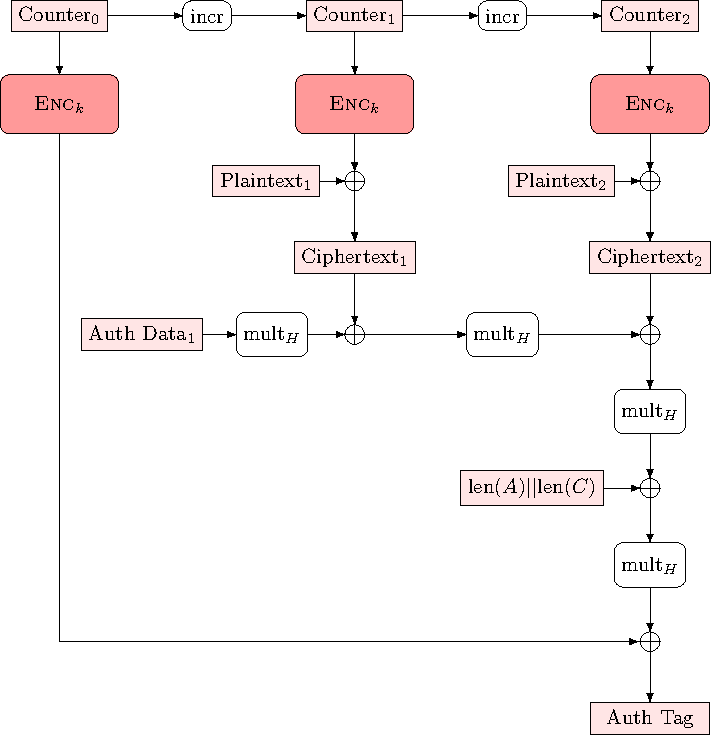
\includegraphics[scale=1]{tikz/GCM_encryption}
%\end{center}

\begin{figure}[h!]\centering
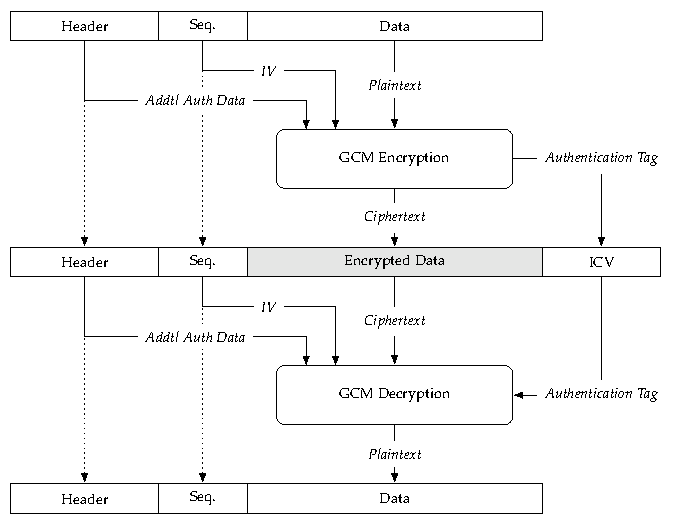
\includegraphics[scale=1.25]{tikz/gcm_mode}
\end{figure}

\subsection{Multiplication in $\GF(2^{128})$}
\begin{definition}
	Let \(\mathbb F_2 = \{0,1\}\) be the field with two elements.  Fix an irreducible polynomial
	\[
	f(x) \;=\; x^{128} + x^7 + x^2 + x + 1 
	\quad\in\; \mathbb F_2[x].
	\]
	Then
	\[
	\mathrm{GF}(2^{128}) \;=\; \mathbb F_2[x] \,\big/\,\bigl(f(x)\bigr)
	\]
	is the degree-\(128\) extension field.
\end{definition}
\begin{remark}
Every element \(\alpha\in\mathrm{GF}(2^{128})\) can be written uniquely as \[
\alpha \;=\; a_{127}x^{127} + a_{126}x^{126} + \cdots + a_1 x + a_0
\quad(a_i\in\{0,1\}).
\] We identify \(\alpha\) with the \(128\)-bit vector \((a_{0},\dots,a_{127})\in\F_2\).
\end{remark}

\paragraph{Polynomial Representation and Reduction}
Multiplication in \(\mathbb F_2[x]\) is carry-less:
\[
\left(\sum_i a_i x^i\right)\cdot\left(\sum_j b_j x^j\right)
=\sum_{i,j}\left(a_i b_j\right)\,x^{i+j}\,,
\]
with all additions mod 2.  To get the product in \(\mathrm{GF}(2^{128})\), we then reduce
the degree-\(\le 254\) result modulo \(f(x)\).

\paragraph{Bit-Level Algorithm}
We implement multiplication by a simple “shift-and-add” method with reduction on each
shift, often called \(\mathtt{xtime}\).

\begin{definition}[\,\(\mathtt{xtime}\) map\,]
	For \(v\in\mathrm{GF}(2^{128})\) represented as a 128-bit word, define
	\[
	\mathtt{xtime}(v) = 
	\begin{cases}
		v \ll 1, &\text{if the MSB of }v\text{ is }0,\\[6pt]
		(v \ll 1)\oplus R, &\text{if the MSB of }v\text{ is }1,
	\end{cases}
	\]
	where \(R\) is the bit-vector corresponding to the reduction polynomial
	\(x^7+x^2+x+1\).
\end{definition}

\paragraph{Pseudocode}
\ \\ \begin{algorithm}[H]
	\caption{Multiply two field elements \(a,b\in\mathrm{GF}(2^{128})\)}
	\label{alg:mul2}
	\begin{algorithmic}[1]
		\REQUIRE \(a,b\in\{0,1\}^{128}\) as 128-bit words  
		\ENSURE \(c = a\cdot b \bmod f(x)\)
		\STATE \(c \leftarrow 0\)  
		\STATE \(v \leftarrow a\)  
		\FOR{\(i=0\) to \(127\)}  
		\IF{bit \(i\) of \(b\) is 1}  
		\STATE \(c \leftarrow c \oplus v\)  
		\ENDIF  
		\STATE \(v \leftarrow \mathtt{xtime}(v)\)  
		\ENDFOR  
		\RETURN \(c\)
	\end{algorithmic}
\end{algorithm}



\paragraph{References:} 
\cite{NIST80038d},\;
\cite{McGrewViega2004gcm}

\newpage
%-----------------------------------------------------------------------
%  CHAPTER 4: RANDOM NUMBER GENERATOR (Placeholder)
%-----------------------------------------------------------------------
\section{Random Number Generator}
TBA
% Implementation details, entropy sources, usage examples

%-----------------------------------------------------------------------
%  CHAPTER 5: HASH FUNCTIONS (Placeholder)
%-----------------------------------------------------------------------
\section{Hash Functions}
\subsection{SHA-2 Algorithms}
TBA
\subsection{SHA-3 Algorithms}
TBA
\subsection{Lightweight Secure Hash (LSH)}
TBA
% Implementation details, supported hashes, ASM notes

%-----------------------------------------------------------------------
%  CHAPTER 6: MESSAGE AUTHENTICATION CODES (Placeholder)
%-----------------------------------------------------------------------
\section{Message Authentication Codes}
TBA
% Content about HMAC, CMAC, usage examples, best practices

%-----------------------------------------------------------------------
%  CHAPTER 7: KEY DERIVATION FUNCTIONS (Placeholder)
%-----------------------------------------------------------------------
\section{Key Derivation Functions}
TBA
% PBKDF, HKDF, usage in password hashing or key expansions

%-----------------------------------------------------------------------
%  CHAPTER 8: KEY EXCHANGE (Placeholder)
%-----------------------------------------------------------------------
\section{Diffie-Hellman Key Exchange}
TBA
% ECDH, DH, usage details, integration

%-----------------------------------------------------------------------
%  CHAPTER 9: SIGNATURE ALGORITHMS (Placeholder)
%-----------------------------------------------------------------------
\section{Signature Algorithms}
TBA
% ECDSA, RSA, usage patterns, performance tips

%%-----------------------------------------------------------------------
%%  CHAPTER 3: BUILD AND INTEGRATION (Placeholder)
%%-----------------------------------------------------------------------
\chapter{Build and Integration}

\section{Makefile Configuration and Overview}
This section describes the build system for the CryptoModule demo, driven by a single GNU Makefile. It covers compiler settings, directory layout, source discovery, and all available targets.

\subsection{Compiler, Flags, and Directories}
\begin{lstlisting}[numbers=none]
# Compiler and flags
CC      := gcc
CFLAGS  := -std=c99 -g -O2 -Wall -Wextra -I. -Iinclude -Isrc

# Executable name
TARGET  := cryptomodule-demo

# Output directories
OBJ_DIR := build
BIN_DIR := bin
\end{lstlisting}
\begin{itemize}
	\item \texttt{gcc} in C99 mode, with debug symbols (\texttt{-g}) and optimization (\texttt{-O2}).
	\item Warnings enabled (\texttt{-Wall -Wextra}), include paths set for project headers.
	\item Object files placed under \texttt{build/}, preserving the \texttt{src/} subdirectory structure; final binary in \texttt{bin/}.
\end{itemize}

\subsection{Automatic Source and Object Discovery}
\begin{lstlisting}[numbers=none]
# Find all .c files in src/ recursively
SRCS := $(shell find src -name '*.c')

# Map src/foo.c -> build/foo.o
OBJS := $(patsubst src/%.c,$(OBJ_DIR)/%.o,$(SRCS))
\end{lstlisting}

\newpage
\subsection{Usage Examples}
\begin{lstlisting}[numbers=none]
###############################################################################
# 1) build : compile + link
###############################################################################
build: $(BIN_DIR)/$(TARGET)

# Link step: gather all objects into a single executable
$(BIN_DIR)/$(TARGET): $(OBJS)
	@echo "[LINK] Linking objects to create $@"
	@mkdir -p $(BIN_DIR)
	$(CC) $(CFLAGS) $^ -o $@
# Compile step: For each .c -> .o
$(OBJ_DIR)/%.o: src/%.c
	@echo "[CC] Compiling $< into $@"
	@mkdir -p $(dir $@)
	$(CC) $(CFLAGS) -c $< -o $@
###############################################################################
# 2) run : run the resulting binary
###############################################################################
run: build
	@echo "[RUN] Running $(BIN_DIR)/$(TARGET)"
	@./$(BIN_DIR)/$(TARGET)

###############################################################################
# 3) clean : remove build artifacts
###############################################################################
clean:
@echo "[CLEAN] Removing build artifacts..."
	rm -rf $(OBJ_DIR) $(BIN_DIR)
	@echo "[CLEAN] Removing *.req and *.rsp files in testvectors folder..."
	find testvectors -type f \( -name '*.req' -o -name '*.rsp' \) -delete

###############################################################################
# 4) rebuild : clean + build
###############################################################################
rebuild: clean build

###############################################################################
# 5) valgrind : run the binary under Valgrind for memory checking
###############################################################################
valgrind: build
	@echo "[VALGRIND] Running Valgrind..."
	valgrind --leak-check=full ./$(BIN_DIR)/$(TARGET)
\end{lstlisting}

\begin{description}
	\item[\texttt{make build}] Compile (\texttt{.c → .o}) and link (\texttt{.o → executable}).
	\item[\texttt{make run}] Build if necessary, then execute \texttt{bin/cryptomodule-demo}.
	\item[\texttt{make clean}] Remove \texttt{build/}, \texttt{bin/}, and any \texttt{*.req}/\texttt{*.rsp} in \texttt{testvectors/}.
	\item[\texttt{make rebuild}] Alias for \texttt{clean} followed by \texttt{build}.
	\item[\texttt{make valgrind}] Build, then run under Valgrind for memory-leak checks.
\end{description}
% Makefile overview, linking instructions, library creation
%
%%-----------------------------------------------------------------------
%%  CHAPTER 4: TESTING (Placeholder)
%%-----------------------------------------------------------------------
%\chapter{Testing}
%% Unit tests, integration tests, reference vectors

%%-----------------------------------------------------------------------
%%  CHAPTER 5: FAQ / TROUBLESHOOTING (Placeholder)
%%-----------------------------------------------------------------------
%\chapter{FAQ / Troubleshooting}
%% Common errors, solutions, performance tuning

\newpage
\section{Example: Main Function for Block‐Cipher KATs}
\begin{lstlisting}[caption={Invoke known-answer tests for AES block ciphers},label={lst:main-kat},captionpos=t]
int main(void) {
	KAT_TEST_BLOCKCIPHER(BLOCK_CIPHER_AES128);
	KAT_TEST_BLOCKCIPHER(BLOCK_CIPHER_AES192);
	KAT_TEST_BLOCKCIPHER(BLOCK_CIPHER_AES256);
	return 0;
}
\end{lstlisting}
\begin{lstlisting}[]
@>$ make rebuild
@>$ make run
\end{lstlisting}

\begin{figure}[h!]\centering
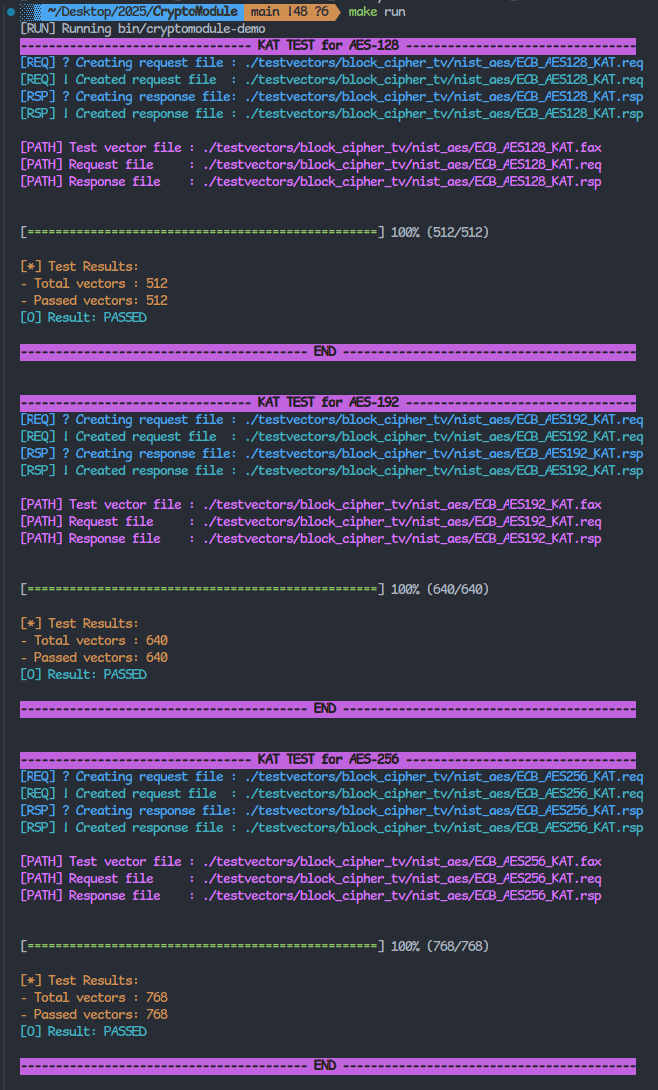
\includegraphics[scale=.65]{images/make_run}
\end{figure}

\newpage
\chapter{Analysis LIBECC}
\section{Words}

\subsection{Types}

\subsection*{Formalization of Fixed‐Width Integer Types}

% 1. The mathematical domains
\[
\mathbb{Z}_{2^k}
\;\coloneqq\;
\{\,n\in\mathbb{Z}\mid 0\le n < 2^k\},
\quad k\in\{8,16,32,64\}.
\]

% 2. Type‐to‐domain correspondence
\begin{align*}
	\mathrm{uint8\_t}  &\equiv \mathbb{Z}_{2^8},\\
	\mathrm{uint16\_t} &\equiv \mathbb{Z}_{2^{16}},\\
	\mathrm{uint64\_t} &\equiv \mathbb{Z}_{2^{64}}.
\end{align*}

% 3. Conditional definition of uint32_t
Let \(\mathit{WORDSIZE}\in\{16,32,64\}\) be the platform word size (in bits).  Then
\[
\mathrm{uint32\_t}
\;\equiv\;
\mathbb{Z}_{2^{32}}
\quad\text{with underlying C type}
\quad
\begin{cases}
	\texttt{unsigned long},&\text{if }\mathit{WORDSIZE}=16,\\
	\texttt{unsigned int},&\text{otherwise.}
\end{cases}
\]

% 4. Size‐type definitions
\[
\mathrm{size\_t}\;\equiv\;\mathbb{N}_0
\quad\text{(all nonnegative integers)},\qquad
\mathrm{ssize\_t}\;\equiv\;\mathbb{Z}.
\]

% 5. Macros for maximum values
\[
\mathrm{UINT}k\_\mathrm{MAX} \;=\; 2^k - 1,
\quad k\in\{8,16,32,64\}.
\]
In particular,
\[
\mathrm{UINT8\_MAX}=2^8-1,\;
\mathrm{UINT16\_MAX}=2^{16}-1,\;\dots
\]

% 6. Compile‐time sanity checks
The union
\[
\texttt{check\_data\_types}
\;:\equiv\;
\bigwedge_{k\in\{8,16,32,64\}}
%\bigl(\sizeof(\mathrm{uint}k\_t)=k\bigr)
\]
%encodes the requirement that each $\mathrm{uint}k\_t$ really occupies $k$ bits.

% 7. Constant‐literal macros
For any literal constant \(c\),
\[
\mathrm{UINT}k\_C(c)
\;:=\;
\bigl(\mathrm{uint}k\_t\bigr)\,c,
\quad k\in\{8,16,32,64\}.
\]

\section{Parameters}

\begin{lstlisting}[style=cstyle, caption={ec\_params\_external.h}, captionpos=t]
#ifndef __EC_PARAMS_EXTERNAL_H__
#define __EC_PARAMS_EXTERNAL_H__
#include <crypto/words/words.h>
typedef struct {
	const u8 *buf;
	const u8 buflen;
} ec_str_param;

typedef struct {
	/*
	* Prime p:
	*  o p_bitlen = bitsizeof(p)
	*/
	const ec_str_param *p;
	const ec_str_param *p_bitlen;
	
	/*
	* Precomputed Montgomery parameters:
	*  o r = 2^bitsizeof(p) mod p
	*  o r_square = 2^(2*bitsizeof(p)) mod p
	*  o mpinv = -p^-1 mod B
	* where B = 2^(bitsizeof(word_t))
	*/
	const ec_str_param *r;
	const ec_str_param *r_square;
	const ec_str_param *mpinv;
	
	/*
	* Precomputed division parameters:
	*  o p_shift = nn_clz(p)
	*  o p_normalized =  p << p_shift
	*  o p_reciprocal = floor(B^3/(DMSW(p_normalized) + 1)) - B
	* where B = 2^(bitsizeof(word_t))
	*/
	const ec_str_param *p_shift;
	const ec_str_param *p_normalized;
	const ec_str_param *p_reciprocal;
	
	/* Curve coefficients and number of points */
	const ec_str_param *a;
	const ec_str_param *b;
	const ec_str_param *curve_order;
	
	/*
	* Projective coordinates of generator
	* and order and cofactor of associated subgroup.
	*/
	const ec_str_param *gx;
	const ec_str_param *gy;
	const ec_str_param *gz;
	const ec_str_param *gen_order;
	const ec_str_param *gen_order_bitlen;
	const ec_str_param *cofactor;
	
	/* OID and pretty name */
	const ec_str_param *oid;
	const ec_str_param *name;
} ec_str_params;

#endif /* __EC_PARAMS_EXTERNAL_H__ */
\end{lstlisting}
\begin{lstlisting}[style=cstyle]
content...
\end{lstlisting}
\begin{lstlisting}[style=cstyle]
content...
\end{lstlisting}
\begin{lstlisting}[style=cstyle]
content...
\end{lstlisting}
\begin{lstlisting}[style=cstyle]
content...
\end{lstlisting}

\newpage
\chapter{Specification of ECDSA (secp256r1)}
\begin{table}[ht]\centering\ttfamily
\begin{tabular}{lp{12cm}}
{\normalfont\textbf{Parameter}} & {\normalfont\textbf{Value}} \\
$p$ & 0xffffffff00000001000000000000000000000000ffffffffffffffffffffffff \\
$a$ & 0xffffffff00000001000000000000000000000000fffffffffffffffffffffffc \\
$b$ & 0x5ac635d8aa3a93e7b3ebbd55769886bc651d06b0cc53b0f63bce3c3e27d2604b \\
$G$ & (0x6b17d1f2e12c4247f8bce6e563a440f277037d812deb33a0f4a13945d898c296, 0x4fe342e2fe1a7f9b8ee7eb4a7c0f9e162bce33576b315ececbb6406837bf51f5) \\
$n$ & 0xffffffff00000000ffffffffffffffffbce6faada7179e84f3b9cac2fc632551 \\
$h$ & 0x1
\end{tabular}
\end{table}

\begin{lstlisting}[style=cstyle]
	content...
\end{lstlisting}

\newpage
%\adjustbox{scale=2}{\[
%\underbrace{\textsf{NTT}}_{\text{Barrett}}\longrightarrow
%\underbrace{\textsf{Pointwise}}_{\text{Montgomery}}\longrightarrow
%\underbrace{\textsf{iNTT}}_{\text{Barrett}}
%\]}

\newpage

\bibliography{bibliography}

\newpage
\appendix
%-----------------------------------------------------------------------
%  CHAPTER 13: APPENDICES (Placeholder)
%-----------------------------------------------------------------------
\chapter*{Appendices}
TBA
% Glossary, references, external documentation
\fi

% CHAPTER 9
%\section*{References}
%\addcontentsline{toc}{chapter}{References} % This adds "References" to your Table of Contents

% The 'alpha' style creates labels like [BEF17] from the citation key.
\bibliographystyle{alpha}

\begin{thebibliography}{99}
	
	\bibitem[BEF17]{libecc-github}
	Ryad Benadjila, Arnaud Ebalard, and Jean-Pierre Flori.
	\newblock \emph{libecc: A lightweight and built-in ECC library}.
	\newblock GitHub repository, 2017.
	\newblock \url{https://github.com/libecc/libecc}, (Accessed: June 10, 2025).
	
	\bibitem[CMR+23]{nist-sp-800-186}
	Lily Chen, Dustin Moody, Andrew Regenscheid, et~al.
	\newblock \emph{{NIST Special Publication 800-186, Recommendations for Discrete
			Logarithm-based Cryptography: Elliptic Curve Domain Parameters}}.
	\newblock U.S. Department of Commerce, Gaithersburg, MD, February 2023.
	
	\bibitem[NIST13]{nist-fips-186-4}
	National Institute of Standards and Technology.
	\newblock \emph{{FIPS PUB 186-4, Digital Signature Standard (DSS)}}.
	\newblock U.S. Department of Commerce, Gaithersburg, MD, July 2013.
	
	\bibitem[NIST23]{nist-fips-186-5}
	National Institute of Standards and Technology.
	\newblock \emph{{FIPS PUB 186-5, Digital Signature Standard (DSS)}}.
	\newblock U.S. Department of Commerce, Gaithersburg, MD, February 2023.
	
	\bibitem[Por13]{rfc6979}
	Thomas Pornin.
	\newblock \emph{{RFC 6979: Deterministic Usage of the Digital Signature
			Algorithm (DSA) and Elliptic Curve Digital Signature Algorithm (ECDSA)}}.
	\newblock Internet Engineering Task Force, August 2013.
	
\end{thebibliography}

\appendix
\chapter{Integrated Makefile for Applications}
\begin{verbatim}
├── include
│   └── crypto
│       ├── ...
├── lib
│   ├── libarith.a
│   ├── libec.a
│   └── libsign.a
├── src
│   ├── filecheck_ecc.c
│   ├── generate_file.py
│   ├── generate_logs.py
│   ├── logaggregator_ecc.c
│   └── logtool_ecc.c
\end{verbatim}

\vfill
\section*{Build without Makefile}

\begin{lstlisting}[numbers=none]
mkdir -p obj bin
gcc -std=c99 -Wall -Wextra -O2 -Iinclude -c src/filecheck_ecc.c -o obj/filecheck_ecc.o
gcc -std=c99 -Wall -Wextra -O2 -Iinclude -o bin/filecheck_ecc obj/filecheck_ecc.o \
	lib/libarith.a \
	lib/libec.a \
	lib/libsign.a

gcc -std=c99 -Wall -Wextra -O2 -Iinclude -c src/logtool_ecc.c -o obj/logtool_ecc.o
gcc -std=c99 -Wall -Wextra -O2 -Iinclude -o bin/logtool_ecc \
	obj/logtool_ecc.o \
	lib/libarith.a \
	lib/libec.a \
	lib/libsign.a

gcc -std=c99 -Wall -Wextra -O2 -Iinclude -c src/logaggregator_ecc.c -o obj/logaggregator_ecc.o
gcc -std=c99 -Wall -Wextra -O2 -Iinclude -o bin/logaggregator_ecc \
	obj/logaggregator_ecc.o \
	lib/libarith.a \
	lib/libec.a \
	lib/libsign.a
\end{lstlisting}
\newpage
\section*{Build with Makefile}
\begin{lstlisting}[numbers=none]
CC      = gcc
CFLAGS  = -std=c99 -Wall -Wextra -O2 -Iinclude

SRCDIR  = src
OBJDIR  = obj
BINDIR  = bin
LIBDIR  = lib

# Your tools
TOOLS   = filecheck_ecc logtool_ecc logaggregator_ecc

# Object files
OBJS    = \
	$(OBJDIR)/common_utils.o \
	$(OBJDIR)/filecheck_ecc.o \
	$(OBJDIR)/logtool_ecc.o \
	$(OBJDIR)/logaggregator.o \

all: prep $(addprefix $(BINDIR)/, $(TOOLS))

prep:
	mkdir -p $(OBJDIR) $(BINDIR)

# Compile sources
$(OBJDIR)/%.o: $(SRCDIR)/%.c
	$(CC) $(CFLAGS) -c $< -o $@

# Link filecheck_ecc
$(BINDIR)/filecheck_ecc: $(OBJDIR)/filecheck_ecc.o
	$(CC) $(CFLAGS) -o $@ $^ \
		$(LIBDIR)/libarith.a $(LIBDIR)/libec.a $(LIBDIR)/libsign.a

# Link logtool_ecc
$(BINDIR)/logtool_ecc: $(OBJDIR)/logtool_ecc.o
	$(CC) $(CFLAGS) -o $@ \
		$^ \
		$(LIBDIR)/libarith.a \
		$(LIBDIR)/libec.a \
		$(LIBDIR)/libsign.a

# Link logaggregator (if it uses ECDSA too)
$(BINDIR)/logaggregator_ecc: $(OBJDIR)/logaggregator_ecc.o
	$(CC) $(CFLAGS) -o $@ \
		$^ \
		$(LIBDIR)/libarith.a \
		$(LIBDIR)/libec.a \
		$(LIBDIR)/libsign.a

clean:
rm -rf $(OBJDIR) $(BINDIR)

.PHONY: all prep clean

\end{lstlisting}

\end{document}
